\pagestyle{port}
\chapter{Argumentar e convencer}
\markboth{Módulo 1}{}

\colorsec{Habilidades do SAEB}

\begin{itemize}

  \item Identificar o uso de recursos persuasivos em textos verbais e não verbais.

  \item Identificar teses, opiniões, posicionamentos explícitos e argumentos em textos.

\end{itemize}

\colorsec{Habilidades da BNCC} 

\begin{itemize}

  \item EF67LP05, EF67LP07.

\end{itemize}

\conteudo{A todo momento estamos diante de textos, imagens e conteúdos que
pretendem transmitir mensagens. Alguns tipos de textos pretendem
convencer sobre a necessidade de um produto ou serviço, informar sobre
algum assunto ou situação e divulgar conhecimentos. Para que um texto
seja convincente, alguns aspectos devem ser observados: a linguagem
adequada ao público a que se destina a informação, o uso de recursos não
verbais e a forma como são veiculados tais textos. Tanto a recepção
quanto a produção de textos devem atentar-se a estes detalhes. Portanto,
é necessário que algumas características e recursos sejam reconhecidos
para que haja questionamento e, com isso, embasar a formação de nossas
opiniões, valores e ações. Em um mundo onde a informação chega de forma
cada vez mais imediata, por meio de redes sociais e aplicativos de
comunicação, deve-se estar atento a tais recursos e à forma com que
somos influenciados por eles. Por isso, é importante a compreensão de
que toda comunicação parte de uma intenção. Nas notícias, em campanhas
informativas ou publicitárias, nota-se a adoção de discursos e demais
recursos persuasivos. Discursos persuasivos são, portanto, elementos que
têm como objetivo convencer ou influenciar uma audiência a aceitar uma
ideia, um produto, uma posição política, um comportamento, propor uma
mudança de hábito ou conscientizar sobre determinado tema. O objetivo do
discurso persuasivo é fazer com que o ouvinte ou leitor adote uma
posição ou tome uma ação específica. Com atenção, pode-se aprender a
notar de que forma são elaborados os discursos persuasivos em campanhas
publicitárias, debates políticos, discursos de vendas, entre outros
contextos tais como notícias e reportagens.

%Paulo: este autor fez, ao final do conteúdo, extensas orientações ao professor. Coloquei-as todas em \coment{}

\coment{Professor(a), relembre os principais gêneros textuais que utilizam
recursos verbais e não verbais, questione sobre os gêneros que os alunos conhecem.
Estimule os estudantes a pensar sobre as funções dos argumentos
persuasivos, mostre como podem servir para a formação de opinião no caso
de textos jornalísticos, ou para convencimento nos casos de textos
publicitários. Relembre também a necessidade de critério e rigor técnico
no caso de textos de divulgação científica.

Utilize o exemplo para explicar as funções dos recursos verbais e não
verbais e estimule os estudantes na identificação das associações que
podem ser feitas entre as imagens e as palavras. Chame a atenção para a
citação dos órgãos oficiais e ressalte que esse tipo de referência pode
tornar um texto mais ou menos confiável por conta da possibilidade de
confrontar e questionar os dados apontados. Relembre os estudantes sobre
o uso de recursos persuasivos em demais gêneros textuais, apontando
também para suas especificidades quanto ao público alvo, função
comunicativa e meios de veiculação.}

\colorsec{Atividades}

\num{1} De acordo com seus conhecimentos, escreva dois tipos de recursos persuasivos 
presentes em campanhas publicitárias.

\linhas{2}
\cvoment{Linguagem objetiva, clara e direta; utilização de recursos verbais e não verbais;
escolha de fontes, cores e imagens que chamem a atenção do público alvo, entre outras.}

\num{2} Sobre os textos de divulgação científica assinale (V) para as afirmações verdadeiras e (F) para as afirmações falsas:

( ) Apresentam linguagem de difícil compreensão.

( ) Utilizam apenas recursos não verbais.

( ) Pretendem convencer.

( ) Apresentam linguagem objetiva.

\coment{F, F, V, V}

Textos de divulgação científica apresentam linguagem clara e objetiva
para divulgar conhecimentos científicos de forma acessível para o
público em geral e neles podem-se utilizar recursos não verbais tais como gráficos
e tabelas para apresentar os resultados descritos.

Leia a sentença a seguir e responda as questões. 

A dieta vegetariana é muito mais saudável. Cortar no consumo de animais reduz
o risco de colesterol alto, previne vários cancros, aumenta a energia e ajuda a
controlar o peso.

\num{3} Qual a afirmação principal do texto?

\linhas{1}
\coment{A afirmação principal é a de que a dieta vegetariana é mais saudável.}

\num{4} Quais argumentos baseiam a afirmação principal?

\linhas{2}
\coment{Os argumentos que baseiam a afirmação principal são: a dieta vegetariana
reduz o risco de colesterol alto, diminui as chances de desenvolver
vários tipos de câncer e ajuda no controle de peso.}

Leia a notícia abaixo e responda o que se pede:

\begin{quote}

\textbf{Estudo em sete estados aponta que uma mulher é vítima de
violência a cada quatro horas}

\emph{Rede de Observatórios da Segurança registrou 2.423 casos de
violência contra a mulher na Bahia, Ceará, Maranhão, Pernambuco, Piauí,
Rio de Janeiro e São Paulo em 2022. Foram 495 feminicídios.}

Um estudo com dados de sete estados brasileiros aponta que, em 2022, uma
mulher foi vítima de violência a cada quatro horas: foram 2.423 casos
--- e 495 deles terminaram em morte.

O estado de Pernambuco também passou a liderar os números de
transfeminicídios --- posição ocupada pelo Ceará nos últimos dois
anos. Segundo a pesquisadora da Rede em Pernambuco, Dália Celeste, essa
condição se dá pela negligência do governo. ``Houve um silenciamento e a
omissão do governo em relação à criação de políticas públicas mesmo após
a onda de ataques transfóbicos em 2021. Corpos trans e travestis passam
por um processo de desumanização e são vistos como corpos que não
deveriam existir, o que alimenta os crimes de ódio'' 

\end{quote}

\fonte{Priscilla Moraes. G1. Estudo em sete estados aponta que uma mulher é vítima de
violência a cada quatro horas. Disponível em: https://g1.globo.com/rj/rio-de-janeiro/noticia/2023/03/06/estudo-em-sete-estados-aponta-que-uma-mulher-e-vitima-de-violencia-a-cada-quatro-horas.ghtml}Acesso: 19 mai. 2023}

\num{5} O título da notícia pretende chamar a atenção para um assunto de utilidade pública. Que assunto é esse?

\linhas{2}
\coment{O título da notícia traz números alarmantes sobre a quantidade de casos
de violência contra a mulher em sete estados brasileiros.}

\num{6} Segundo as informações do corpo da notícia, relacione as colunas:

\begin{table}[]
\begin{tabular}{ll}
\begin{tabular}[c]{@{}l@{}}(I) Ceará\\ (II) Pernambuco\end{tabular} & \begin{tabular}[c]{@{}l@{}}(   ) O segundo colocado em número de casos de feminicídio.\\ (   ) Estado onde ocorre pelo menos um caso a cada dois dias.\\ (   ) O primeiro colocado em número de casos de transfeminícidio.\\ (   ) O primeiro colocado em número de casos de transfeminicídio nos anos anteriores.\end{tabular}
\end{tabular}
\end{table}

\coment{(II) O segundo colocado em número casos de feminicídio. 
(II) Estado onde ocorre pelo menos um caso a cada dois dias.
(II) O primeiro colocado em número de casos de transfeminícidio.
(I) O primeiro colocado em número de casos de transfeminicídio nos anos anteriores.}

\num{7} A notícia traz uma nova informação sobre violência contra mulher. Que informação é essa?

\linhas{2}
\coment{A notícia traz dados sobre transfeminicídio, que diz respeito aos homicídios de mulheres trans.}

\num{8} Segundo o texto da notícia, qual a principal motivação dos crimes de transfeminicídio no estado de Pernambuco?

\linhas{4}
\coment{Segundo a matéria, a omissão do governo em promover políticas públicas
contra os crimes de ódio é fator que influenciam no aumento dos
casos no estado de Pernambuco.}

\num{9} A matéria deixa claro que crimes de transfobia podem ser considerados um crime específico.
Que tipo de crime é esse? Copie do texto o trecho em que a autora faz essa afirmação.

\linhas{5}
\coment{Segundo a matéria, crimes de transfobia podem ser considerados crimes de ódio. O trecho 
em que a pesquisadora argumenta sobre a afirmação é: ``Corpos trans e travestis passam 
por um processo de desumanização e são vistos como corpos que não deveriam existir, o que
alimenta os crimes de ódio''.} 

\num{10} Na notícia apresentada, pode-se observar a citação direta da fala de
uma pesquisadora, representante de uma organização oficial que trabalha
com o tema do qual trata a matéria. O que este tipo de recurso confere
ao texto, no que diz respeito à confiabilidade das informações trazidas?

\linhas{3}
\coment{Ao trazer as fontes e citar nomes de pessoas envolvidas em grupos e
organizações oficiais, a matéria se torna mais confiável e os dados
podem ser questionados, pesquisados e confrontados pelo leitor.}

\colorsec{Treino}

\num{1}

\begin{quote}
Ghidinelli destacou que os países também devem trabalhar juntos e em
todos os setores, pois a malária não é apenas uma questão de saúde, mas
que também está ligada à economia, ao trabalho e ao meio ambiente. ``A
migração econômica de áreas endêmicas é um grande motor da malária em
nossa região e os mosquitos não conhecem fronteiras'', disse ele. ``A
eliminação só pode ser alcançada se as Américas consolidarem os esforços
para alcançar a meta de zero malária''.
\end{quote}

\fonte{Organização Pan-Americana da Saúde. Intervenções locais são cruciais para atingir o objetivo de eliminação da malária. Disponível em
https://www.paho.org/pt/noticias/4-11-2022-intervencoes-locais-sao-cruciais-para-atingir-objetivo-eliminacao-da-malaria.
Acesso em: 19 mai. 2023.}

De acordo com o texto a malária não é apenas uma questão de saúde, pois:

\begin{escolha}

  \item a migração das pessoas em áreas endêmicas ajuda a espalhar a doença.

  \item os países da América não tem nenhuma meta para eliminar a doença.

  \item os mosquitos não migram de uma localidade para a outra. 

  \item os mosquitos não conhecem fronteiras de natureza social e política.

\end{escolha}

\coment{SAEB: Identificar teses, opiniões, posicionamentos explícitos e
argumentos em textos.

BNCC: EF67LP05 -- Identificar e avaliar teses/opiniões/posicionamentos explícitos 
e argumentos em textos argumentativos (carta de leitor, comentário, artigo de opinião,
resenha crítica etc.), manifestando concordância ou discordância.

a)Correta. Segundo o texto, motivadas por questões econômicas, as pessoas migram de áreas 
assoladas pela doença para outras, espalhando a doença.
b)Incorreta. No texto, alude-se à meta dos governos de erradicar a doença.
c)Incorreta. No texto, afirma-se que o mosquito pode migrar de uma área para outra.
d)Incorreta. No texto, pode-se ler a afirmação de que o mosquito não conhece fronteiras 
e por isso é capaz de migrar de uma região para outra}

\num{2}

\begin{quote}
Aos poucos as escolas foram recebendo a totalidade dos estudantes, mas,
ao invés de priorizar o acolhimento e a construção coletiva de novas
formas de organizar tempos, espaços, grupos e relações, muitas redes,
com a de São Paulo, priorizaram a volta à velha escola e as avaliações
externas para ``diagnosticar as perdas da aprendizagem''. O resultado de
tudo isso foi o aumento intenso dos episódios de violência escolar e de
adoecimentos entre estudantes e professores.
\end{quote}

\fonte{Helena Singer. UOL. Ataque em escola: Policial no colégio não é solução 
para evitar tragédia. Disponível em: https://www.uol.com.br/ecoa/colunas/opiniao/2023/03/28/ataque-em-escola-policial-no-colegio-nao-e-solucao-para-evitar-tragedia.htm
Acesso em: 19 mai. 2023.}

No trecho acima, o uso de aspas indica:

\begin{escolha}

  \item Credibilidade, pois se refere à opinião de autoridades no assunto.

  \item Ironia, pois faz alusão ao termo usado pelo governo estadual.

  \item Destaque, pois é o argumento mais importante do conjunto do texto.

  \item Ambiguidade, pois os termos aparecem em vários sentidos diferentes no texto

\end{escolha}

\coment{SAEB: Identificar o uso de recursos persuasivos em textos verbais e não
verbais.

BNCC: EF67LP07 -- Identificar o uso de recursos persuasivos em
textos argumentativos diversos (como a elaboração do título, escolhas
lexicais, construções metafóricas, a explicitação ou a ocultação de
fontes de informação) e perceber seus efeitos de sentido.

a) Incorreta. A afirmação apresentada não faz referência a nenhuma autoridade.
b) Correta. De acordo com a opinião expressa no texto, o argumento entre
aspas refere-se à atitude do governo em relação aos problemas escolares
que, segundo a autora, são insuficientes para enfrentar o problema.
c) Incorreta. As aspas não indicam destaque. 
d) Incorreta. O termo entre aspas não aparece em outros momentos do texto nem
faz referência a outros trechos, por isso, não representa ambiguidade.}

\num{3}

Analise o trecho abaixo e assinale a alternativa correta:

\begin{quote}

``Uma alimentação saudável deve ser baseada em práticas alimentares que
assumam a significação social e cultural dos alimentos como fundamento
básico conceitual. Neste sentido é fundamental resgatar estas práticas
bem como estimular a produção e o consumo de alimentos saudáveis
regionais (como legumes, verduras e frutas), sempre levando em
consideração os aspectos comportamentais e afetivos relacionados às
práticas alimentares.''

\end{quote}

\fonte{Biblioteca Virtual em Saúde do Ministério da Saúde. Alimentação saudável. 
Disponível em: https://bvsms.saude.gov.br/alimentacao-saudavel/.
Acesso em: 19 mai. 2023.}

De acordo com as afirmações presentes no texto, é correto afirmar que:

\begin{escolha}

  \item Uma alimentação saudável deve ser associada a hábitos e prática culturais.
  
  \item Há regiões cujos aspectos culturais impedem a alimentação saudável.
  
  \item A produção de alimentos é suficiente, porém os alimentos são mal distribuídos.
  
  \item Apenas as práticas alimentares dos consumidores devem ser reavaliadas.

\end{escolha}

\coment{SAEB: Identificar teses, opiniões, posicionamentos explícitos e
argumentos em textos.

BNCC: EF67LP07 -- Identificar o uso de recursos persuasivos em textos
argumentativos diversos (como a elaboração do título, escolhas lexicais,
construções metafóricas, a explicitação ou a ocultação de fontes de
informação) e perceber seus efeitos de sentido.

a) Correta. Segundo o texto, os aspectos culturais e afetivos devem ser
levados em conta para que a produção e consumo de alimentos saudáveis
seja estimulada.
b) Incorreta. Se forem levados em conta os aspectos culturais e regionais
para a produção de legumes, verduras e frutas, as práticas alimentares
podem ser melhoradas. 
c) Incorreta. O texto não contém referência a essa afirmação, apenas cita a 
produção regional como uma saída possível.
d) Incorreta. As práticas alimentares devem ser resgatadas a fim de
promover a produção e distribuição de alimentos que compõem a cultura
local.

\end{enumerate}

\chapter{Os domínios da comunicação}
\markboth{Módulo 2}{}

\colorsec{Habilidades do SAEB}

\begin{itemize}

  \item Identificar elementos constitutivos de textos pertencentes ao
domínio jornalístico/midiático.

  \item Identificar formas de organização de textos normativos, legais e/ou
reivindicatórios. Identificar elementos constitutivos de gêneros de
divulgação científica.

  \item Analisar a relação temática entre diferentes gêneros jornalísticos.

\end{itemize}

\colorsec{Habilidades da BNCC}

\begin{itemize}
  
  \item EF69LP02, EF69LP20, EF69LP27, EF67LP16, EF67LP17.

\end{itemize}

\conteudo{Nos textos que permeiam nossas vidas, seja no âmbito
profissional ou no social, encontramos diversos gêneros textuais. Estes
gêneros podem pertencer a diferentes domínios ou finalidades. Alguns
textos têm como objetivo informar, formar opinião, persuadir,
regulamentar, propor mudanças, realizar reclamações, reivindicações,
solicitações e pertencem ao domínio jornalístico ou midiático. Podem ser
vistos em campanhas de conscientização, em reportagens ou em propagandas
de produtos e serviços. Outras vezes, servem para registrar normas e
leis, para garantir direitos a partir de mecanismos legais e ainda podem
servir para divulgação de pesquisas e resultados de experimentos, por
exemplo. Portanto, para cada função comunicativa, deve-se atentar para
determinadas características que os textos devem conter, de acordo com
seu domínio.

Os textos disponíveis em editoriais, colunas, tais como crônicas e
resenhas, ou ainda reportagens e notícias fazem parte do domínio
jornalístico e possuem algumas características. Ainda neste domínio,
podemos encontrar gêneros textuais que pretendem informar ou convencer
sobre as vantagens do consumo de determinado bem ou serviço, ou
incentivar uma mudança de atitude. Como se pode perceber facilmente, 
existem diversos recursos para atingir o objetivo almejado.

No domínio legal ou jurídico, os textos devem conter linguagem técnica e
vocabulário específico para garantia da clareza. Por isso, os
textos normativos ou do âmbito legal são, em geral, bastante
padronizados. São textos que pretendem propor ações jurídicas,
argumentar e defender pontos de vista e atitudes com base em disposições
legais. Já os textos que visam defender causas sociais, propor mudanças
políticas e econômicas –– tais como petições, manifestos e cartas abertas ––
pertencem ao domínio dos textos de reivindicação e geralmente apresentam
elementos persuasivos e de convencimento sobre determinado ponto de
vista. Por essa característica, neste domínio encontramos também os
discursos públicos e políticos.

Por fim, também com suas especificidades, os textos científicos devem ser escritos com
linguagem clara e objetiva. Sua principal função é apresentar
os conhecimentos científicos de forma clara e acessível mesmo para o
público em geral. Portanto, tanto para a escrita, quanto para a
apreensão de diversos textos, alguns elementos devem estar presentes 
de forma a garantir a situação comunicativa, a função
e finalidade de cada texto. Estar atento às formas de persuasão e
convencimento promove uma recepção mais atenta e mais questionadora.}

\coment{Professor, relembre com os estudantes as características dos gêneros
citados:

\textbf{Domínio jornalístico midiático}: Linguagem clara e direta, atenta ao
público que pretende atingir. Dentro deste domínio existem também
algumas peculiaridades como o uso de títulos, subtítulos, fotografias e
vídeos. Para que um fato ou ocorrido seja bem noticiado, o leitor ou
ouvinte deve conhecer os dados sobre o local, a data e um resumo direto
do que está sendo comunicado. Podem ainda conter ou não a expressão de
opinião de quem escreve ou do veículo que disponibiliza o conteúdo.

Neste domínio podem ser percebidas características de persuasão com o
emprego de verbos no imperativo, uso de recursos não verbais tais como
imagens que auxiliem na sensibilização do público e comunicação direta
sobre o assunto de que se trata.

\textbf{Domínio legal ou jurídico}: Estes textos podem ser documentos,
estatutos,códigos de legislação e servem para leis e demais documentos
regulatórios. São divididos em parágrafos, seções e capítulos

\textbf{Textos de divulgação científica}: com a finalidade de promover a
divulgação de pesquisas e resultados de trabalhos científicos baseados
em estudos e práticas de observação.}

\colorsec{Atividades}

Analise a imagem a seguir e responda as questões:

\begin{longtable}[]{@{}l@{}}
\toprule
\endhead
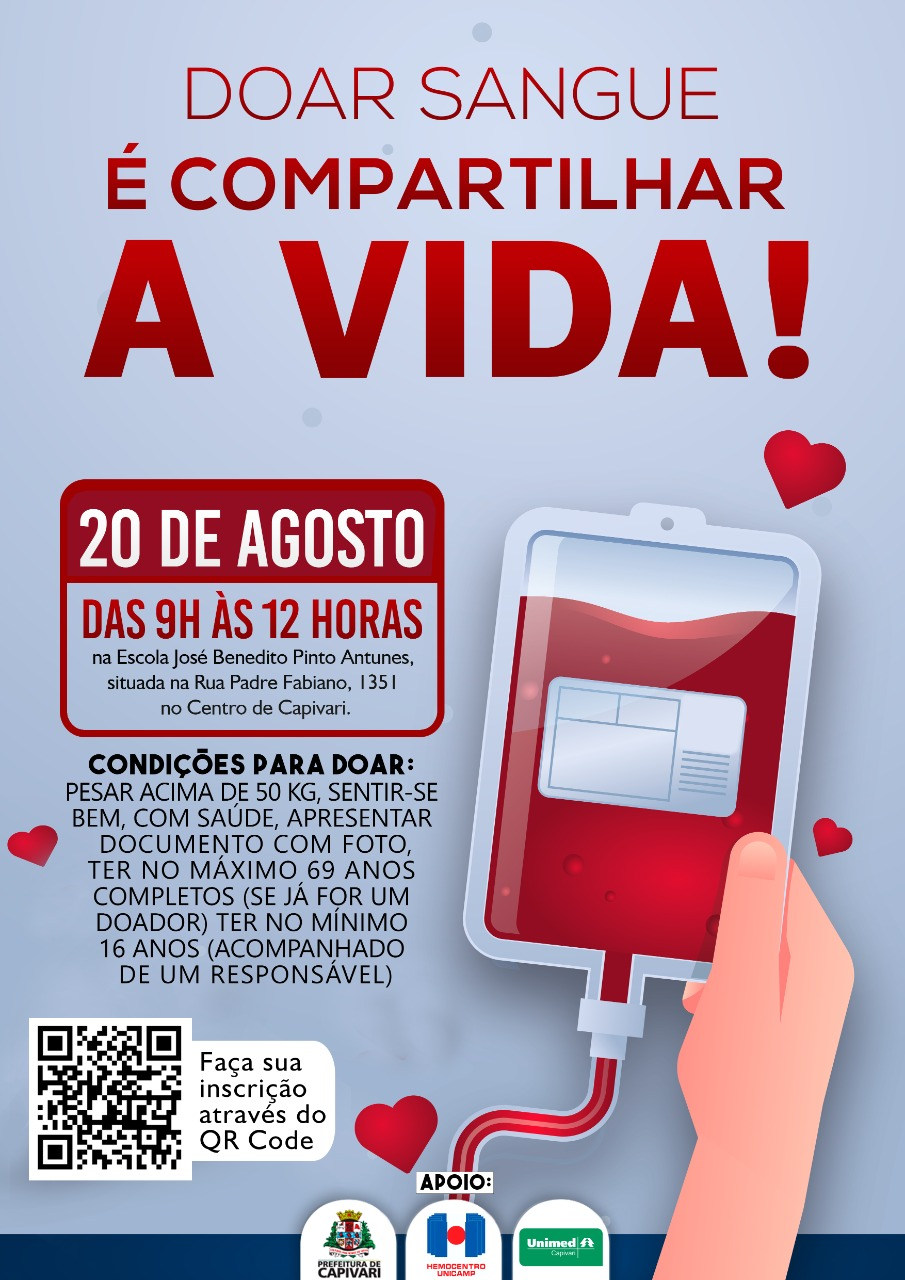
\includegraphics[width=5.76042in,height=8.15278in]{./imgSAEB_7_POR/media/image1.png} \\
\bottomrule
\end{longtable}

\fonte{Prefeitura de Capivari. Secretaria de Saúde anuncia Campanha de Doação de Sangue no dia 20 de agosto. Disponível em:
https://capivari.sp.gov.br/portal/secretaria-de-saude-anuncia-campanha-de-doacao-de-sangue-no-dia-20-de-agosto/
Acesso em: 19 mai. 2023.}

\num{1} A imagem acima representa uma campanha de conscientização. Sabendo que se trata de um texto informativo que tem como objetivo sensibilizar o público, aponte quais os recursos não verbais contribuem para a persuasão.

\linhas{4}
\coment{O uso da imagem da bolsa de sangue sendo segurada como um celular
complementa a escolha da palavra ``compartilhar'' como recursos de persuasão
e sensibilização.}

\num{2} Encontre no texto o verbo que indica uma recomendação de mudança de atitude.
Escreva-o abaixo

\linhas{2}
\coment{Doar, compartilhar. O uso do verbo no infinitivo é uma característica do
gênero. Para incentivar uma atitude, estes tipos de texto utilizam de
linguagem apelativa e multimodal.}

\num{3} Assinale com (V) verdadeiro ou (F) falso as afirmações a seguir sobre os textos
de gênero jornalístico e midiático:

\begin{itemize}

( ) Apresentam linguagem direta

( ) É comum o uso de verbos no imperativo

( ) Servem para divulgar conhecimentos

( ) Tem como objetivo convencer ou informar

\end{itemize}

\coment{V, V, F, V}

Leia o seguinte trecho do Estatuto da Criança e do Adolescente --- ECA.

\begin{quote}
O PRESIDENTE DA REPÚBLICA: Faço saber que o Congresso Nacional decreta e
eu sanciono a seguinte Lei: (\ldots{})

Título II: Dos Direitos Fundamentais (\ldots{})

Capítulo II: Do Direito à Liberdade, ao Respeito e à Dignidade (\ldots{})

Art. 16. O direito à liberdade compreende os seguintes aspectos:

I --- ir, vir e estar nos logradouros públicos e espaços comunitários,
ressalvadas as restrições legais;

II --- opinião e expressão;

III --- crença e culto religioso;

IV --- brincar, praticar esportes e divertir-se;

V --- participar da vida familiar e comunitária, sem discriminação;

VI --- participar da vida política, na forma da lei;

VII --- buscar refúgio, auxílio e orientação. \\

\end{quote}

\fonte{Ministério dos Direitos Humanos e da Cidadania. O Estatuto da Criança e 
do Adolescente -- ECA. Disponível em:
http://www.gov.br/mdh/pt-br/navegue-por-temas/crianca-e-adolescente/publicacoes/o-estatuto-da-crianca-e-do-adolescente. Acesso em: 19 mai. 2023.}

\num{4} Analise a forma composicional do texto e identifique as características que
indicam que ele pertence à esfera jurídica.

\linhas{4}
\coment{As características que indicam que o texto pertence à esfera jurídica são as
seguinte: divisão em artigos e capítulos, uso de numerais romanos, uso de
linguagem formal, verbos no infinitivo.}

\num{5} O uso do verbo no infinitivo em textos jurídicos e legais tem uma função. 
Que função é essa?

\linhas{4}
\coment{Os verbos no infinitivo, no caso de textos de regulamentação, indicam
orientação, têm uma função de persuadir, convencer ou convidar a uma
ação ou atitude.}

\num{6} Analise o texto a seguir e responda às questões a respeito dele. 

% Suprimi essa imagem porque ela não tem grande contribuição para o material. Rogério, 19/5/23, 16h21
%\begin{longtable}[]{@{}
%>{\raggedright\arraybackslash}p{(\columnwidth - 0\tabcolsep) * \real{0.9861}}@{}}
%\toprule
%\endhead
%\textbf{Alerta importante para você que é jovem e vai ler esta cartilha}
\includegraphics[width=1.625in,height=3.36458in]{./imgSAEB_7_POR/media/image2.png}

\begin{quote}
O Estatuto da Criança e do Adolescente -- ECA -- proíbe a venda de
qualquer tipo de bebida alcoólica para menores de 18 anos.

Portanto, fique esperto!

Se alguém lhe oferecer, mesmo que gratuitamente, qualquer bebida
alcoólica, NÃO ACEITE!

Essa pessoa estará cometendo um crime.

É bom lembrar que o uso do álcool pode levar ao alcoolismo, uma doença
grave que atinge 12,3\% da população brasileira com idade entre 12 e 65
anos.

Entre os jovens de 12 a 17 anos, a taxa de alcoolismo é de 7\%.

Considere que este nível representa 554.000 jovens com sérios problemas
sociais e de saúde.

\end{quote}

\fonte{Portal do Professor do Ministério da Educação. Drogas: Cartilha Álcool e Jovens. 
Disponível em: http://portaldoprofessor.mec.gov.br/storage/materiais/0000011863.pdf.
Acesso em: 2 de abri de 2023.}

\begin{escolha}
  \item A quem se destina este texto? Copie do texto um trecho que justifique
  sua resposta.

\linhas{2}
\coment{O texto se destina a jovens, como se pode verificar por meio do trecho 
``Alerta importante para você que é jovem e vai ler esta cartilha''.}

  \item Releia a frase: ``Considere que este nível representa 554.000 jovens
  com sérios problemas sociais e de saúde.''. Ao utilizar o número que
  representa 7\% da população jovem, o autor traz uma nova informação.
  Qual o sentido de trazer esse número para o texto?

\linhas{4}
\coment{Ao apresentar o número de jovens que sofrem com problemas de alcoolismo, a
informação diz respeito direta e explicitamente ao público-alvo do texto, de modo 
a sensibilizá-lo.}

\end{escolha}

\num{7} No que diz respeito à linguagem, cite duas características comuns aos gêneros
jornalístico e de divulgação científica.

\coment{Tanto no texto jornalístico quanto no de divulgação científica a
linguagem empregada deve ser clara e objetiva e pode haver o uso de
recursos não verbais tais como imagens, gráficos, tabelas.} 

Leia o texto abaixo e responda as questões

\begin{quote}

\emph{Brasília, 23 de março de 2020}

Excelentíssimos(as) senhores(as), Presidente da República, Ministros de
Estado, Governadores(as), Prefeitos(as), Secretários(as) de Saúde e
gestores(as) do SUS,

O CNS, enquanto órgão responsável pelo controle social no SUS, orienta
que todos(as) os(as) referidos(as) nesta carta adotem medidas
emergenciais, em todas as unidades da federação, para os próximos dois
meses (abril e maio), visando conter a crise de Saúde que vivemos hoje e
que pode se agravar nos próximos dias. O objetivo é zelar pela
integridade física e mental dos cidadãos e cidadãs brasileiros, buscando
também ações específicas e sensíveis à realidade de pessoas em regime
carcerário ou cumprindo medidas socioeducativas, dentre outras
populações vulneráveis. (\ldots{})

\emph{Conselho Nacional de Saúde} 

\end{quote} 

\fonte{Conselho Nacional de Saúde. Carta aberta do CNS às autoridades 
brasileiras no enfrentamento ao Novo Coronavírus. Disponível em: https://conselho.saude.gov.br/ultimas-noticias-cns/1074-carta-aberta-do-cns-as-autoridades-brasileiras-no-enfrentamento-ao-novo-coronavirus.
Acesso em: 19 mai. 2023.}

\num{8} A quem se destina a carta?

\linhas{2}
\comente{A carta se destina ao Presidente da República, Ministros de Estado, Governadores (as),
Prefeitos(as), Secretários(as) de Saúde e gestores(as) do SUS.}

\num{9} Selecione do texto um trecho que expressa o motivo de reivindicação da carta.

\linhas{6}
\coment{O trecho que expressa o motivo de reivindicação da carta é ``O CNS, enquanto órgão
responsável pelo controle social no SUS, orienta que todos(as) os(as) referidos(as) nesta
carta adotem medidas emergenciais, em todas as unidades da federação, para os próximos dois
meses (abril e maio), visando conter a crise de Saúde que vivemos hoje e que pode se agravar
nos próximos dias. Nesse sentido, é fundamental que sejam potencializadas ou desenvolvidas as
seguintes ações''. 

\num{10} Relacione os textos e suas características.

% Please add the following required packages to your document preamble:
% \usepackage[table,xcdraw]{xcolor}
% If you use beamer only pass "xcolor=table" option, i.e. \documentclass[xcolor=table]{beamer}
\begin{table}[]
\begin{tabular}{|
>{\columncolor[HTML]{DAE8FC}}l |
>{\columncolor[HTML]{ECF4FF}}c |}
\hline
\textbf{(1) Petição} & (   ) É um texto argumentativo de reivindicação \\ \hline
\textbf{(2) Estatuto} & (   ) Tem como objetivo divulgar informações \\ \hline
\textbf{(3) Folheto} & (   ) Utiliza recursos não verbais como forma de persuasão \\ \hline
\textbf{(4) Notícia} & (   ) Tem por objetivo regulamentar e normatizar \\ \hline
\end{tabular}
\end{table}

\coment{(1) É um texto argumentativo de reivindicação. (4) Tem como objetivo divulgar informações.
(3) utiliza recursos não verbais como forma de persuasão. (2) tem por objetivo regulamentar e
normatizar.}

\colorsec{Treino}

\num{1}

\begin{quote}

De acordo com o professor José Carlos Farah, as quedas em idosos são comuns 
porque o processo de envelhecimento traz algumas perdas importantes no nosso corpo.
A osteopenia, que é a perda de massa óssea, deixa o osso enfraquecido,
e a perda da massa muscular, como consequência, traz a falta do controle
do movimento e equilíbrio, a perda cognitiva, que diminui a nossa
atenção e percepção e a baixa aptidão física''. Ainda segundo o
colunista, o processo de perdas do envelhecimento é inevitável. Mas
alguns hábitos podem ajudar e ele cita entre estes a prática da
atividade física. ``Os benefícios da prática da atividade física se
contrapõem ao processo de envelhecimento. O exercício promove o aumento
da massa muscular e da coordenação motora, do equilíbrio e das funções
cognitivas. Este hábito já diminui a possibilidade de quedas, associado
ao ambiente livre de possíveis obstáculos que podem atrapalhar o dia a
dia do idoso''. 

\end{quote}

\fonte{José Carlos Simon Farah. Jornal da USP. Exercícios físicos podem contribuir 
para a redução da queda de idosos. Disponível em: https://jornal.usp.br/radio-usp/exercicios-fisicos-podem-contribuir-para-a-reducao-da-queda-de-idosos/.
Acesso em: 3 abr. 2023. com adaptações.}

Pode-se afirmar que o trecho acima pertence a um texto de divulgação científica, pois contém:

\begin{escolha}
  
  \item informações técnicas voltadas ao público especializado da área médica.
  
  \item explicações de especialista sobre os benefícios do exercício físico para idosos.
  
  \item citações diretas de artigos científicos sobre benefícios do exercício físico.
  
  \item narrativas pessoais sobre osteopenia em idosos e benefícios do exercício físico..

\end{escolha}

\coment{SAEB: Identificar elementos constitutivos de gêneros de divulgação
científica.

BNCC: EF69LP02 -- Analisar e comparar peças publicitárias variadas
(cartazes, folhetos, outdoor, anúncios e propagandas em diferentes
mídias, spots, jingle, vídeos etc.), de forma a perceber a articulação
entre elas em campanhas, as especificidades das várias semioses e
mídias, a adequação dessas peças ao público-alvo, aos objetivos do
anunciante e/ou da campanha e à construção composicional e estilo dos
gêneros em questão, como forma de ampliar suas possibilidades de
compreensão (e produção) de textos pertencentes a esses gêneros.

a) Incorreta. Embora o texto contenha alguns vocábulos ligados à área médica, não se pode 
afirmar que as informações veiculadas sejam voltadas apenas ao público especializado.
b) Correta. O texto contém explicações sobre os benefícios do exercício físico para idosos.
c) Incorreta. O texto não contém citações de artigos científicos. Há apenas falas curtas de um
especialista no assunto.
d) Incorreta. O texto não contém narrativas pessoais sobre os processos inerentes ao envelhecimento.}

\num{2}

Analise os dois textos a seguir.

\begin{quote}

\textbf{TEXTO 1: ES registra aumento de casos de dengue na 1ª semana de janeiro}

\textit{Em todo o mês de janeiro de 2022, o Espírito Santo teve 951
casos. Só nesta primeira semana já foram 1.453. Infectologista acredita
que estado pode estar vivendo uma epidemia de casos da doença.}

Só na primeira semana do ano foram registrados 1.453 casos da dengue no
Espírito Santo. Número bem maior do que os registros do mês de janeiro
de 2022, quando no mês todo foram registrados 951 casos da doença.

Segundo o infectologista Crispim Cerutti, o estado pode estar vivendo
uma epidemia da doença.

``A gente tem epidemias que ocorrem a aproximadamente a cada três anos. A
última que a gente teve foi em 2019/2020. Embora o intervalo seja um
pouco curto, a gente pode dizer que sim, estamos em uma nova epidemia da
doença. A frequência de casos acompanha o ciclo de vida dos mosquitos'',
explicou o infectologista.

\end{quote}

\fonte{Naiara Arpini. G1. ES registra aumento de casos de dengue na 1ª semana de janeiro.
Disponível em: https://g1.globo.com/es/espirito-santo/noticia/2023/01/18/es-registra-aumento-de-casos-de-dengue-na-1a-semana-de-janeiro.ghtml. Acesso em:
19 mai. 2023.}

\textbf{Exemplo 2: Como eu posso ajudar?}

Para evitar a reprodução do Aedes aegypti, o Ministério da Saúde reúne
uma série de orientações à população. Confira abaixo:

\begin{itemize}
  
  \item Utilize telas de proteção com buracos de, no máximo, 1,5 milímetros nas
janelas de casa;
  
  \item Deixe as portas e janelas fechadas, principalmente nos períodos do nascer e do pôr do sol;
  
  \item Mantenha o terreno limpo e livre de materiais ou entulhos que possam ser criadouros;
  
  \item Tampe os tonéis e caixas d'água;
  
  \item Mantenha as calhas limpas;
  
  \item Deixe garrafas sempre viradas com a boca para baixo;
  
  \item Mantenha lixeiras bem tampadas;
  
  \item Deixe ralos limpos e com aplicação de tela;
  
  \item Limpe semanalmente ou preencha pratos de vasos de plantas com areia;
  
  \item Limpe com escova ou bucha os potes de água para animais;
  
  \item Limpe todos os acessórios de decoração que ficam fora de casa e evite o acúmulo de água em pneus e calhas;
  
  \item Coloque repelentes elétricos próximos às janelas -- o uso é contraindicado para pessoas alérgicas;
  
  \item Velas ou difusores de essência de citronela também podem ser usados;
  
  \item Evite produtos de higiene com perfume, pois podem atrair insetos;
  
  \item Retire água acumulada na área de serviço, atrás da máquina de lavar
  roupa.
 
\end{itemize}

\fonte{Helio Carvalho. G1. Sete cidades da região de Campinas vivem situação de alerta para dengue; entenda o que significa.
Disponível em: https://g1.globo.com/sp/campinas-regiao/noticia/2023/01/17/sete-cidades-da-regiao-de-campinas-vivem-situacao-de-alerta-para-dengue-entenda-o-que-significa.ghtml. 
Acesso em: 19 mai. 2023.}

Os dois exemplos foram retirados de veículos de imprensa e tratam de
questões relacionadas à dengue. Quanto às diferenças e semelhanças entre
os dois exemplos, assinale a alternativa correta:

\begin{escolha}

\item Os dois exemplos pretendem informar a população sobre como evitar os casos de dengue.

\item O primeiro apresenta uma notícia, e o segundo traz indicações de ações de prevenção.

\item O primeiro exemplo é um texto de opinião; o segundo, um folheto informativo.

\item O primeiro texto traz dados científicos sobre a dengue e o segundo é um texto instrucional.

\end{escolha}

\voment{SAEB:Analisar a relação temática entre diferentes gêneros jornalísticos.

a) Incorreta. O primeiro exemplo traz uma notícia sobre o número de casos
e segundo exemplo traz indicações de ações para prevenir a
proliferação do mosquito.

b) Correta. O primeiro exemplo é uma
notícia sobre o número de casos de dengue em 2023; o segundo contém
indicações de ações de prevenção e combate à proliferação do
mosquito que transmite a doença.

c) Incorreta. Embora o segundo exemplo possa ser considerado um texto
informativo, o primeiro exemplo não é um texto de opinião.

d) Incorreta. O primeiro exemplo não traz dados científicos e nem possui
linguagem científica e técnica sobre o assunto.}

\num{3}

Leia os trechos extraídos da constituição Brasileira de 1988 e responda
o que se pede:

Trecho 1:

\begin{quote}

\textbf{Trecho 1}

Art. 1.º A República Federativa do Brasil, formada pela união
indissolúvel dos Estados e Municípios e do Distrito Federal,
constitui-se em Estado democrático de direito e tem como fundamentos: (\ldots{})

Art. 3.º Constituem objetivos fundamentais da República Federativa do
Brasil:

IV - promover o bem de todos, sem preconceitos de origem, raça, sexo,
cor, idade e quaisquer outras formas de discriminação.

Art. 4.º A República Federativa do Brasil rege-se nas suas relações
internacionais pelos seguintes princípios:

III - autodeterminação dos povos;

\end{quote}


\begin{quote}
\textbf{Trecho 2}

Art. 215. O Estado garantirá a todos o pleno exercício dos direitos
culturais e acesso às fontes da cultura nacional, e apoiará e
incentivará a valorização e a difusão das manifestações culturais.

§ 1.º O Estado protegerá as manifestações das culturas populares,
indígenas e afrobrasileiras, e das de outros grupos participantes do
processo civilizatório nacional. Art. 216. Constituem patrimônio
cultural brasileiro os bens de natureza material e imaterial, tomados
individualmente ou em conjunto, portadores de referência à identidade, à
ação, à memória dos diferentes grupos formadores da sociedade
brasileira, nos quais se incluem:

I - as formas de expressão;

II - os modos de criar, fazer e viver;

III - as criações científicas, artísticas e tecnológicas;

IV - as obras, objetos, documentos, edificações e demais espaços
destinados às manifestações artístico-culturais;

V - os conjuntos urbanos e sítios de valor histórico, paisagístico,
artístico, arqueológico, paleontológico, ecológico e científico.

§ 1.º O poder público, com a colaboração da comunidade, promoverá e
protegerá o patrimônio cultural brasileiro, por meio de inventários,
registros, vigilância, tombamento e desapropriação, e de outras formas
de acautelamento e preservação. \\

\end{quote}

\fonte{Constituição da República Federativa do Brasil. Disponível
em: https://www2.senado.leg.br/bdsf/bitstream/handle/id/518231/CF88_Livro_EC91_2016.pdf.
Acesso em: 19 mai. 2023.}

Sobre os trechos selecionados é correto afirmar que:

\begin{escolha}

  \item os dois trechos são contraditórios entre si.

  \item não há relação direta entre os dois trechos.

  \item os dois trechos versam sobre questões distintas.

  \item os dois trechos são complementares. 

\end{enumerate}

\coment{SAEB: Identificar formas de organização de textos normativos, legais
e/ou reivindicatórios.

BNCC: EF69LP27 -- Analisar a forma composicional de textos
pertencentes a gêneros normativos/ jurídicos e a gêneros da esfera
política, tais como propostas, programas políticos (posicionamento
quanto a diferentes ações a serem propostas, objetivos, ações previstas
etc.), propaganda política (propostas e sua sustentação, posicionamento
quanto a temas em discussão) e textos reivindicatórios: cartas de
reclamação, petição (proposta, suas justificativas e ações a serem
adotadas) e suas marcas linguísticas, de forma a incrementar a
compreensão de textos pertencentes a esses gêneros e a possibilitar a
produção de textos mais adequados e/ou fundamentados quando isso for
requerido.

a) Incorreta. Os trechos não são contraditórios. O segundo trecho
apenas trata de uma parcela da população em particular enquanto o
primeiro trata do conjunto da população brasileira.

b) Incorreta. Os trechos apresentam relação direta ao passo que a
população indígena faz parte da população brasileira e como tal também
tem direitos civis garantidos pela lei.

c) Incorreta. Os dois trechos versam sobre direitos essenciais, portanto
não tratam de questões distintas.

d)Correta. Os dois trechos apresentam relação de complementaridade, pois
as disposições presentes no segundo trecho apenas especificam direitos
dos povos indígenas e deveres do Estado brasileiro para com essa
população a fim de garantir as obrigações do Estado brasileiro dispostas
no Artigo 3º.}

\chapter{Nas tramas do texto literário}
\markboth{Módulo 3}{}

\colorsec{Habilidades do SAEB}

\begin{itemize}
  
  \item Analisar elementos constitutivos de textos pertencentes ao domínio literário.
  
  \item Analisar a intertextualidade entre textos literários ou entre estes e outros textos 
verbais ou não verbais.
  
  \item Inferir a presença de valores sociais, culturais e humanos em textos literários.

\end{itemize}

\colorsec{Habilidades da BNCC}

\begin{itemize}

  \item EF69LP44, EF69LP47, EF67LP27

\end{itemize}

\conteudo{A literatura, assim como todo o escopo das artes, é uma poderosa
ferramenta de expressão de crenças, valores e ideias de determinada
sociedade. Por meio de textos literários são apreendidos os hábitos, os
acontecimentos, desafios e questões de determinada época. Alguns textos
literários são tão ricos e tratam de temas tão essenciais e universais
que acabam por sobreviver ao tempo. Para além do texto escrito, as
narrativas verbais também servem como meio de eternização de certas
questões, sentimentos e desafios enfrentados pelos seres humanos. Não
por acaso, marcas de intertextualidade permeiam a cultura literária. Em
obras literárias é possível entrever, de forma direta ou indireta, as
relações com outros tipos de arte, verbais e não verbais. A análise dos
elementos constitutivos das produções literárias permite perceber as
características e singularidades para compreender o porquê de algumas
obras serem tão singulares. Elementos tais como enredo e linguagem podem
dizer muito sobre determinados grupos, culturas e épocas. Portanto, a análise dos
aspectos constitutivos dos textos literários e suas narrativas pressupõe
um entendimento da literatura que ultrapassa seu valor estético e dota
de sentido filosófico, sociológico, histórico e antropológico a produção
textual artística. Por isso, é fundamental o estudo de aspectos pertinentes à
linguagem, ao estilo, à estrutura e à temática das narrativas. 
A Literatura tem o poder de despertar sensações,
questionamentos e proporcionar experiências estéticas que se refletem na
maneira como as pessoas escolhem ser e estar no mundo. O reconhecimento
do valor e da importância das obras do domínio literário pode
proporcionar uma formação ética e questionadora que participa da
formação cultural e intelectual da sociedade.}

\coment{Professor(a), questione os estudantes sobre os gêneros textuais
literários que conhecem, retome as principais características
do conto, crônica, poesia, literatura de cordel, romance e demais
gêneros que surgirem.

Reforce a ideia de que tais gêneros retratam a sociedade com seus
valores e desafios. Retome com os os estudantes os conhecimentos
prévios sobre mitos, lendas e demais textos de origem popular e saliente
a forma como os temas trabalhados remontam a hábitos, valores e crenças
da cultura e da época em que foram escritos (lenda do milho, da
mandioca, do arroz, sobre os rios, a paisagem, ritos de passagem,
comemorações, etc). Chame a atenção dos estudantes para o
fato de que os diversos tipos de artes podem se comunicar. Neste caso,
pode ser citado como exemplo o texto dramático --- que
pode ser lido, mas é escrito para ser encenado. Mostre como o teatro
também promove integração de diversas expressões artísticas. Cite também
outras expressões tais como a música e as artes plásticas e estimule os
estudantes a pensarem como essas expressões se complementam.}

\colorsec{Atividades}

\num{1} O conto popular é um gênero literário proveniente da tradição oral e em sua textualidade mantém algumas marcas de estilo quanto à linguagem. Sobre este aspecto da linguagem dos contos populares, cite duas marcas fundamentais deste gênero.

\coment{O gênero conto popular é marcado pela linguagem simples, direta e com
fortes traços de oralidade tais como regionalismos, gírias e expressões
populares.}

\num{2} Textos narrativos curtos e objetivos, baseados em eventos do cotidiano: este gênero textual tem como objetivo divertir, entreter, provocar reflexão ou fazer uma crítica. Qual gênero literário possui essas características?

\coment{As características apresentadas se referem à crônica, que traz questões 
cotidianas e pode conter traços de humor.}

Leia o trecho a seguir e responda as questões:

\begin{verse}

Disse Pedro isso é blasfêmia \\

É bastante astucioso \\

Pistoleiro e cangaceiro \\ 

Esse povo é impiedoso \\

Não ganharão o perdão \\

Do santo Pai Poderoso 


Inda mais tem sua má fama \\

Vez por outra comentada \\

Quando há um julgamento \\

Duma alma tão penada \\

Porque fora violenta \\

Em sua vida é baseada. 

\end{verse}

\fonte{Guaipuan Vieira. A chegada de lampião no céu. Disponível em: http://www.dominiopublico.gov.br/download/texto/rd000001.pdf.
Acesso em: 20 mai. 2023.}

\num{3} O texto acima pertence a qual gênero textual?

\linhas{1}
\coment{O texto pertence à Literatura de Cordel.}

\num{4} Cite duas características do gênero presentes no trecho.

\linhas{4}
\coment{Divisão em estrofes e versos, rima, métrica, temas da cultura
nordestina, no caso o personagem Lampião, marcas de oralidade.}

\num{5} Use a legenda para indicar as características da crônica e do conto.
Marque (1) para o crônica e (2) para o conto. Os dois podem ter
características em comum:

% Please add the following required packages to your document preamble:
% \usepackage[table,xcdraw]{xcolor}
% If you use beamer only pass "xcolor=table" option, i.e. \documentclass[xcolor=table]{beamer}
\begin{table}[]
\begin{tabular}{|
>{\columncolor[HTML]{DAE8FC}}l |l|}
\hline
 & Poucos personagens \\ \hline
 & Curto e objetivo \\ \hline
 & Histórias narram fatos do cotidiano e podem estimular a reflexão \\ \hline
 & Podem surgir de narrativas populares transmitidos pela tradição oral \\ \hline
 & É comum que seja publicado em jornais \\ \hline
\end{tabular}
\end{table}

\coment{
% Please add the following required packages to your document preamble:
% \usepackage[table,xcdraw]{xcolor}
% If you use beamer only pass "xcolor=table" option, i.e. \documentclass[xcolor=table]{beamer}
\begin{table}[]
\begin{tabular}{|
>{\columncolor[HTML]{DAE8FC}}c |l|}
\hline
1, 2 & Poucos personagens \\ \hline
1, 2 & Curto e objetivo \\ \hline
1 & Histórias narram fatos do cotidiano e podem estimular a reflexão \\ \hline
2 & Podem surgir de narrativas populares transmitidos pela tradição oral \\ \hline
1 & É comum que seja publicado em jornais \\ \hline
\end{tabular}
\end{table}
}

Leia o trecho a seguir e responda.

\begin{quote}

Houve noutro tempo um rei que tinha o hábito de jogar, e todos com
quem jogava perdiam. Uma vez convidou a um outro rei para jogar, e, no
dia marcado, este se apresentou; mas perdeu todas as mãos do jogo, até
que se desenganou e despediu-se para se ir embora.

\end{quote}

\fonte{Sílvio Romero. Contos Populares do Brasil. Coleção acervo brasileiro.
Volume 3, 2ª edição. Jundiaí: Cadernos do mundo inteiro, 2018 p. 128.}

\num{6} O que a expressão ``Houve noutro tempo'' quer dizer? Comumente outra
expressão é usada para iniciar os contos. Que expressão é essa?

\linhas{3}
\coment{A expressão faz alusão a um tempo passado indeterminado. Nos contos é
comum que apareça a expressão ``Era uma vez'' com o mesmo significado de
tempo indeterminado.}

\num{7} Com base no trecho acima, indique qual o tipo de narrador.

\linhas{3}
\coment{Com base no trecho, podemos dizer que o tipo de narrador é o
narrador observador.}

\num{8} Sobre a intertextualidade presente nas artes em geral, e em específico
na literatura, assinale verdadeiro (V) ou falso (F) para as seguintes
afirmações.

% Please add the following required packages to your document preamble:
% \usepackage[table,xcdraw]{xcolor}
% If you use beamer only pass "xcolor=table" option, i.e. \documentclass[xcolor=table]{beamer}
\begin{table}[]
\begin{tabular}{|
>{\columncolor[HTML]{DAE8FC}}c |l|}
\hline
 & É a prática de copiar trechos de outras obras \\ \hline
 & \begin{tabular}[c]{@{}l@{}}É um recurso que pode trazer ainda mais possibilidades de\\ interpretação para um texto\end{tabular} \\ \hline
 & \begin{tabular}[c]{@{}l@{}}Pode estar implícita ou explícita em textos e demais obras\\ artísticas\end{tabular} \\ \hline
 & Pode estar presente em traduções, paródias e releituras de obras \\ \hline
 & Pode ser caracterizada como plágio \\ \hline
\end{tabular}
\end{table}

\coment{F, V, V, V, F}

\num{9} No trecho abaixo vemos um exemplo de discurso indireto:

\begin{quote}

O pai explicou: 
--- Filha, você precisa fazer sua tarefa agora. Mais tarde
temos compromisso.

\end{quote}

Passe a frase para o discurso indireto.

\coment{O pai explicou para a filha que ela precisava fazer a tarefa naquele
momento, pois, mais tarde, eles tinham compromisso.}

\colorsec{Treino}

\num{1}

\begin{quote}

\textbf{Lenda da Mandioca}

\emph{Lenda Indígena}

Era uma vez uma índia chamada Atiolô. Quando o chão começou a ficar
coberto de frutinhas de murici, ela se casou com Zatiamarê. As frutinhas
desapareceram, as águas do rio subiram apodrecendo o chão. Depois, o sol
queimou a terra, um ventinho molhado começou a chegar do alto da serra.
Quando os muricis começaram outra vez a cair, numa chuvinha amarela,
Atiolô começou a rir sozinha. Estava esperando uma menininha.

\end{quote}

\fonte{Ana Rosa Abreu e outros autores. Contos tradicionais, fábulas,
lendas e mitos. Disponível em http://www.dominiopublico.gov.br/download/texto/me001614.pdf. Acesso em: 20 mai. 2023)}

Nesse trecho da lenda da mandioca, notam-se traços da cultura
indígena com relação ao modo de explicar a origem dos alimentos, a
origem da natureza, a preservação dos costumes e a contagem do tempo.
Pode-se notar que a fruta murici é indicadora da passagem de certo 
período de tempo. Assinale a alternativa que explica corretamente 
quanto tempo se passou.

\begin{escolha}

  \item É possível inferir que cerca de um ano se passou.
  
  \item Não se pode saber ao certo quanto tempo se passou.
  
  \item A mudança de estação indica a passagem de três meses.  
  
  \item É legítimo pressupor que muitos anos se passaram. 

\end{escolha}

\coment{SAEB: Inferir a presença de valores sociais, culturais e humanos em
textos literários.

BNCC: EF69LP44 -- Inferir a presença de valores sociais,
culturais e humanos e de diferentes visões de mundo, em textos
literários, reconhecendo nesses textos formas de estabelecer múltiplos
olhares sobre as identidades, sociedades e culturas e considerando a
autoria e o contexto social e histórico de sua produção.

a) Correta. O trecho faz alusão à passagem das quatro estações do ano
exemplificadas pelo ciclo natural da fruta murici, além de referir-se
a períodos de seca e cheia, que permitem inferir a passagem de cerca de um ano.
b) Incorreta. Por meio das características citadas, tais como ocorrência
de chuvas e seca, pode-se inferir que um ano se passou.
c) Incorreta. O trecho faz alusão a diversas características das estações
do ano, portanto mais de uma estação se passou, indicando a passagem
de um ano.
d) Incorreta. O trecho faz alusão à passagem das quatro estações do ano
exemplificadas pelo ciclo natural da fruta murici, além de referir-se
a períodos de seca e cheia, que permitem inferir a passagem de cerca de um ano.}

\num{2}

Leia os poemas abaixo e responda:

\textbf{Texto I: Canção do exílio}

\emph{Gonçalves Dias}

\begin{verse}

Minha terra tem palmeiras, \\

Onde canta o Sabiá; \\

As aves, que aqui gorjeiam, \\

Não gorjeiam como lá. 


Nosso céu tem mais estrelas,\\

Nossas várzeas têm mais flores, \\

Nossos bosques têm mais vida, \\

Nossa vida mais amores.


Em cismar, sozinho, à noite, \\

Mais prazer eu encontro lá; \\

Minha terra tem palmeiras, \\

Onde canta o Sabiá. \\


Minha terra tem primores, \\

Que tais não encontro eu cá; \\

Em cismar -- sozinho, à noite -- \\

Mais prazer eu encontro lá; \\

Minha terra tem palmeiras, \\

Onde canta o Sabiá. 


Não permita Deus que eu morra, \\

Sem que eu volte para lá; \\

Sem que desfrute os primores \\

Que não encontro por cá; \\

Sem qu'inda aviste as palmeiras, \\

Onde canta o Sabiá.

\end{verse}

\end{quote}

\fonte{Gonçalves Dias. Primeiros Cantos. Disponível em:
http://www.dominiopublico.gov.br/download/texto/bn000100.pdf.
Acesso em: 6 abr de 2023.}



\begin{quote}

\textbf{Texto II: Canção do exílio}

\emph{Murilo Mendes}

\begin{verse}

Minha terra tem macieiras da Califórnia \\

onde cantam gaturamos de Veneza. \\

Os poetas da minha terra \\

são pretos que vivem em torres de ametista, \\

os sargentos do exército são monistas, cubistas, \\

os filósofos são polacos vendendo a prestações. {[} \ldots{} {]} \\

Ai quem me dera chupar uma carambola de verdade \\

e ouvir um sabiá com certidão de idade!

\end{verse}

\end{quote}

\fonte{Murilo Mendes. Poesias. Rio de Janeiro: José Olympio, 1959.}

A primeira versão, escrita por Gonçalves Dias em 1847, tornou-se
importante obra representante do romantismo. Posteriormente, em 1930, o
poeta modernista Murilo Mendes retomou a poesia de Gonçalves Dias e
criticou as influências estrangeiras na cultura brasileira
apropriando-se do nacionalismo do Romantismo, transpondo-o para o
nacionalismo modernista. Sobre esta relação de
intertextualidade em obras literárias assinale a alternativa correta.

\begin{escolha}

  \item O poema de Murilo Mendes é um plágio do poema de Gonçalves Dias.

  \item O poema de Murilo Mendes não se refere ao poema de Gonçalves Dias.

  \item O poema de Murilo Mendes é uma paródia do poema de Gonçalves Dias.

  \item O poema de Gonçalves Dias é uma paródia do poema de Murilo Mendes.

\end{escolha}

\coment{SAEB: Analisar a intertextualidade entre textos literários ou entre
estes e outros textos verbais ou não verbais.

BNCC: EF67LP27 -- Analisar, entre os textos literários e entreestes e outras manifestações artísticas (como cinema, teatro, música,
artes visuais e midiáticas), referências explícitas ou implícitas a
outros textos, quanto aos temas, personagens e recursos literários e
semióticos

a) Incorreta. Os traços de intertextualidade não se configuram como plágio.
b) Incorreta. Além do título, existem diversas alusões de Murilo Mendes ao 
poema de Gonçalves Dias.
c) Correta. O tipo de intertextualidade entre os dois poemas é chamado de
paródia, que pode satirizar, de criticar ou de homenagear o texto de referência.
Neste caso, Murilo Mendes critica o nacionalismo no Romantismo
brasileiro e junto ao movimento modernista propõe uma nova forma de
nacionalismo que valoriza a cultura brasileira.
d)  O poema de Gonçalves Dias foi escrito cerca de 100 anos antes,
portanto não pode ser baseado no poema de Murilo Mendes.}

\num{3}


\includegraphics[width=4.11458in,height=2.80208in]{./imgSAEB_7_POR/media/image3.png}

\fonte{OBRANOME. Catálogo. Caixa Econômica Federal e
Embaixada da Espanha, no Conjunto Cultural da Caixa, Brasília 2003.}

O poema acima pode ser caracterizado como um poema visual. Os poemas
visuais foram amplamente explorados pelos poetas do concretismo e contêm características próprias. Sobre as características da poesia
concreta, assinale a alternativa correta.

\begin{escolha}

  \item A combinação de palavras e imagens é irrelevante para a criação dos sentidos do poema. 

  \item Regras rígidas para a estrutura em versos rimados e estrofes 
  caracterizam a poesia visual.

  \item Imagens ilustrativas não têm relação com os sentidos propostos 
  pelo autor.

  \item A disposição de letras e palavras na página é recurso de produção de sentidos do poema.

\end{escolha}

\coment{SAEB: Analisar elementos constitutivos de textos pertencentes ao domínio
literário.

a) Incorreta. Na poesia concreta, pode haver combinação de palavras e imagens 
para a criação dos sentidos do poema.
b) Incorreta. Não se verificam versos rimados e estrofes tradicionais na poesia
visual. 
c) Incorreta. As imagens podem fazer parte da constituição do poema e contribuir
para a produção de sentido.
d) Correta. A disposição de letras e palavras na página é, de fato, recurso de
produção de sentidos do poema.}

\chapter{Formas de composição do sentido}
\markboth{Módulo 4}{}

\colorsec{Habilidades do SAEB}

\begin{itemize}
  
  \item Analisar efeitos de sentido produzido pelo uso de formas de apropriação 
  textual (paráfrase, citação etc.).
  
  \item Analisar os efeitos de sentido decorrentes dos mecanismos de construção 
  de textos jornalísticos/midiáticos.

\end{itemize}


\colorsec{Habilidades da BNCC}

\begin{itemize}

  \item EF69LP16, EF69LP43.

\end{itemize}

\conteudo{Há muitos elementos utilizados para argumentação em textos.
Por meio da estrutura do texto, da escolha de palavras e de recursos de estilo,
é possível perceber objetivos e intenções do autor. Os textos argumentativos
-- tais como artigos de opinião, editoriais ou discursos -- apresentam em sua
construção elementos que visam convencer de alguma ideia ou expor determinado 
ponto de vista. Para atingir esse objetivo, o autor se vale da coesão e da 
coerência. Com argumentos consistentes, bem concatenados e ideias claras, 
é possível encaminhar ao leitor as ideias almejadas. Existem recursos adequados
para persuadir ou convencer o
leitor: é o caso de argumentos de especialistas, dados de pesquisas ou exemplos,
entre muitos outros. Toda pessoa que deseja comunicar algo faz uso desses
recursos: no âmbito pessoal, em conversas informais entre colegas e familiares;
no âmbito profissional, em negociações e reuniões; no âmbito político, em
discursos; no âmbito estudantil e acadêmico, na elaboração de teses,
dissertações e apresentações de trabalho. Portanto, saber reconhecer e
utilizar recursos de persuasão e convencimento é fundamental para a 
convivência em sociedade e para a resolução de conflitos nos quais há a
necessidade discursos claros e orientados por argumentos. 

Para cada gênero textual, existem recursos comuns que auxiliam na boa
comunicação, de acordo com a finalidade e intenção do comunicador.
Dentre eles, o uso de aspas para introduzir citações, o uso de exemplos
para produzir argumentos, a escolha das palavras e de expressões de
acordo com o receptor.}

\coment{Professor(a), relembre os estudantes sobre a necessidade de persuasão e
convencimento nos gêneros textuais já estudados. É comum que relacionem
a persuasão aos textos publicitários, mas vá além e discuta recursos de
convencimento também em textos de opinião e em situações cotidianas.}

\colorsec{Atividades}

Leia o texto abaixo para responder as questões:

\begin{quote}

\textbf{Especialistas indicam formas de combate a atos de intimidação}

Um em cada dez estudantes brasileiros é vítima de bullying -- anglicismo
que se refere a atos de intimidação e violência física ou psicológica,
geralmente em ambiente escolar. O dado foi divulgado esta semana pelo
Programa Internacional de Avaliação de Estudantes (Pisa) 2015.

Especialistas, como a professora de psicologia Ciomara Shcneider,
psicanalista de crianças e adolescentes, defendem que pais e escola
devem estar atentos ao comportamento dos jovens e manter sempre abertos
os canais de comunicação com eles. Para ela, o diálogo continua a ser a
melhor arma contra esse tipo de violência, que pode causar efeitos
devastadores em crianças e adolescentes.

A Lei nº 13.185, em vigor desde 2016, classifica o bullying como
intimidação sistemática, quando há violência física ou psicológica em
atos de humilhação ou discriminação. A classificação também inclui
ataques físicos, insultos, ameaças, comentários e apelidos pejorativos,
entre outros.

``Os casos de bullying começam muito mais silenciosos e, por isso, são
mais graves. Quem sofre a agressão não conta nem na escola nem na
família, mas começa a mudar o comportamento'', explica. De acordo com
ela, queda no rendimento escolar, faltas na escola e mudanças no
comportamento são os sinais mais frequentes apresentados por quem sofre
esse tipo de violência. Por isso, família e escola devem estar sempre
atentos para os sinais que são apresentados pelos jovens.

Os mesmos cuidados, alerta a psicóloga, valem para situações enfrentadas
fora da escola, seja no mundo virtual -- como em casos de cyberbullying
--, na vizinhança onde moram ou nos locais que costumam frequentar.

\end{quote}

\fonte{Ministério da Educação. Bullying. Disponível 
em: http://portal.mec.gov.br/component/tags/tag/34487#. 
Acesso em: 20 mai. 2023.}

\num{1} Qual o principal assunto abordado no texto?

\linhas{1}
\coment{O assunto do texto é o bullying.}

\num{2} Cite um elemento do texto que traz maior confiabilidade às informações.

\linhas{3}
\coment{Discursos de autoridade, exemplos, dados de pesquisas e institutos de
pesquisa conferem credibilidade ao conjunto do texto e às informações nele 
contidas.}

\num{3} Qual a função do travessão no primeiro parágrafo do texto?

\linhas{1}
\coment{A função do travessão é explicar o termo bullying.}

\num{4} Transcreva do texto o trecho em que a especialista oferece recursos
para lidar contra esse tipo de violência. 

\linhas{5}
comnet{O trecho solicitado é ``Para ela, o diálogo continua a ser a melhor
arma contra esse tipo de violência, que pode causar efeitos devastadores em
crianças e adolescentes.''}

\num{5} Utilize a legenda para classificar os tipos de argumento selecionados:

% Please add the following required packages to your document preamble:
% \usepackage[table,xcdraw]{xcolor}
% If you use beamer only pass "xcolor=table" option, i.e. \documentclass[xcolor=table]{beamer}
\begin{table}[]
\begin{tabular}{|
>{\columncolor[HTML]{DAE8FC}}l |l|}
\hline
\textbf{(I) Argumento por Provas Concretas} & \begin{tabular}[c]{@{}l@{}}(     ) Especialistas, como a professora de psicologia Ciomara Shcneider,\\ psicanalista de crianças e adolescentes, defendem que pais e escola\\ devem estar atentos ao comportamento dos jovens e manter sempre abertos\\ os canais de comunicação com eles.\end{tabular} \\ \hline
\textbf{(II) Argumento de Autoridade} & \begin{tabular}[c]{@{}l@{}}(     ) Um em cada dez estudantes brasileiros é vítima de bullying -\\ anglicismo que se refere a atos de intimidação e violência física ou\\ psicológica, geralmente em ambiente escolar. O dado foi divulgado esta\\ semana pelo Programa Internacional de Avaliação de Estudantes (Pisa)\\ 2015.\end{tabular} \\ \hline
\textbf{(III) Argumento por Exemplificação} & \begin{tabular}[c]{@{}l@{}}(     ) A Lei nº 13.185, em vigor desde 2016, classifica o bullying como \\ intimidação sistemática, quando há violência física ou psicológica em\\ atos de humilhação ou discriminação. A classificação também inclui\\ ataques físicos, insultos, ameaças, comentários e apelidos pejorativos,\\ entre outros.\end{tabular} \\ \hline
\end{tabular}
\end{table}

\coment{% Please add the following required packages to your document preamble:
% \usepackage[table,xcdraw]{xcolor}
% If you use beamer only pass "xcolor=table" option, i.e. \documentclass[xcolor=table]{beamer}
\begin{table}[]
\begin{tabular}{|
>{\columncolor[HTML]{DAE8FC}}l |l|}
\hline
\textbf{(I) Argumento por Provas Concretas} & \begin{tabular}[c]{@{}l@{}}(II) Especialistas, como a professora de psicologia Ciomara Shcneider,\\ psicanalista de crianças e adolescentes, defendem que pais e escola\\ devem estar atentos ao comportamento dos jovens e manter sempre abertos\\ os canais de comunicação com eles.\end{tabular} \\ \hline
\textbf{(II) Argumento de Autoridade} & \begin{tabular}[c]{@{}l@{}}(I) Um em cada dez estudantes brasileiros é vítima de bullying -\\ anglicismo que se refere a atos de intimidação e violência física ou\\ psicológica, geralmente em ambiente escolar. O dado foi divulgado esta\\ semana pelo Programa Internacional de Avaliação de Estudantes (Pisa)\\ 2015.\end{tabular} \\ \hline
\textbf{(III) Argumento por Exemplificação} & \begin{tabular}[c]{@{}l@{}}(III) A Lei nº 13.185, em vigor desde 2016, classifica o bullying como \\ intimidação sistemática, quando há violência física ou psicológica em\\ atos de humilhação ou discriminação. A classificação também inclui\\ ataques físicos, insultos, ameaças, comentários e apelidos pejorativos,\\ entre outros.\end{tabular} \\ \hline
\end{tabular}
\end{table}
}

\num{6} Copie do texto o trecho em que a especialista explica outro tipo de violência associada ao bullying que ocorre fora da escola

\linhas{5}
\coment{O trecho solicitado é ``Os mesmos cuidados, alerta a psicóloga, valem
para situações enfrentadas fora da escola, seja no mundo virtual -- como em
casos de cyberbullying --, na vizinhança onde moram ou nos locais que costumam frequentar.}

\num{7} Qual o sinal usado para marcar as falas da especialista?

\linhas{1}
\coment{O sinal usado para marcar as falas da especialista são as aspas.}

\num{8} No trecho ``De acordo com ela, queda no rendimento escolar, faltas na
escola e mudanças no comportamento são os sinais mais frequentes
apresentados por quem sofre esse tipo de violência.'' O pronome \textbf{ela} se
refere a quem?

\linhas{1}
\coment{O pronome se refere à professora de psicologia Ciomara Shcneider.}

\num{9} A paráfrase é um recurso muito comum em textos de opinião e
argumentativos. Este recurso visa a reescrita de alguma fala ou
citação sem que seja necessária a referência direta. Retire do texto
um exemplo de paráfrase.

\linhas{4}
O trecho a seguir contém paráfrase: ``Para ela, o diálogo continua a ser a
melhor arma contra esse tipo de violência, que pode causar efeitos devastadores
em crianças e adolescentes.''}

\num{10} Reescreva em forma de paráfrase a seguinte fala da especialista: ``Os 
casos de bullying começam muito mais silenciosos e, por isso, são mais graves. 
Quem sofre a agressão não conta nem na escola nem na família, mas começa a mudar 
o comportamento''

\linhas{6}
\coment{A professora de psicologia explica que por ocorrerem de maneira
silenciosa, os casos de bullying podem ser mais graves. A vítima pode
apresentar mudanças de comportamento e pode não comunicar a escola e a
família sobre as agressões.}

\colorsec{Treino}

\num{1} Leia o texto a seguir para responder à pergunta.

\begin{quote}

\textbf{Como celulares mudaram nossos cérebros}

Como muitos de nós, passo tempo demais no meu celular. E, como muitos de
nós, sou totalmente consciente e costumo me sentir culpada por isso.

Às vezes, deixo o telefone no outro lado da casa ou o desligo, para usar
menos. Mas, no fim, acabo atravessando o corredor mais cedo do que
gostaria de admitir, para fazer algo que só posso fazer com o celular --
ou que ele me permite fazer com mais eficiência.

Há 50 anos, Martin ``Marty'' Cooper fez a primeira chamada de um
telefone móvel. Ele mesmo fabricou o aparelho -- um telefone bege, do
tamanho de um tijolo, muito diferente dos smartphones atuais, que são
finos e revestidos de vidro.

O aparelho de Cooper não tinha câmera e não enviava mensagens de texto.
Hoje, ele não pensa nos smartphones modernos como um aparelho
para fazer chamadas telefônicas.

``Realmente, ele não é um telefone muito bom em muitos aspectos'',
afirma Cooper. ``Pense um pouco. Você pega um pedaço de plástico e
vidro, que é plano, e coloca contra a curvatura da sua cabeça. Sua mão
fica em uma posição desconfortável.''

\end{quote}

\fonte{A Gazeta. Como celulares mudaram nossos cérebros. Disponível em: https://www.agazeta.com.br/hz/viver-bem/como-celulares-mudaram-nossos-cerebros-0423.
Acesso em: 20 mai. 2023.}

Sobre as vozes do texto, assinale a alternativa correta:

\begin{escolha}
  
  \item O texto apresenta a voz do autor e dos usuários de smartphone.
  
  \item O texto apresenta a voz dos criadores e usuários do smartphone.
  
  \item O texto apresenta as vozes do autor e do criador do primeiro telefone móvel.
  
  \item O texto apresenta a voz dos usuários de smartphones e do autor.

\end{escolha}

\coment{SAEB: Analisar efeitos de sentido produzido pelo uso de formas de
apropriação textual (paráfrase, citação etc.).

BNCC: EF69LP43 -- Identificar e utilizar os modos de introdução de
outras vozes no texto -- citação literal e sua formatação e paráfrase
--, as pistas linguísticas responsáveis por introduzir no texto a
posição do autor e dos outros autores citados (``Segundo X; De acordo
com Y; De minha/nossa parte, penso/amos que''...) e os elementos de
normatização (tais como as regras de inclusão e formatação de citações e
paráfrases, de organização de referências bibliográficas) em textos
científicos, desenvolvendo reflexão sobre o modo como a
intertextualidade e a retextualização ocorrem nesses textos.

a)Incorreta. O texto não apresenta a voz dos usuários de smartphones.
b)Incorreta. O texto apresenta as vozes do criador dos usuários de
smartphones. 
c) Correta. O texto apresenta duas vozes: a do autor e a do criador
do primeiro telefone móvel.
d) Incorreta. O texto não apresenta a voz dos usuários de smartphones.}

\num{2} Leia o texto abaixo para responder à pergunta.

\begin{quote}

Os especialistas apontam a vida diante de uma tela como o principal dos
problemas. ``A revolução digital transformou os padrões de movimento das
pessoas e o modo como de se trabalhar, se divertir, aprender e viajar'',
sentencia num artigo, também na \textit{The Lancet}, Mark S. Tremblay,
especialista em vida saudável e obesidade do Instituto de Pesquisas do
Hospital de Ottawa (Canadá).

\end{quote}

\fonte{Patrícia Peiró. El País Brasil. Sedentários e grudados a uma tela. Disponível em:
https://brasil.elpais.com/brasil/2019/11/18/actualidad/1574086350_697117.html.
Acesso em: 21 mai. 2023.}

O uso de aspas no texto acima é indicativo de:

\begin{escolha}

  \item introdução da fala do autor.

  \item destaque para a explicação.

  \item citação de um artigo.

  \item citação da fala de um especialista.

\end{escolha}

\coment{SAEB: Analisar efeitos de sentido produzido pelo uso de formas de
apropriação textual (paráfrase, citação etc.).

BNCC: EF69LP43 -- Identificar e utilizar os modos de introdução de
outras vozes no texto -- citação literal e sua formatação e paráfrase
--, as pistas linguísticas responsáveis por introduzir no texto a
posição do autor e dos outros autores citados (``Segundo X; De acordo
com Y; De minha/nossa parte, penso/amos que''...) e os elementos de
normatização (tais como as regras de inclusão e formatação de citações e
paráfrases, de organização de referências bibliográficas) em textos
científicos, desenvolvendo reflexão sobre o modo como a
intertextualidade e a retextualização ocorrem nesses textos.

a) Incorreta. A voz do autor não pede uso de aspas. 
b) Incorreta. No texto, as aspas não servem para dar destaque e o trecho isolado entre 
elas não é uma explicação.
c) Incorreta. A citação a um artigo não é citada entre aspas.
d) Correta. O trecho entre aspas indica a citação de um especialista em 
vida saudável na revista The Lancet.}

\num{3} Leia a manchete a seguir para responder à pergunta. 

Uso massivo de máscaras pode 'impedir segunda onda de covid-19', diz
estudo.

\fonte{BBC News Brasil. Uso massivo de máscaras pode 'impedir segunda onda de
covid-19', diz estudo. Disponível em: https://www.bbc.com/portuguese/geral-53058930.
Acesso em: 21 mai. 2023.}

Qual dos seguintes elementos da manchete contribui para sensibilizar o leitor 
quanto à necessidade prevenção contra a Covid-19? Assinale a alternativa correta.

\begin{escolha}

  \item O uso massivo de máscaras pela população.

  \item A possibilidade de impedir a segunda onda.

  \item A ameaça de haver uma segunda onda.

  \item A referência a um estudo científico.

\end{escolha}

\coment{SAEB: Analisar os efeitos de sentido decorrentes dos mecanismos de construção
de textos jornalísticos/midiáticos.

a)Incorreta. A necessidade de uso massivo de máscaras não produz o efeito de sentido
solicitado no enunciado. 
b)Correta. A possibilidade de impedir a segunda onda pode sensibilizar o leitor.
c)Incorreta. A segunda onda é apresentada como fato; a possibilidade de
impedi-la é que sensibiliza o leitor.
d)Incorreta. A referência a um estudo confere credibilidade ao texto, mas 
não sensibiliza o leitor quanto à necessidade prevenção contra a Covid-19.}

\chapter{Informações implícitas no texto: fato ou opinião}
\markboth{Módulo 5}{}

\colorsec{Habilidades do SAEB}

\begin{itemize} 

  \item Inferir informações implícitas em distintos textos.

  \item Distinguir fatos de opiniões em textos.

\end{itemize}

\colorsec{Habilidades da BNCC}

\begin{itemize} 

  \item EF67LP04.

\end{itemize} 

\conteudo{Com a rápida expansão da tecnologia digital nas últimas décadas, a
quantidade de informação disponível e acessível está cada vez maior. Em
nenhum outro momento da história, houve tanto acesso a vídeos, imagens,
propagandas, opiniões, artigos acadêmicos, notícias e reportagens,
tutoriais, dentre tantos outros conteúdos. Há que se ter em mente, contudo,
que a crescente quantidade de informações não garante a qualidade dos
conteúdos gerados e distribuídos de maneira vertiginosa pela internet.
Mais do que nunca se faz necessário aprender a distinguir fatos de
opiniões, fontes confiáveis e fontes questionáveis, argumentos sólidos
de opiniões convincentes. Portanto, saber identificar em um texto as
marcas de subjetividade e objetividade, a intertextualidade e
credibilidade das informações apresentadas é muito importante. 
Para isso, é preciso conhecer formas de verificação da informação 
recebida, o suporte conceitual dado a elas, a existência ou não de
evidências, as fontes, e os possíveis interesses por parte daqueles que 
divulgam textos, com argumentos e fatos, ou com opiniões e sugestões. A
habilidade de questionar informações nunca foi tão necessária como é 
nos dias de hoje.}

\coment{Professor(a), chame a atenção dos estudantes para as diferenças entre
opiniões e fatos. Mostre aos alunos como opiniões podem ser convincentes
por apelarem para as percepções e dilemas pessoais. Explique que
opiniões são importantes e tem sua validade, porém não podem ser
transpostas para a construção de um argumento sólido. Mostre como os
fatos são mais convincentes e aponte as formas de construção de
argumentos baseados em fatos e faça as distinções quanto à construção de
argumentos baseados em opiniões. Chame a atenção para a importância
destas distinções para a vida prática.}

\colorsec{Atividades}

\num{1} Leia as afirmações abaixo e assinale (F) para fatos e (O) para
  opiniões na coluna esquerda da tabela. 

% Please add the following required packages to your document preamble:
% \usepackage[table,xcdraw]{xcolor}
% If you use beamer only pass "xcolor=table" option, i.e. \documentclass[xcolor=table]{beamer}
\begin{table}[]
\begin{tabular}{|cc|}
\hline
\multicolumn{2}{|c|}{\cellcolor[HTML]{DAE8FC}\textbf{Fato (F) ou Opinião (O)?}} \\ \hline
\multicolumn{1}{|c|}{}      & A melhor hora para dormir é o começo da tarde     \\ \hline
\multicolumn{1}{|c|}{}      & Dormir 8 horas por dia melhora a saúde            \\ \hline
\multicolumn{1}{|c|}{}      & O médico receitou remédios controlados            \\ \hline
\multicolumn{1}{|c|}{}      & Os remédios controlados são baratos               \\ \hline
\end{tabular}
\end{table}

\coment{O, F, F, O}

\num{2} Descreva algumas diferenças entre fatos e opiniões:

\coment{Fatos podem ser verificáveis de maneira objetiva; opiniões são
subjetivas. Fatos possuem sustentação lógica; opiniões podem ser
sustentadas por impressões e sentimentos. Fatos, geralmente, são
sustentados por fontes seguras, por muitas pessoas que estudam o
assunto; opiniões, por sua vez, se baseiam apenas nas percepções e crenças
do sujeito, e, mesmo que sejam compartilhadas por muitas pessoas, não
podem ser consideradas como conhecimento formal.}

Leia o texto abaixo e responda o que se pede:

\begin{quote}

Após seu lançamento, foi um verdadeiro sucesso. Com um orçamento de
cerca de 103 milhões de dólares, o filme alcançou 457 milhões em todo o
mundo. Já no primeiro fim de semana atingiu 34 milhões e nas duas
primeiras semanas ultrapassou os 100.

\textit{Gladiador} tem muito a oferecer. Não só há a incrível atuação de Russell
Crowe em um dos melhores papéis de sua carreira, ao qual se soma o de
Joaquin Phoenix. O diretor Ridley Scott faz um ótimo trabalho por trás
das câmeras, impulsionadas pela música de Hans Zimmer. O filme contém,
para muitos, algumas das melhores batalhas do cinema e coloca Maximmus
entre os maiores heróis do cinema de ação da década.

\end{quote}

\fonte{Nathalia Jesus. Um dos filmes mais espetaculares e épicos dos anos 2000 que terá uma continuação mais de 20 anos depois. Disponível em: https://www.terra.com.br/diversao/entre-telas/um-dos-filmes-mais-espetaculares-e-epicos-dos-anos-2000-que-tera-uma-continuacao-mais-de-20-anos-depois,f263c91567fd94f7897e1a8812bc8da6j0ywjnl1.html. Acesso em: 21 mai. 2023.}

\num{3} Qual a finalidade do texto?

\linhas{3}
\coment{O texto tem a finalidade de informar sobre o sucesso de bilheteria 
de \textit{Gladiador}, no primeiro parágrafo; no segundo, explicita uma
breve avaliação crítica sobre as atuações e a direção do filme.}

\num{4} Este texto pode ser lido como pertencente a qual gênero textual?

\linhas{2}
\coment{O texto apresenta características de resenha crítica.}

\num{5} O primeiro parágrafo apresenta fatos ou opiniões? Copie do texto um
trecho que justifique sua resposta.

\linhas{3} 
\coment{O primeiro parágrafo apresenta fatos, como se verifica em: ``Já no 
primeiro fim de semana atingiu 34 milhões e nas duas primeiras semanas 
ultrapassou os 100''.}

\num{6} O segundo parágrafo apresenta fatos ou opiniões? Copie um trecho que 
justifique sua resposta

\linhas{3}
\coment{O segundo parágrafo apresenta fatos ou opiniões, como se verifica 
em ``O diretor Ridley Scott faz um ótimo trabalho por trás das
câmeras''.}

\num{7} Quais são os elementos que apoiam a apresentação dos fatos no texto
acima? Cite alguns exemplos. 

\linhas{3}
\coment{A apresentação dos fatos no texto se sustenta por meio de dados
sobre o faturamento do filme, como se observa em: `` Com um orçamento de
cerca de 103 milhões de dólares, o filme alcançou 457 milhões em todo o
mundo.''}

\num{8} Quais são os elementos que qualificam as opiniões? Cite exemplos.

\linhas{3}
\coment{O autor pretende qualificar as opiniões apresentadas por meio do
uso de adjetivos, como se verifica nos trechos destacados em: ``O filme 
contém, para muitos, algumas das \textbf{melhores} batalhas do cinema e 
coloca Maximmus entre os \textbf{maiores} heróis do cinema de ação da 
década.''}

\num{9} Sobre fatos e opiniões, assinale (V) para verdadeiro e (F) 
para falso na coluna esquerda da tabela abaixo.

% Please add the following required packages to your document preamble:
% \usepackage[table,xcdraw]{xcolor}
% If you use beamer only pass "xcolor=table" option, i.e. \documentclass[xcolor=table]{beamer}
\begin{table}[]
\begin{tabular}{|lc|}
\hline
\multicolumn{2}{|c|}{\cellcolor[HTML]{DAE8FC}\textbf{Verdadeiro (V) ou Falso (F)?}} \\ \hline
\multicolumn{1}{|l|}{}     & Fatos são baseados em sentimentos e impressões         \\ \hline
\multicolumn{1}{|l|}{}     & Opiniões são suficientes para adquirir conhecimento    \\ \hline
\multicolumn{1}{|l|}{}     & Opiniões são baseadas em questões objetivas            \\ \hline
\multicolumn{1}{|l|}{}     & Opiniões são baseadas em sentimentos e impressões      \\ \hline
\multicolumn{1}{|l|}{}     & Fatos se apoiam em evidências                          \\ \hline
\end{tabular}
\end{table}

\coment{F, F, F, V, V}

\num{10} Qual o fato implícito no trecho de Dom Casmurro de Machado de Assis apresentado abaixo:

\begin{quote}

``Chega a fazer suspeitar que a mentira é, muita vez, tão involuntária
como a transpiração.''

\end{quote}

\coment{O fato apresentado é que a transpiração é involuntária.}

\colorsec{Treino}

\num{1} Leia o texto abaixo para responder à questão.

\begin{quote}

Em março, o preço da cesta básica caiu em 13 de 17 capitais do país. É
isso o que indica a Pesquisa Nacional da Cesta Básica de Alimentos, cujo
resultado foi divulgado nesta quarta-feira (12/4). O levantamento é
feito mensalmente pelo Departamento Intersindical de Estatística e
Estudos Socioeconômicos (Dieese).

\end{quote}

\fonte{Carlos Rydlewski. Metrópoles. Em março, preço da cesta básica 
cai em 13 de 17 capitais. Disponível em: https://www.metropoles.com/negocios/em-marco-preco-da-cesta-basica-cai-em-13-de-17-capitais.
Acesso em: 21 mai. 2023.}

Sobre o texto acima é correto afirmar que:

\begin{escolha}

  \item emite uma opinião e noticia um fato.

  \item noticia um fato. 

  \item noticia uma opinião apoiada em um fato.

  \item emite opinião. 

\end{escolha}

\coment{SAEB: Distinguir fatos de opiniões em textos.

a) Incorreta. O trecho não contém opinião. 
b) Correta. O texto apresenta dados de pesquisas que comprovam o fato de
que o valor das cestas básicas diminuiu.
c) Incorreta. Apesar de apresentar os dados de pesquisas, o trecho não
contém opinião do autor.
d) Incorreta. O trecho não contém opinião do autor sobre o tema.}

\num{2} Leia o texto abaixo para responder à questão. 

\begin{quote}

Heloisa Oliveira ainda reforça que há muitos desafios a serem ultrapassados para a garantia do investimento na primeira infância. Independentemente das desigualdades sociais, todas as crianças precisam ter assegurados diversos direitos, dentre eles o de brincar.

\end{quote}

\coment{Ana Paula Lisboa. Correio Braziliense. Marco Legal da Primeira Infância comemora cinco anos nesta segunda (8). Disponível em: https://blogs.correiobraziliense.com.br/primeirainfancia/2021/03/07/marco-legal-da-primeira-infancia-comemora-cinco-anos-nesta-segunda-8/
Acesso em 21 mai. 2023.}

No trecho acima pode-se perceber que as desigualdades sociais pode ser
entendidas como:

\begin{escolha}

  \item uma opinião fundamentada em pesquisa cietífica.
  
  \item parte da opinião de quem profere a afirmação.
  
  \item um fato que dificulta a garantia de direitos.
  
  \item uma opinião embasada em fatos sobre a importância do brincar.

\end{escolha}

\coment{SAEB:Inferir informações implícitas em distintos textos.

BNCC: EF67LP04 -- Distinguir, em segmentos descontínuos de
textos, fato da opinião enunciada em relação a esse mesmo fato.

a) Incorreta. Não há referências no texto às desigualdades sociais como
opinião fundamentada em pesquisa científica.  

b) Incorreta. Na coerência interna do texto, as desigualdades sociais são
apresentadas como fato. 

c) Correto. Na coerência interna do texto, as desigualdades sociais são
apresentadas como fato que dificulta a garantia de direitos.

d) Incorreta. Na coerência interna do texto, as desigualdades sociais são
apresentadas como fato.}

\num{3} Leia o texto abaixo para responder à questão.

\begin{quote}

Barra Torres lembrou que a doença deixou mais de 700 mil famílias de
luto, além de outras pessoas que foram infectadas e ficaram com
sequelas. O diretor presidente da Anvisa ressaltou que o uso de máscaras
protege especialmente as pessoas com sistema imunológico mais suscetível
a doenças, como crianças, grávidas e idosos.  

``Não é razoável que uma celebração (carnaval) como essa à vida, à
alegria, ao relaxamento, depois de tanto tempo de dor e sofrimento e
morte, signifique um risco para todas essas coletividades''.

\end{quote}

\fonte{Basília Rodrigues. CNN Brasil. Presidente da Anvisa defende uso de máscara contra covid-19 e diz que carnaval impõe riscos. Disponível em: https://www.cnnbrasil.com.br/politica/presidente-da-anvisa-defende-uso-de-mascara-contra-covid-19-e-diz-que-carnaval-impoe-riscos/. 
Acesso em: 21 mai. 2023.}

No trecho acima podem ser observadas fatos e opiniões a respeito do uso
de máscaras em aeroportos e rodoviárias durante as festas de carnaval.
Assinale a alternativa correta.

\begin{escolha}

  \item Fato: 700 mil mortos. Opinião: crianças, grávidas e idosos são mais suscetíveis a doenças.

  \item Fato: o carnaval é uma celebração da vida. Opinião: 700 mil pessoas faleceram de covid no país.
  
  \item Fato: os dados de mortos por covid. Opinião: não é razoável que o carnaval signifique risco.
  
  \item Fato: sequelas nos infectados por covid. Opinião: 700 mil pessoas faleceram de covid no país.

\end{escolha}

\coment{SAEB: Distinguir fatos de opiniões em textos.

BNCC: EF67LP04 -- Distinguir, em segmentos descontínuos de textos,
fato da opinião enunciada em relação a esse mesmo fato.

a)Incorreta. É fato que crianças, grávidas e idosos são mais suscetíveis a
doenças. 

b)Incorreta. O entrevistado entende que o carnaval é uma celebração 
da vida, mas essa é apenas sua opinião: outras pessoas podem entender essa
festa popular de outras maneiras. Da mesma maneira, é fato que 700 mil
pessoas perderam a vida por covid no Brasil.  

c) Correta. A matéria apresenta dados sobre os óbitos por covid no
país. Trata-se, portanto, de fatos. No trecho entre aspas, ao afirmar que 
``não é razoável que o carnaval signifique um risco para as coletividades'',
o entrevistado emite sua opinião. 

d) Incorreta. É fato que 700 mil pessoas perderam a vida por covid 
no Brasil.}

\chapter{Humor e as ferramentas da crítica}
\markboth{Módulo 6}{}

\colorsec{Habilidades do SAEB}

\begin{itemize}

  \item Inferir, em textos multissemiótico, efeitos de humor, ironia e/ou
  crítica.

\end{itemize}

\colorsec{Habilidades da BNCC}

\begin{itemize}

  \item EF69LP03, EF69LP05.

\end{itemize}

\conteudo{O que nos faz rir? Existem alguns recursos e maneiras de relacionar
ideias a fim de provocar humor. Muitas vezes, apenas a inversão do
sentido de uma palavra, um trocadilho, uma paródia ou até mesmo um
desenho podem provocar o riso e a reflexão.
Atualmente, os memes representam muito bem a forma como imagens e poucas
palavras podem garantir efeitos de humor, críticas e ironias. Antes dos
memes, associados diretamente ao surgimento da internet, 
charges e tirinhas de jornal já causavam esses efeitos. 

Para que se possa perceber ironia ou crítica em determinado texto, 
é necessário algum conhecimento prévio, ou seja, muitas vezes uma tirinha 
pode se referir a um problema social, a um acontecimento recente ou a alguma
atitude do senso comum. Por isso, tirinhas, charges e memes são recursos
que dialogam com amplos contextos, embora sejam muito simples, diretos e
curtos. Também por esse motivo é comum que charges e tirinhas sejam
publicadas em jornais e revistas digitais, por isso podem ter seu
tempo de validade datado. Os efeitos de sentido presentes nestes 
textos costumam ser o duplo sentido, a ambiguidade, e a ironia. O
duplo sentido é um recurso no qual são utilizadas palavras ou expressões
que possuem diferentes interpretações e significados. A ambiguidade é a
indeterminação de sentido que palavras e expressões carregam e que podem
produzir humor ou expressar ironia por meio das várias interpretações
que uma mesma palavra ou expressão pode ter.}

\coment{Professor(a), estimule os estudantes a pensarem em exemplos. O uso de
memes pode ser bastante motivador pois traz a definição dos termos
estudados para um recurso conhecido pelos estudantes. Estimule-os a
pensar quais são os recursos utilizados e como eles se articulam para
produzir humor ou ironia.}

\colorsec{Atividades}

Leia a tirinha abaixo e responda às questões de 1 a 6.

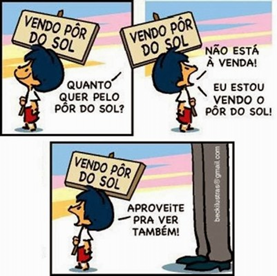
\includegraphics[width=2.88542in,height=2.875in]{./imgSAEB_7_POR/media/image4.png}

\fonte{Armandinho. Disponível em: https://tirasarmandinho.tumblr.com/.
Acesso em: 21 mai. 2023.}
\end{quote}

\num{1} Na tirinha acima pode-se perceber que o humor está presente. Qual  palavra está sendo usada para produzir esse efeito?

\linhas{1}
\coment{A forma verbal `vendo'' é utilizada para obter o efeito do 
humor na tira.} 

\num{2} Por que o uso dessa palavra produz efeito de humor?

\linhas{2}
\coment{No contexto da tirinha, a palavra ``vendo'' pode ter assumir
sentidos diferentes, que causam o efeito de humor.}

\num{3} Quais as possíveis interpretações da palavra usada para produzir
efeito de humor na tirinha?

\linhas{6}
\coment{A forma verbal ``vendo'' é entendida pelo adulto como primeira 
pessoa do singular do presente do indicativo do verbo \textit{vender}, 
isto é: para ele, Armandinho \textit{está vendendo} o pôr do sol. 
Armandinho, por sua vez, quer dizer, por meio da placa, que está 
\textit{observando} o pôr do sol; neste sentido, ``vendo'' é gerúndio do
verbo \textit{ver}.} 

\num{4} Em qual sentido a forma verbal ``vendo'' está sendo usada pelo
personagem Armandinho?

\linhas{4}
\coment{Armandinho quer dizer, por meio da placa, que está 
\textit{observando} o pôr do sol; neste sentido, ``vendo'' é gerúndio do
verbo \textit{ver}.} 

\num{5} Em qual sentido está sendo compreendida a forma verbal ``vendo''
pelo adulto?

\linhas{4}
\coment{A forma verbal ``vendo'' é entendida pelo adulto como primeira 
pessoa do singular do presente do indicativo do verbo \textit{vender}, 
isto é: para ele, Armandinho \textit{está vendendo} o pôr do sol.}

\num{6} Em qual quadrinho a questão das diferentes interpretações da 
forma verbal se esclarece?

\linhas{1}
\coment{As diferentes interpretações da forma verbal se esclarecem 
no último quadrinho.}

Analise a charge abaixo e responda às questões de 7 a 10. 

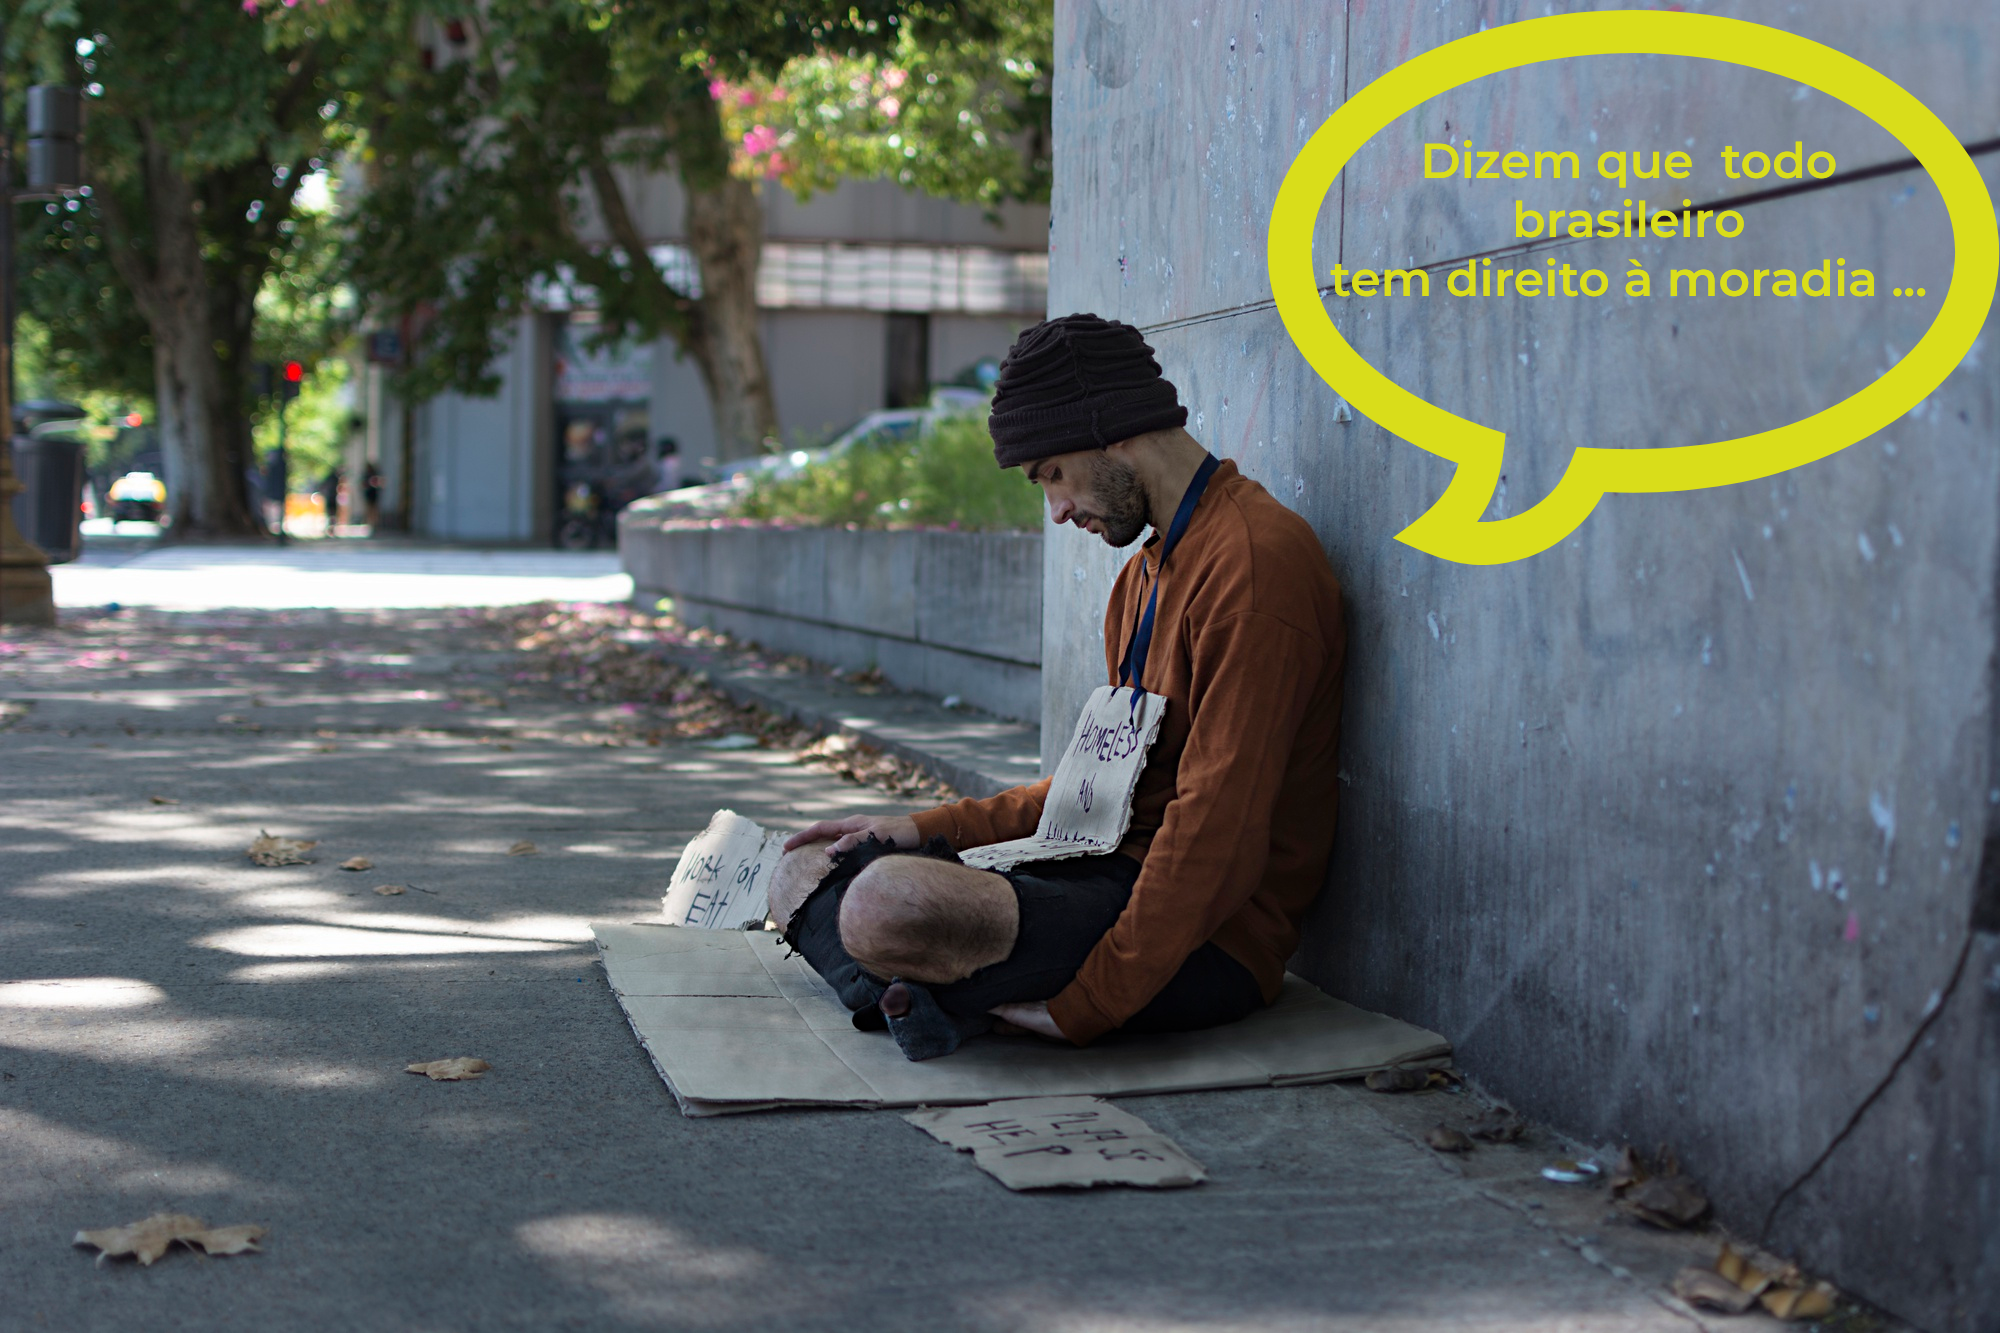
\includegraphics[width=5in,height=3.65625in]{./imgSAEB_7_POR/media/image5.png}

\fonte{Arionauro. Disponível em: http://www.arionaurocartuns.com.br/search/label/charges?updated-max=2022-12-15T14:30:00-08:00\&max-results=20\&start=40\&by-date=false. Acesso em: 21 mai. 2023.}

\num{7} Considerando a imagem e o contexto em que se insere, é possível
inferir qual é o livro que o homem está lendo na tirinha. Que livro é
esse?

\linhas{1}
\coment{É possível inferir que o livro que o homem está lendo é a 
Constituição Federal de 1988.}

\num{8} Qual a função deste documento e o que ele pretende garantir?

\linhas{5}
\coment{A Constitução Federal trata das questões mais importantes 
para a manutenção da democracia e pretende esclarecer os direitos 
e deveres de todos os âmbitos da sociedade.}

\num{9} Qual o efeito de sentido obtido por meio da charge? 

\linhas{5}
\coment{O efeito de sentido obtido por meio da charge é a ironia.}

\num{10} De que forma a imagem se articula com o texto para produzir
o efeito de sentido

\linhas{5}
\coment{ Na charge, uma pessoa em situação de rua lê um dos direitos 
fundamentais garantidos pela Constituição Federal de 1988: o direito à
 moradia. A \textit{declaração} desse direito é rigorosamente oposta à 
\textit{situação concreta} em que se encontra o morador. Essa oposição
compõem a ironia, que consiste em dizer o inverso do que se quer afirmar.
Evidentemente, o autor pretende evidenciar o contraste entre discurso e
prática, entre a afirmação dos direitos na Constituição de 1988 e a 
desigualdade social.} 

\colorsec{Treino}

\num{1} Leia o trecho abaixo para responder à questão. 

\begin{quote}

Há meio século, os escravos fugiam com frequência. Eram muitos, e nem todos
gostavam da escravidão. Sucedia ocasionalmente apanharem pancada, e nem todos
gostavam de apanhar pancada. Grande parte era apenas repreendida; havia alguém de
casa que servia de padrinho, e o mesmo dono não era mau; além disso, o sentimento da
propriedade moderava a ação, porque dinheiro também dói. A fuga repetia-se,
entretanto. Casos houve, ainda que raros, em que o escravo de contrabando, apenas
comprado no Valongo, deitava a correr, sem conhecer as ruas da cidade.

\end{quote}

\finte{Machado de Assis. Pai contra Mãe. Disponível em: 
http://www.dominiopublico.gov.br/download/texto/bv000245.pdf.
Acesso em: 22 mai. 2023.}

No fragmento do conto ``Pai contra Mãe'', o narrador de Machado de Assis faz a crítica
à escravidão brasileira por meio de:

\begin{escolha}

  \item repetições que resultam em ironia.
  
  \item relato objetivo da realidade.
  
  \item observações nostálgicas. 
  
  \item valorização dos escravizados. 

\end{escolha}

\coment{SAEB: Inferir, em textos multissemiótico, efeitos de humor, ironia e/ou
crítica.

a) Correta. Nos primeiros períodos do parágrafo, a repetição de 
``nem todos gostavam'', seguida de expressões que se referem à brutalidade
com que os escravizados eram tratados, dirige o olhar do leitor à violência
por eles vivida, naturalizando a linguagem da brutalidade e resultando na 
ironia, por meio da qual Machado de Assis critica a escravidão.
b) Incorreta. Embora haja passagens descritivas da realidade no fragmento, 
a crítica de Machado de Assis só se constitui por meio das ironias no conjunto. 
c) Incorreta. A nostalgia observável em alguns trechos não é suficiente para
estabelecer a crítica, que só terá lugar por meio da naturalização da linguagem
violenta da escravidão. 
d) Incorreta. Não se observa, no texto, a valorização dos escravizados. Evidentemente
Machado de Assis reproduz, no conjunto, a linguagem que os depreciava, evidenciando
a naturalização da brutalidade contra eles.}


\num{2} Observe a imagem abaixo para responder à questão. 

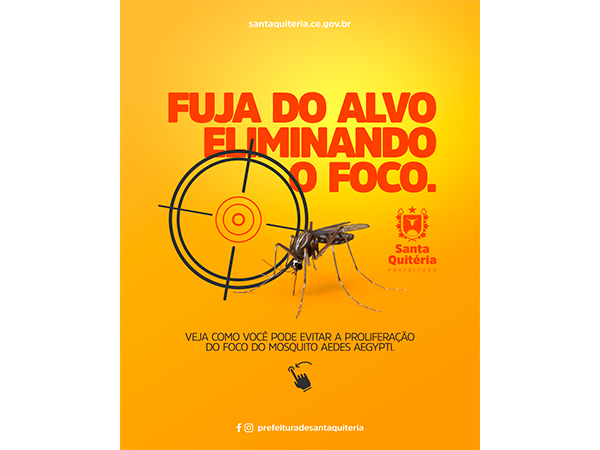
\includegraphics[width=5.90551in,height=4.43056in]{./imgSAEB_7_POR/media/image6.png}

\fonte{Prefeitura de Santa Quitéria. Dicas de como evitar a proliferação 
do foco do mosquito Aedes Aegypti. Disponível em: 
https://www.santaquiteria.ce.gov.br/informa.php?id=1018.
Acesso em: 22 mai. 2023.}

Na imagem acima observa-se uma campanha para evitar a proliferação do
mosquito da dengue. A escolha das palavras e imagens tem como objetivo
sensibilizar a população. Assinale a alternativa que contém as palavras
usadas para a produção de efeito de sentido na campanha. 

\begin{escolha}
  
  \item Proliferação e foco.
  
  \item Veja e evitar.
  
  \item Fuja e elimine.
  
  \item Alvo e foco. 

\end{escolha}

\coment{SAEB: Inferir, em textos multissemiótico, efeitos de humor, ironia e/ou
crítica

BNCC: EF69LP05 -- Inferir e justificar, em textos multissemióticos --
tirinhas, charges, memes, gifs etc. --, o efeito de humor, ironia e/ou
crítica pelo uso ambíguo de palavras, expressões ou imagens ambíguas, de
clichês, de recursos iconográficos, de pontuação etc.

a) Incorreta. A força da campanha é dada pelo jogo entre as palavras
``alvo'' e ``foco''.
b)Incorreta. A força da campanha é dada pelo jogo entre as palavras
``alvo'' e ``foco''.
c)Incorreta. A força da campanha é dada pelo jogo entre as palavras
``alvo'' e ``foco''.
d) Correta. A força da campanha é dada pelo jogo entre as palavras
``alvo'' e ``foco''. De acordo com o texto, deixar de ser alvo do mosquito da
dengue, é preciso eliminar o foco da doença. Além da sonoridade semelhante (ambas
são paroxítonas de duas sílabas terminadas em vogal ``o''), as duas palavras


\num{3}

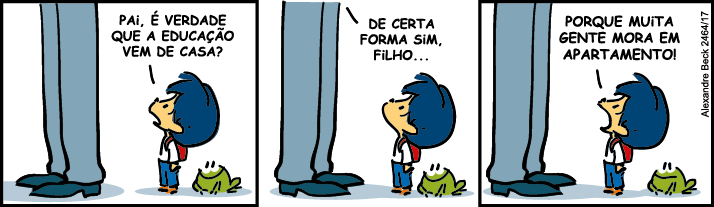
\includegraphics[width=5.90551in,height=1.70833in]{./imgSAEB_7_POR/media/image7.png}

\href{https://tirasarmandinho.tumblr.com/}{\uline{https://tirasarmandinho.tumblr.com/}}
Acesso em 12 de abr 2023.

Leia a tirinha acima e a assinale a alternativa que apresenta o efeito
de sentido produzido:

\begin{escolha}

\item
  a tirinha apresenta ironia sobre a educação com o uso ambíguo da
  palavra casa
\item
  a tirinha apresenta crítica à falta de moradia com o uso da palavra
  casa
\item
  a tirinha apresenta uma crítica às pessoas que moram em casas
\item
  a tirinha questiona o fato de pessoas morarem em apartamentos e não em
  casas
\end{escolha}

Saeb: Inferir, em textos multissemiótico, efeitos de humor, ironia e/ou
crítica

Bncc:(EF69LP05) Inferir e justificar, em textos multissemióticos --
tirinhas, charges, memes, gifs etc. --, o efeito de humor, ironia e/ou
crítica pelo uso ambíguo de palavras, expressões ou imagens ambíguas, de
clichês, de recursos iconográficos, de pontuação etc.

\begin{enumerate}
\def\labelenumi{\arabic{enumi}.}
\tightlist
\item
  Correta. A palavra casa é utilizada em dois sentidos diferentes
\end{enumerate}

b)Incorreta. a tirinha não critica a falta de moradia e sim apresenta
uma ironia sobre a educação das pessoas

\begin{enumerate}
\def\labelenumi{\arabic{enumi}.}
\tightlist
\item
  Incorreta a tirinha não apresenta esse tipo de crítica
\end{enumerate}

d)Incorreta. a tirinha não faz alusão a esse fato

Nível difícil


\chapter{Parcialidade nos textos jornalísticos}
\markboth{Módulo 7}{}

\colorsec{Habilidades do SAEB}

\begin{itemize}

  \item Analisar marcas de parcialidade em textos jornalísticos.

  \item Avaliar diferentes graus de parcialidade em textos jornalísticos.

  \item Avaliar a fidedignidade de informações sobre um mesmo fato divulgado 
  em diferentes veículos e mídias.

\end{itemize}

\colorsec{Habilidades da BNCC}

\begin{itemize}

  \item EF07LP02, EF67LP03, EF67LP04.

\end{itemize}

\conteudo{A função ideal do jornalismo é informar de forma imparcial e objetiva
fatos e notícias para oferecer informações e ferramentas para a
formação de opinião. No entanto, nem sempre é possível separar os fatos
das opiniões, pois todo texto, em alguma medida, é produzido a partir
das perspectivas pessoais do autor ou do veículo de comunicação que o
divulga. Por isso, é importante que os leitores aprendam a analisar
marcas de parcialidade em textos jornalísticos, a fim de avaliar o grau
de confiabilidade das informações que estão recebendo.

Uma das formas de identificar as marcas de parcialidade em textos
jornalísticos é perceber o conjunto de valores expressos pelo uso de
adjetivos, advérbios e na forma como são construídos os argumentos nos
textos de divulgação de notícias e acontecimentos. Também a escolha de
fontes e a seleção editorial dos assuntos e temas a serem tratados podem
indicar interesses e, portanto, certo grau de parcialidade. A escolha
dos pontos de vista expressos em uma notícia ou reportagem revela muito
sobre as intenções do autor ou do veículo que divulga o texto. Sendo
assim, comparar fontes e analisar de forma atenta os contextos em que as
informações são divulgadas em cada veículo de informação pode ser uma
forma eficaz de avaliar a confiabilidade e fidedignidade de determinada
notícia ou reportagem, porque a linha editorial e a relação dos
veículos de comunicação com empresas e grupos políticos ou econômicos
podem revelar possíveis interesses e pontos de vista. Portanto, aprender
a avaliar tais marcas de parcialidade e comparar diferentes formas de
divulgação de notícias em diversos veículos e texto é uma habilidade
importante para que o leitor possa formar uma opinião de forma reflexiva
e autônoma.}

\coment{Professor(a), faça um exercício de reflexão com os estudantes,
questionando como percebem os traços e interesses presentes em algumas
manchetes, e chamadas. Chame a atenção para veículos sensacionalistas,
para determinados temas e assuntos abordados e veiculados com a intenção
de gerar polêmicas, discussões ou busca de soluções. Converse com os
estudantes sobre os diversos tipos de textos jornalísticos e estimule-os
a refletir sobre como percebem as marcas de parcialidade. Instrua-os a
pesquisar e questionar os veículos de comunicação trazendo para a
discussão quais podem ser os interesses por trás dos recursos e
elementos multissemióticos presentes nas informações que consomem. Cite
a monetização de determinados conteúdos, explique como é importante
analisar quem são os financiadores e quais as propagandas e empresas
relacionadas aos veículos de informação que conhecem.}

\colorsec{Atividades}

Analise as duas notícias abaixo e responda às questões.

\begin{quote}

\textbf{Texto I}: Cinco desafios para a economia mundial em 2023}

Se 2022 foi um ano difícil para a economia global, 2023 promete ser
ainda pior, com uma recessão a caminho.

Espera-se que 2023 seja o terceiro ano com o pior crescimento econômico
global neste século, atrás de 2009, quando a crise financeira global
causou a Grande Recessão, e 2020, quando os lockdowns da covid-19
virtualmente paralisaram a economia global.

Analistas esperam que as principais economias do mundo, incluindo os
Estados Unidos e o Reino Unido, assim como a zona do euro, entrem em
recessão este ano, já que os bancos centrais continuam aumentando as
taxas de juros para moderar a demanda por bens de consumo e serviços, em
um esforço para conter a inflação. 

\fonte{Ashutosh Pandey. DW. Cinco desafios para a economia mundial em 2023.
Disponível em: https://www.dw.com/pt-br/cinco-desafios-para-a-economia-mundial-em-2023/a-64264182.
Acesso em: 22 mai. 2023. com adaptações.}

\end{quote}

\begin{quote}

\textbf{Texto II}:Por que a inflação mundial deve cair em 2023 (e por que a
notícia não é tão boa)

Provavelmente o pior em termos de inflação já passou.

Pelo menos este é o consenso entre os economistas e as principais
organizações econômicas como o Fundo Monetário Internacional (FMI) ou o
Banco Mundial depois que a maioria dos países do mundo experimentou, em
2022, aumentos de preços não vistos em quatro décadas.

Não há dúvida de que a inflação continuará a pesar no bolso de milhões
de cidadãos em 2023, mas deve registrar uma queda lenta nos próximos 12
meses.

Quando esse período terminar, o FMI espera que a inflação mundial caia
para 4,7\%, pouco menos da metade do nível atual. 

\end{quote}

\fonte{Cristina J. Orgaz. BBC News Brasil. Por que a inflação mundial deve cair em 2023 (e por que a notícia não é tão boa). 
Disponível em: https://www.bbc.com/portuguese/internacional-64145595.
Acesso em: 22 mai. 2023.}

\num{1} Qual é o fato central relatado nas notícias?

\linhas{1}
\coment{O fato central das duas notícias é a crise econômica de 2023.}

\num{2} Quais são as semelhanças entre os fatos noticiados sobre o tema?

\linhas{3}
\coment{As duas notícias tratam da recessão e da influência da queda da
inflação na crise econômica mundial.}

\num{3} Quais são as diferenças entre os fatos noticiados sobre o tema?

\linhas{5}
\coment{No primeiro texto, o autor prevê, em 2023, a continuidade da crise
econômica. O autor segundo sinaliza, por sua vez, uma queda na inflação.} 

\num{4} Em qual das duas notícias a crise mundial é tratada com mais otimismo?
Copie do texto um trecho que justifique sua resposta.

\linhas{3}
\coment{O Texto II é mais otimista, como se verifica no trecho 
``Provavelmente o pior em termos de inflação já passou''.

\num{5} Na tabela abaixo, relacione os títulos numerados à esquerda
com as linhas finas à direita.

  % Please add the following required packages to your document preamble:
% \usepackage[table,xcdraw]{xcolor}
% If you use beamer only pass "xcolor=table" option, i.e. \documentclass[xcolor=table]{beamer}
\begin{table}[]
\begin{tabular}{|ll|lc|}
\hline
\rowcolor[HTML]{CBCEFB} 
\multicolumn{2}{|c|}{\cellcolor[HTML]{CBCEFB}\textbf{Título}} & \multicolumn{2}{c|}{\cellcolor[HTML]{CBCEFB}\textbf{Linha fina}} \\ \hline
\multicolumn{1}{|l|}{(1)} & \cellcolor[HTML]{FFFFFF}Estudiosos alertam para os riscos de doenças cardiovasculares e o sedentarismo & \multicolumn{1}{l|}{(            )} & \cellcolor[HTML]{FFFFFF}\begin{tabular}[c]{@{}c@{}}Análise de hábitos de pacientes com problemas cardiovasculares traz\\ novas informações sobre como prevenir doenças crônicas\end{tabular} \\ \hline
\rowcolor[HTML]{DAE8FC} 
\multicolumn{1}{|l|}{\cellcolor[HTML]{DAE8FC}(2)} & Casos de dengue preocupam secretarias de saúde & \multicolumn{1}{l|}{\cellcolor[HTML]{DAE8FC}(            )} & \begin{tabular}[c]{@{}c@{}}Associação brasileira de pediatria publica estudo sobre os impactos\\ dos jogos e redes sociais na vida de adolescentes\end{tabular} \\ \hline
\multicolumn{1}{|l|}{(3)} & \cellcolor[HTML]{FFFFFF}O perigo está em casa: Pediatras alertam sobre o uso excessivo de telas por crianças e adolescentes & \multicolumn{1}{l|}{(            )} & \cellcolor[HTML]{FFFFFF}\begin{tabular}[c]{@{}c@{}}Ministério da saúde lança cartilha para informar a população sobre\\ as formas de contágio da doença\end{tabular} \\ \hline
\rowcolor[HTML]{DAE8FC} 
\multicolumn{1}{|l|}{\cellcolor[HTML]{DAE8FC}(4)} & Covid-19: Informar para proteger & \multicolumn{1}{l|}{\cellcolor[HTML]{DAE8FC}(            )} & \begin{tabular}[c]{@{}c@{}}Alerta foi dado às secretarias de saúde de todo país, especialmente\\ nas regiões em que se inicia o período de chuvas\end{tabular} \\ \hline
\end{tabular}
\end{table}

\coment{1, 3, 4, 2}

\num{6} Sobre a parcialidade dos textos jornalísticos, assinale V para as
afirmações verdadeiras e F para as afirmações falsas na tabela abaixo.

% Please add the following required packages to your document preamble:
% \usepackage[table,xcdraw]{xcolor}
% If you use beamer only pass "xcolor=table" option, i.e. \documentclass[xcolor=table]{beamer}
\begin{table}[]
\begin{tabular}{|l|l|}
\hline
\rowcolor[HTML]{9698ED} 
\multicolumn{1}{|c|}{\cellcolor[HTML]{9698ED}\textbf{\begin{tabular}[c]{@{}c@{}}Verdadeiro (V) \\ ou \\ Falso (F)\end{tabular}}} & \multicolumn{1}{c|}{\cellcolor[HTML]{9698ED}\textbf{Afirmação}} \\ \hline
 & \begin{tabular}[c]{@{}l@{}}A imparcialidade no jornalismo é importante pois promove a formação\\ de opinião a partir dos fatos apresentados na reportagem\end{tabular} \\ \hline
\rowcolor[HTML]{ECF4FF} 
 & \begin{tabular}[c]{@{}l@{}}O princípio da imparcialidade no jornalismo significa que o\\ jornalista não deve apresentar os diferentes pontos de vista e deixar\\ que o público forme sua própria opinião\end{tabular} \\ \hline
 & \begin{tabular}[c]{@{}l@{}}A imparcialidade no jornalismo pode levar a erros de interpretação e\\ compreensão dos fatos por parte do público, prejudicando a credibilidade\\ da reportagem do jornalista\end{tabular} \\ \hline
\rowcolor[HTML]{ECF4FF} 
 & \begin{tabular}[c]{@{}l@{}}A falta de apresentação de fontes e dados confiáveis pode ser uma\\ característica de parcialidade por parte do jornalista ou do veículo de\\ comunicação colocando em dúvida a credibilidade das notícias veiculadas\end{tabular} \\ \hline
\end{tabular}
\end{table}

\coment{V, F, V, V}

\num{7} Leia os exemplos abaixo e sublinhe as marcas de parcialidade:

\begin{escolha}

  \item Polícia age com violência contra manifestantes pacíficos.

  \item Deputado faz discurso inflamado em defesa dos direitos dos
trabalhadores.

  \item Falas preconceituosas de senadores exibem a impunidade da classe
política no Brasil.

\end{escolha}

\coment{a) Polícia age com \uline{violência} contra manifestantes
\uline{pacíficos}.

b) Deputado faz discurso \uline{inflamado} em defesa dos direitos dos
trabalhadores.

c) Falas \uline{preconceituosas} de senadores exibem a
\uline{impunidade} da classe política no Brasil.}

\num{8} Quais aspectos devem ser levados em conta para questionar a
parcialidade ou imparcialidade de uma notícia

\linhas{8}
\coment{Os aspectos que devem ser levados em conta são: a exposição de
mais de um ponto de vista sobre o mesmo tema, a citação de dados e 
pesquisas de fontes confiáveis e o uso ou não de adjetivos que qualifiquem
os fatos apresentados. É importante também a checagem da veracidade dos 
dados apresentados e o questionamento sobre os contextos em que ocorrem os
fatos e se há interesses políticos ou econômicos por parte do veículo de
comunicação que divulga a notícia.}

\num{9} Analise as duas afirmações a seguir e responda qual das duas apresenta
maior grau de parcialidade. Justifique sua resposta

\begin{itemize}
 
 \item Policiamento nas cidades não gera mais segurança, é o que afirmam
especialistas

  \item Policiamento nas cidades é a principal medida de segurança anunciada pela prefeitura.

\end{itemize}

\linhas{6}
\coment{A primeira afirmação apresenta maior grau de parcialidade, pois
apresenta uma afirmação categórica amparada em afirmação de especialistas. 
A segunda é uma sentença menos parcial, embora contenha o adjetivo ``principal'' para referir-se ao fato noticiado.}

\num{10} De que forma a apresentação de imagens, gráficos e tabelas auxilia 
na formação de opinião de leitores?
\linhas{5}
  
e  a trazer mais credibilidade à notícia, pois podem ser interpretados, 
questionados e verificados.}

\colorsec{Treino}

\num{1} Sabendo da importância de aprender a analisar traços de parcialidade em
textos jornalísticos, assinale a alternativa que contém um recurso por meio
do qual o texto jornalístico tende a ser mais parcial.

\begin{escolha}

  \item Entrevistas com especialistas no assunto abordado.
  \item Diferentes pontos de vista sobre o mesmo assunto.
  \item Adjetivos valorativos para descrever pessoas ou eventos.
  \item Fatos e fontes citadas rigorosamente. 

\end{escolha}

\coment{SAEB: Analisar marcas de parcialidade em textos jornalísticos.

a) Incorreta. Entrevistas com especialistas pretendem obter o efeito da 
imparcialidade.
b) Incorreta. A apresentação de diferentes pontos de vista pretende obter
o efeito da imparcialidade. 
c) Correta. A presença de adjetivos valorativos é marca de parcialidade.
d) Incorreta. A presença de fontes e fatos pretende obter
o efeito da imparcialidade.}

\num{2} Leia o trecho abaixo e o gráfico que segue para responder à questão.

\begin{quote}

Não estamos no caminho certo para atingir as metas de mudança
climática. Se somarmos todas as promessas para reduzir emissões de gases
que provocam efeito estufa pelos países que assinaram o Acordo de Paris,
o mundo ainda esquentaria em mais de 3°C até o fim deste século.

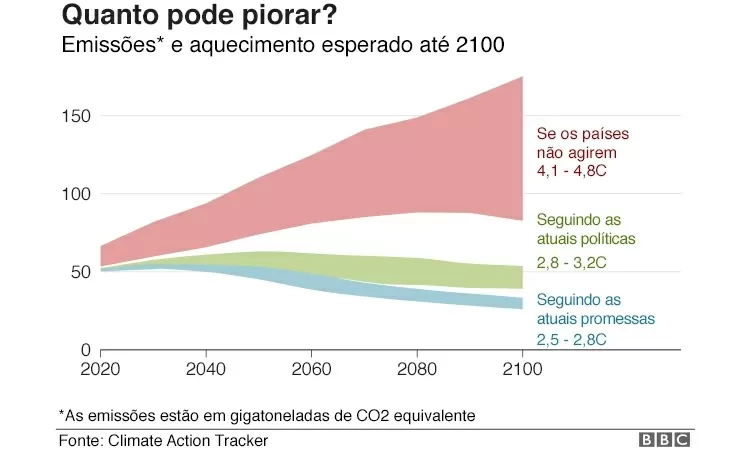
\includegraphics[width=5.90551in,height=3.56944in]{./imgSAEB_7_POR/media/image8.png}

\fonte{BBC News Brasil. Aquecimento global: 7 gráficos que mostram em que ponto estamos. Disponível em: https://www.bbc.com/portuguese/geral-46424720. 
Acesso em: 22 mai. 2023.}

Assinale a alternativa que contém o principal recurso para obter o efeito da 
confiabilidade da notícia:

\begin{escolha}

  \item a opinião do jornalista.
  
  \item a oposição ao Acordo de Paris.
  
  \item o uso de gráficos de pesquisas.
  
  \item o uso de expressões sensibilizadoras.

\end{escolha}

\ciment{SAEB:Avaliar diferentes graus de parcialidade em textos jornalísticos.

BNCC: EF67LP04 -- Distinguir, em segmentos descontínuos de textos,
fato da opinião enunciada em relação a esse mesmo fato.

a) Incorreta. A opinião do jornalista não é um recurso de imparcialidade.
b)Incorreta. O autor não se opõe ao Acordo de Paris, citado como referência às metas
para reversão da situação climática.
c)Correta. O uso de gráficos e recursos similares trazem maior clareza, possibilitando
ao leitor formar suas próprias opiniões
d)Incorreta. O uso de expressões que pretendem sensibilizar o leitor são recursos de
persuasão importantes, mas não conferem imparcialidade ao texto.}

\num{3}

\begin{quote}

\textbf{Após três anos sem reajuste, tarifa de ônibus é corrigida abaixo da
inflação do período}

A partir de 1° de janeiro de 2023, o transporte coletivo urbano de
Joinville passará a operar com os valores de R\$5,25 para a tarifa
antecipada e R\$5,50 para a tarifa embarcada (modalidade utilizada por
apenas 5\% dos passageiros). O reajuste representa aproximadamente
metade do percentual de inflação dos últimos três anos, período no qual
a tarifa não foi corrigida.

\end{quote}

\fonte{Prefeitura de Joinville. Após três anos sem reajuste, tarifa de ônibus é 
corrigida abaixo da inflação do período. Disponível em: https://www.joinville.sc.gov.br/noticias/apos-tres-anos-sem-reajuste-tarifa-de-onibus-e-corrigida-abaixo-da-inflacao-do-periodo/
Acesso em: 22 mai. 2023.}

A matéria apresenta grau de parcialidade, pois apresenta:

\begin{escolha}
  
  \item justificativa para o aumento desde o título.
  
  \item informações precisas sobre a data do ocorrido
  
  \item informações sobre os valores da passagem
  
  \item dados sobre os usuários do transporte público na cidade

\end{escolha}

\coment{SAEB:Analisar marcas de parcialidade em textos jornalísticos.

BNCC: EF67LP04 -- Distinguir, em segmentos descontínuos de textos,
fato da opinião enunciada em relação a esse mesmo fato.

a)Correta. Já no título a notícia apresenta argumentos que levam a crer na
necessidade de reajuste.
b) Incorreta. Essas informações não representam a opinião do veículo e 
podem ser considerados recursos para atribuir veracidade à notícia.
c) Incorreta. Essas informações não representam a opinião do veículo e 
podem ser considerados recursos para atribuir veracidade à notícia.
d) Incorreta. Essas informações não representam a opinião do veículo e 
podem ser considerados recursos para atribuir veracidade à notícia.}

\chapter{Recursos de modalização e argumentação}
\markboth{Módulo 8}{}

\colorsec{Habilidades do SAEB}

\begin{itemize}

  \item Identificar os recursos de modalização em textos diversos.

  \item Analisar os efeitos de sentido dos tempos, modos e/ou vozes 
verbais com base no gênero textual e na intenção comunicativa.

  \item Analisar os efeitos de sentido produzidos pelo uso de modalizadores em textos diversos.

\end{itemize}

\colorsec{Habilidades da BNCC}

\begin{itemize}

  \item EF69LP04, EF69LP28, EF07LP14.

\end{itemize}

\conteudo{A capacidade de identificar e compreender os recursos de modalização
presentes em diferentes tipos de texto é fundamental para uma
comunicação eficiente e coerente. A modalização envolve o uso de
recursos linguísticos para expressar atitudes e opiniões do emissor em
relação ao conteúdo abordado. Esses recursos podem estar
presentes nas formas de uso de modos e vozes verbais, além de adjetivos e advérbios.

A análise dos efeitos de sentido produzidos pelos recursos de
modalização em diferentes gêneros textuais e intenções comunicativas é
fundamental para identificar as influências destes recursos na percepção
e compreensão do conteúdo pelo receptor.

Os recursos de modalização permitem que o emissor expresse suas
opiniões, transmita suas expectativas, faça indicações, influenciando
assim na percepção dos leitores. Dentre os principais recursos
de modalização, encontram-se os tempos verbais, os modos verbais, as
vozes verbais e os modalizadores, que podem reformar graus de
probabilidade, certeza, necessidade e urgência.

Portanto, compreender e utilizar os recursos de modalização de forma
adequada é essencial para produzir textos claros, coerentes e
persuasivos, adaptando a linguagem ao tipo de público alvo e ao contexto
em que são emitidos. Além disso, a análise crítica desses recursos
permite que o leitor compreenda as intenções do emissor e as influências
que podem estar presentes no conteúdo do texto.}

\coment{Professor(a), estimule os estudantes a lembrarem do uso destes recursos
em exemplos conhecidos e práticos tais como campanhas de conscientização
ou publicitárias. Retome os recursos de modalização presentes em
diversos gêneros textuais já estudados demonstrando as diferenças de
interpretação e sentido possíveis para os usos de tempos e modos
verbais, tais como infinitivo e imperativo, das vozes do texto, dos
discursos diretos e indiretos e do uso de advérbios que qualificam as
ações com advérbios que indicam urgência, condições, sugestões,
obrigatoriedade, etc.}

\colorsec{Atividades}


\includegraphics[width=2.85536in,height=2.85536in]{./imgSAEB_7_POR/media/image9.png}

\href{https://itajuba.mg.gov.br/secretariaspmi/semdes/nao_desvie_o_olhar/}{\uline{https://itajuba.mg.gov.br/secretariaspmi/semdes/nao\_desvie\_o\_olhar/}}.
Acesso em 18 de abr de 2023

\num{1} Retire da imagem acima os elementos modalizadores que produzem o sentido de instrução.

\linhas{1}
\coment{As formas verbais no imperativo produzem o sentido de instrução no texto.}

\num{2} De que forma o uso desses recursos sensibiliza o leitor?

\linhas{3}
\coment{As formas verbais no imperativo apelam para a responsabilidade individual do leitor quanto
à violência contra crianças e adolescentes.}

\num{3} Observe as informações contidas no cartaz e explique qual é a ação
recomendada ao tomar conhecimento de casos de violência contra crianças e adolescentes.

\linhas{2}
\coment{Ligar para o telefone indicado e denunciar a violência contra crianças e adolescentes é 
a ação recomendada.}

\num{4} Relacione as colunas de expressões com seus respectivos efeitos de sentido:

% Please add the following required packages to your document preamble:
% \usepackage[table,xcdraw]{xcolor}
% If you use beamer only pass "xcolor=table" option, i.e. \documentclass[xcolor=table]{beamer}
\begin{table}[]
\begin{tabular}{|cc|cc|}
\hline
\rowcolor[HTML]{FD6864} 
\multicolumn{2}{|c|}{\cellcolor[HTML]{FD6864}\textbf{Efeito de sentido}} & \multicolumn{2}{c|}{\cellcolor[HTML]{FD6864}\textbf{Expressão}} \\ \hline
\multicolumn{1}{|c|}{\textbf{I}} & Obrigação & \multicolumn{1}{c|}{} & felizmente \\ \hline
\rowcolor[HTML]{FFCCC9} 
\multicolumn{1}{|c|}{\cellcolor[HTML]{FFCCC9}\textbf{II}} & Apreciação & \multicolumn{1}{c|}{\cellcolor[HTML]{FFCCC9}} & é dever de todos \\ \hline
\multicolumn{1}{|c|}{\textbf{III}} & Possibilidade & \multicolumn{1}{c|}{} & é impossível \\ \hline
\rowcolor[HTML]{FFCCC9} 
\multicolumn{1}{|c|}{\cellcolor[HTML]{FFCCC9}\textbf{IV}} & Certeza & \multicolumn{1}{c|}{\cellcolor[HTML]{FFCCC9}} & provavelmente \\ \hline
\end{tabular}
\end{table}

\coment{II, I, IV, III}

Leia a afirmação abaixo e responda à questão.

\begin{quote}

\textbf{Certamente}, com a implementação dos projetos de mobilidade
urbana, as pessoas passarão a ter mais qualidade de vida e mais
liberdade para explorar e ocupar a cidade.

\end{quote}

\num{5} Qual sentido a palavra destacada pretende expressar?

\linhas{2}
\coment{A palavra destacada pretende expressar certeza sobre as consequências da melhoria da
mobilidade urbana.}

Observe a campanha a seguir e responda:


\includegraphics[width=5.90551in,height=1.47222in]{./imgSAEB_7_POR/media/image10.png}

\fonte{Agência de Transporte do Estado de São Paulo. #FocaNaVida. Disponível em:
http://www.artesp.sp.gov.br/Style\%20Library/extranet/campanha-interna.aspx?id=1
Acesso em: 22 mai. 2023.}

\num{6} Qual a ideia transmitida pela conjunção ``se'' na frase, 
``Nesse carnaval se beber, não dirija''?

\linhas{2}
\coment{A conjunção ``se'', na frase analisada, é condicional, ou seja, é por meio dela que 
se propõe a condição expressa na frase: caso o leitor tenha bebido, não deve dirigit.} 

\num{7} Ainda sobre a campanha acima, assinale verdadeiro ou falso na tabela para as afirmações a seguir.

% Please add the following required packages to your document preamble:
% \usepackage[table,xcdraw]{xcolor}
% If you use beamer only pass "xcolor=table" option, i.e. \documentclass[xcolor=table]{beamer}
\begin{table}[]
\begin{tabular}{|l|c|}
\hline
\rowcolor[HTML]{9AFF99} 
\multicolumn{1}{|c|}{\cellcolor[HTML]{9AFF99}\textbf{\begin{tabular}[c]{@{}c@{}}Verdadeiro (V)\\ ou\\ Falso (F)\end{tabular}}} & \textbf{Afirmação} \\ \hline
 & a campanha sugere que não se deve dirigir após beber \\ \hline
\rowcolor[HTML]{FFFFC7} 
 & a campanha sugere que as pessoas não devem beber durante o carnaval \\ \hline
 & a campanha orienta os foliões a não dirigir no carnaval \\ \hline
\rowcolor[HTML]{FFFFC7} 
 & a campanha pretende alertar sobre a violência no trânsito \\ \hline
\end{tabular}
\end{table}

\coment {V, F, F, F}

\num{8} Leia os enunciados e enumere as proposições na tabela.

% Please add the following required packages to your document preamble:
% \usepackage[table,xcdraw]{xcolor}
% If you use beamer only pass "xcolor=table" option, i.e. \documentclass[xcolor=table]{beamer}
\begin{table}[]
\begin{tabular}{|c|c|c|c|}
\hline
\rowcolor[HTML]{ECF4FF} 
 & Enunciado &  & Efeito \\ \hline
1 & É necessária a presença de um acompanhante &  & Expressa proibição \\ \hline
2 & É proibida a entrada de acompanhante &  & Expressa obrigatoriedade \\ \hline
3 & É permitida a entrada de um acompanhante &  & Expressa permissão \\ \hline
\end{tabular}
\end{table}

\coment{2, 1, 3}

%Leia tirinha abaixo para responder à questão.

%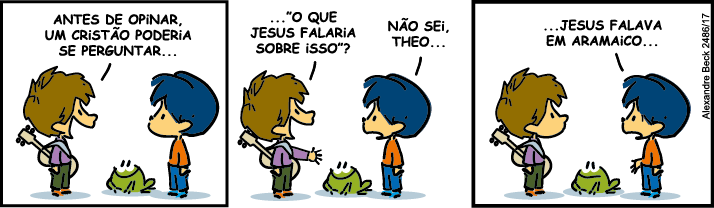
\includegraphics[width=5.90551in,height=1.72222in]{./imgSAEB_7_POR/media/image11.png}

%\href{https://tirasarmandinho.tumblr.com/}{\uline{https://tirasarmandinho.tumblr.com/}}
%Acesso em 19 de Abr de 2023

%\num{9}
%Qual é a confusão comunicativa presente na tirinha?
%
%
%A confusão se dá pois os personagens entendem o verbo falar em sentidos diferentes

%\num{10} Qual o sentido do verbo falar no segundo quadrinho? Escreva um sinônimo.

%O verbo falar no segundo quadrinho se refere a opinião, e poderia ser
%substituído por dizer ou pensar. Pensaria, diria.

\colorsec{Treino}

\num{1} Leia o texto abaixo para responder à questão.

\begin{quote}

Antes da pandemia causada pelo novo coronavírus, era quase impensável
ver grande parte da população usando máscaras de proteção na rua.
Contudo a situação mudou, principalmente após o governo do estado tornar
seu uso obrigatório. Mesmo assim, ainda há dúvidas de parte da população
quanto à necessidade e ao benefício do seu uso.

\end{quote}

\fonte{Secretaria de Estado de Saúde de Minas Gerais. Notas de Recomendação: Covid 19.
Disponível em: https://coronavirus.saude.mg.gov.br/blog/101-mascaras-e-covid-19.
Acesso em: 22 mai. 2023.}

No contexto em que se insere, a expressão ``mesmo assim'' expressa oposição entre:


\begin{escolha}

  \item o período anterior e o posterior à pandemia do coronavírus.

  \item a alta adesão da população ao uso de máscaras e a obrigatoriedade de usá-las.

  \item a obrigatoriedade do uso de máscaras e a atitude da população quanto a essa medida.

  \item grande parte da população utilizando máscaras de proteção e a minoria em dúvida.

\end{escolha}

\coment{SAEB: Analisar os efeitos de sentido produzidos pelo uso de modalizadores em textos diversos.

BNCC: EF07LP14 -- Identificar, em textos, os efeitos de sentido do
uso de estratégias de modalização e argumentatividade.

a) Incorreta. No trecho em que se insere, a expressão indicada opõe a afirmação anterior, sobre
a obrigatoriedade do uso de máscaras decretada pelo governo, e a posterior, ``ainda há dúvidas 
de parte da população quanto à necessidade e ao benefício do seu uso''. 
b) Incorreta. No trecho em que se insere, a expressão indicada opõe a afirmação anterior, sobre
a obrigatoriedade do uso de máscaras decretada pelo governo, e a posterior, ``ainda há dúvidas 
de parte da população quanto à necessidade e ao benefício do seu uso''.
c) Correta. No trecho em que se insere, a expressão indicada opõe a afirmação anterior, sobre
a obrigatoriedade do uso de máscaras decretada pelo governo, e a posterior, ``ainda há dúvidas 
de parte da população quanto à necessidade e ao benefício do seu uso''.
c)Incorreta. No trecho em que se insere, a expressão indicada opõe a afirmação anterior, sobre
a obrigatoriedade do uso de máscaras decretada pelo governo, e a posterior, ``ainda há dúvidas 
de parte da população quanto à necessidade e ao benefício do seu uso''.}

\num{2} Leia o texto abaixo para responder à questão. 

\begin{quote}

Carlos observava toda aquela pompa ao seu redor. Ele mesmo estava de passagem,
era um turista simples, brasileiro comum, passeando a custo do dinheiro suado, 
guardado todo mês, para conhecer aquela terra estrangeira e faustosa, cheia de 
gente milionária e bem vestida, cheirosa e fútil. Como deve ser triste depender
do luxo para ser feliz! --- pensava ele.     

\end{quote}

\fonte{Rogério Duarte. Viagens pela terra dos outros. Saíra Editorial. no prelo.}

Na frase ``Como \textbf{deve} ser triste depender do luxo para ser feliz!'', 
a forma verbal destacada expressa:

\begin{escolha}
  
  \item Obrigação
  
  \item Conselho
  
  \item Causa
  
  \item Possibilidade

\end{escolha}

\coment{SAEB:Analisar os efeitos de sentido dos tempos, modos e/ou vozes verbais
com base no gênero textual e na intenção comunicativa.

a) Incorreta. A forma verbal ``deve'', no contexto em que se insere, expressa possibilidade.
b) Incorreta. A forma verbal ``deve'', no contexto em que se insere, expressa possibilidade.
c) Incorreta. A forma verbal ``deve'', no contexto em que se insere, expressa possibilidade.
d) Correta. A forma verbal ``deve'', no contexto em que se insere, expressa possibilidade.}

\num{3}

Analise o cartaz abaixo:


\includegraphics[width=5.90551in,height=4.29167in]{./imgSAEB_7_POR/media/image13.png}

\fonte{Ministério da Integração e do Desenvolvimento Regional. Consumo consciente da água 
é base para um futuro sustentável. Disponível em: https://www.gov.br/dnocs/pt-br/assuntos/noticias/consumo-consciente-da-agua-e-base-para-um-futuro-sustentavel.
Acesso em: 22 mai. 2023.}

O uso do gerúndio na campanha acima expressa:

\begin{escolha}

  \item ação contínua.
  \item ordem a ser acatada.
  \item sugestão a ser considerada.
  \item condição.

\end{escolha}

\coment{SAEB: Analisar os efeitos de sentido dos tempos, modos e/ou vozes
verbais com base no gênero textual e na intenção comunicativa.

BNCC: EF69LP04 -- Identificar e analisar os efeitos de sentido
que fortalecem a persuasão nos textos publicitários, relacionando as
estratégias de persuasão e apelo ao consumo com os recursos
linguístico-discursivos utilizados, como imagens, tempo verbal, jogos de
palavras, figuras de linguagem etc., com vistas a fomentar práticas de
consumo conscientes.

a) Incorreta. No contexto em que se insere, a forma verbal no gerúndio tem valor condicional: 
``Água: se soubermos usar, não vai faltar''. 
b) Incorreta. No contexto em que se insere, a forma verbal no gerúndio tem valor condicional: 
``Água: se soubermos usar, não vai faltar''. 
c) Incorreta. No contexto em que se insere, a forma verbal no gerúndio tem valor condicional: 
``Água: se soubermos usar, não vai faltar''.
d) Incorreta. No contexto em que se insere, a forma verbal no gerúndio tem valor condicional: 
``Água: se soubermos usar, não vai faltar''.}  

\chapter{Figuras de linguagem como estratégia argumentativa}
\markboth{Módulo 9}{}

\colorsec{Habilidades do SAEB}

\begin{itemize}
  
  \item Analisar o uso de figuras de linguagem como estratégia argumentativa.

  \item Avaliar a eficácia das estratégias argumentativas em textos de diferentes gêneros.

\end{itemize}

\colorsec{Habilidades da BNCC}

\begin{itemize}

  \item EF69LP17, EF67LP38.

\end{itemize}

\conteudo{A linguagem tem como principal objetivo a comunicação, portanto, é
impossível distinguir a linguagem da interação que ela provoca. Quanto
maior o domínio das ferramentas de linguagem por parte do autor, maior o
nível de interação e conexão será atingido com o leitor. Do outro lado,
quanto maior a capacidade de reconhecimentos das ferramentas e recursos
de expressividade forem conhecidas pelo leitor, melhor será sua
experiência. Existem diversas maneiras de promover maior expressividade
das palavras e com isso, facilitar e potencializar a interação por meio
da comunicação. Dentre esses recursos estão as chamadas figuras de
linguagem. São expressões e formas de interação possíveis à linguagem
que podem trazer maior riqueza de detalhes, maior clareza ou maior
objetividade ao texto, seja ele escrito ou transmitido oralmente.

Cada figura de linguagem tem suas características próprias e pode ser
utilizada de diversas maneiras, de acordo com o objetivo do falante ou
do escritor, com a situação comunicativa e com o interlocutor. As
figuras de linguagem podem fazer alusão ao sentido figurado das palavras
e expressões, tratar com exagero para exacerbar características e
impressões ou contrapor palavras com sentidos antagônicos demonstrando
valores de forma implícita. Por essas características, as figuras de
linguagem são recursos comunicativos de grande utilidade especialmente
para escrita de textos do campo artístico literário como letras de
músicas e poemas. Se apresentam ainda como um recurso de persuasão e
comunicação importante também para os textos do campo jornalístico
midiático.

Sendo assim, a metáfora é uma figura de linguagem utilizada para
estabelecer uma relação de semelhança e comparação entre dois termos
distintos. Um exemplo do uso da metáfora é a expressão "sua vida era um
mar de rosas". Nesse caso, a expressão "mar de rosas" não tem o sentido
literal, mas sim o sentido figurado, pois se refere a algo agradável e
prazeroso e não ao mar em sentido literal.

A metonímia, por sua vez, é a figura de linguagem utilizada quando se
lança mão um termo para se referir a outro, com o qual ele mantém uma
relação de proximidade, continuidade e pertencimento. Ou seja, dizer que
"a cidade se beneficiou com as obras de infraestrutura" é utilizar a
figura de linguagem metonímia, pois, utiliza o termo ' a cidade' para se
referir à população da cidade. A metonímia tem o efeito de tornar a
linguagem mais concisa e precisa, evitando a repetição de termos e
textos muito extensos. É uma forma de dinamizar a comunicação e
potencializar a capacidade comunicativa.

Já a personificação é a figura de linguagem utilizada sempre que se
atribui a animais e objetos, características humanas. A personificação
tem o efeito de tornar a linguagem mais expressiva e poética, pois
humaniza seres e fenômenos produzindo alto grau de identificação do
leitor com a experiência, sensação ou impressão que se pretende
comunicar.

Por fim, a hipérbole é a figura de linguagem que aumenta ou exagera
determinada característica como forma de expressão, pode representar um
exagero para transmitir uma ideia.

\coment{Professor(a) peça aos estudantes que tragam suas impressões, faça um
levantamento dos conhecimentos prévios que já têm. Deixe que tragam
exemplos e forneça mais informações sobre os conceitos, chamando a
atenção para as possibilidades expressivas das figuras de linguagem.
Mostre como o uso das figuras de linguagem podem ampliar os efeitos de
sentido, seja nos textos literários, nos textos jornalísticos, para
efeitos de ironia, humor, etc.}

\colorsec{Atividades}

Que, havendo tanto já que as partes vendo

Onde o dia é comprido e onde breve,

Inclinam seu propósito e perfia

\textbf{A ver os berços onde nasce o dia}.'

Os Lusíadas I-27-8
\href{http://www.dominiopublico.gov.br/download/texto/bv000162.pdf}{\uline{http://www.dominiopublico.gov.br/download/texto/bv000162.pdf}}.
Acesso em 19 de abr de 2023

Analise o trecho destacado e responda:


\num{1}
  Qual a figura de linguagem presente no verso em destaque?

A figura de linguagem presente no verso é a personificação pois atribui
características humanas ao fenômeno natural do nascimento do sol.

\num{2}
  Assinale nas opções abaixo as características da metáfora:
\end{enumerate}

( ) utilizada em textos poéticos

( ) faz comparação entre termos diferentes

( ) Apresenta o termo de comparação

( ) faz uma comparação sem utilizar o termo de comparação

(X) utilizada em textos poéticos

(X) faz comparação entre termos diferentes

( ) Apresenta o termo de comparação

(X) faz uma comparação sem utilizar o termo de comparação

O BURRO E O LEÃO Vinha o burro pelo caminho, na sua ignorância de
sempre. Numa curva, deparou com o leão. --- Saia já da minha frente ---
disse ele, com a presunção dos tolos. O leão olhou bem para o burro e
pensou: "Seria fácil demais dar uma lição a esse infeliz. Não vou sujar
meus dentes e minhas garras com ele." E prosseguiu, muito calmo, sem se
importar com o burro.

Acima, vemos o exemplo de uma fábula. As fábulas, em geral, apresentam
elementos da natureza e animais como personagens principais. Sabendo
disso, retire do texto exemplos de personificação:

O leão olhou bem para o burro e pensou. Dentre outros

\num{3}
  Ao dizer a seguinte frase: Você tem um coração de pedra! Faz-se uso de
  qual figura de linguagem?
\num{4}
  A afirmação `Estou morrendo de medo' sugere o uso de qual figura de
  linguagem?
\num{5}
  As estrelas são os olhos dos deuses, representa qual figura de
  linguagem?
\num{6}
  Associe as frases com a figura de linguagem correspondente:

\num{7}
  Sobre a hiperbole, assinale V para as afirmações verdadeiras e F para
  as falsas:
\end{enumerate}

\begin{quote}
( ) Faz uma comparação entre palavras distintas

( ) pretende exagerar o sentido de uma palavra

( ) expressa ênfase em uma sensação

( ) atribui características humanas a objetos

(F) Faz uma comparação entre palavras distintas

(V) pretende exagerar o sentido de uma palavra

(V) expressa ênfase em uma sensação

( F) atribui características humanas a objetos

Na cordilheira que fica em cima do vale de Yyucay, em Cusco,

pode-se ouvir todos os sons. O vento sopra com sua bocarra;

a manhã, obrigada a se levantar sempre antes dos outros,

boceja morta de sono; os pássaros, seus eternos namorados,

acordam cantando ao ouvi-la se espreguiçar.

http://www.dominiopublico.gov.br/download/texto/me001614.pdf
\end{quote}

\num{8}
  Quais as figuras de linguagem presentes no trecho acima:

Hipérbole, personificação

\num{9}
  Copie do texto um exemplo de hipérbole:

boceja morta de sono

\num{10}
  Copie do texto um exemplo de personificação
\end{enumerate}

O vento sopra com sua bocarra, os pássaros, seus eternos namorados,

acordam cantando ao ouvi-la se espreguiçar.

\colorsec{Treino}

\num{1}

``Brasil reforça postura de neutralidade e ganha espaço na geopolítica
mundial''

O trecho acima apresenta a figura de linguagem metonímia pois:

\begin{enumerate}

\item
  Personifica o país
\item
  compara o Brasil com outros países
\item
  Exagera ao qualificar o Brasil como um país neutro
\item
  Usa o termo Brasil para se referir ao governo do país
\end{enumerate}

Saeb:Avaliar a eficácia das estratégias argumentativas em textos de
diferentes

gêneros.

a)Incorreta. A personificação não é característica da metonímia

b)Incorreta. O texto não faz comparação com outros países

c)Incorreta. O texto não faz alusão isso nem utiliza hipérbole

d)Correta. Nesta alternativa temos a definição de metonímia

Nível Médio

\num{2}

Ao voltar para casa, \textbf{não se cansava de elogiar} a

desconhecida do baile. Nos dias que se seguiram, procurou-a

por toda a fazenda e pelos povoados vizinhos, mas não

conseguiu encontrá-la. E ficou mais triste ainda.

O trecho destacado apresenta a figura de linguagem:

\begin{enumerate}

\item
  metáfora
\item
  hipérbole
\item
  metonímia
\item
  personificação
\end{enumerate}

Saeb: Avaliar a eficácia das estratégias argumentativas em textos de
diferentes

gêneros.

\begin{enumerate}
\def\labelenumi{\arabic{enumi}.}
\tightlist
\item
  Incorreta. O trecho não faz comparação
\end{enumerate}

b)Correta. O trecho exagera o termo para expressar o quanto o rapaz
falava da moça

\begin{enumerate}
\def\labelenumi{\arabic{enumi}.}
\item
  Incorreta. O trecho não utiliza um termo para significar outro termo
  referente
\item
  Incorreta. O trecho não atribui características humanas a objetos
  inanimados ou fenômenos naturais.
\end{enumerate}

Nível Difícil

\num{3}

Leia a tirinha abaixo:

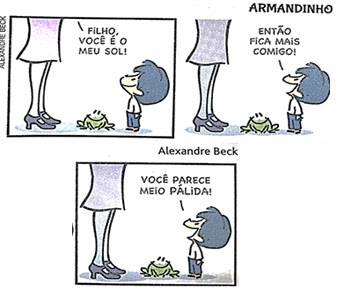
\includegraphics[width=3.51042in,height=3.02083in]{./imgSAEB_7_POR/media/image14.png}

\href{https://tirasarmandinho.tumblr.com/}{\uline{https://tirasarmandinho.tumblr.com/}}.
Acesso em 20 de Abr de 2023.

A mãe de Armandinho expressa seu amor pelo filho fazendo uso de:

\begin{enumerate}

\item
  Hipérbole
\item
  Metáfora
\item
  Personificação
\item
  Metonímia
\end{enumerate}

Saeb: Analisar o uso de figuras de linguagem como estratégia
argumentativa.

a)Incorreta. Não há exagero ou ênfase na tirinha

b)Correta. A mãe faz uso da metáfora pois utiliza uma comparação

\begin{enumerate}
\def\labelenumi{\arabic{enumi}.}
\item
  Incorreta. Não há atribuição de características humanas ao sol e sim
  uma comparação
\item
  Incorreta. A tirinha não apresenta exemplo de metonímia
\end{enumerate}

Nível fácil


\chapter{Tecendo com as palavras: recursos de coesão e progressão textual}
\markboth{Módulo 10}{}

\colorsec{Habilidades do SAEB}

\begin{itemize}

  \item Analisar os mecanismos que contribuem para a progressão textual.

  \item Analisar os processos de referenciação lexical e pronominal.

\end{itemize}


\colorsec{Habilidades da BNCC}

\begin{itemize}

  \item EF07LP12, EF07LP13.

\end{itemize}

\conteudo{A coesão textual é um importante aspecto da comunicação oral e escrita.
Para que um texto seja bem escrito e bem compreendido é necessário que
todas as partes e ideias sejam ordenadas de forma complementar a fim de
produzir um sentido como conjunto. Para integrar de forma organizada e
lógica as ideias e argumentos que compõem um texto, alguns recursos são
importantes. Esses recursos são chamados de conectivos e podem aparecer
na forma de conjunções, advérbios e pronomes, e servem para estabelecer
relações entre as ideias, os parágrafos,as frases e orações. Por
exemplo, as conjunções"porém" "e", "mas", "ou" e , possibilitam
estabelecer conexões entre frases e orações, indicando oposição, adição,
ou escolha, respectivamente. Em alguns casos a fluência da leitura pode
exigir o uso de diferentes palavras, que utilizadas como sinônimo, vão
assumindo significados e trazendo mais sentidos ao texto e coesão ao
posicionamento do autor.

Os conectivos também podem estar presentes sob a forma de pronomes, tais
como `eles', `estes', `aqueles', `cujos' , 'quais' -- recursos que
evitam a repetição de expressões, nomes e demais termos, evitando a
monotonia e trazendo maior objetividade ao texto.

Portanto, a coesão textual é essencial para a produção de um texto claro
e de fácil entendimento. Utilizando os recursos adequados como
conectivos, utilizando palavras sinônimas e com a organização lógica das
ideias, é possível criar textos coesos e bem estruturados, capazes de
transmitir as informações de forma eficaz. Ao observar a forma como
falamos e conectamos as ideias para exprimir um pensamento, pode-se
notar que o uso de conectivos ocorre de forma muito natural, no entanto,
há que se atentar para os diversos usos dos conectivos de acordo com o
público, a função comunicativa e o gênero textual que se pretende
produzir.}

\coment{Professor(a), converse com os estudantes sobre a coesão textual que
ocorre de maneira imediata na linguagem oral e coloquial. Chame a
atenção para o uso de expressões repetidas tais como daí, então, né, na
linguagem coloquial e questione sobre o abuso destes termos e o prejuízo
para a qualidade da comunicação, especialmente a escrita.

Chame a atenção para os diversos tipos, funções e classes gramaticais de
palavras que podem ser usadas a fim de contribuir para estabelecer um
discurso coeso e bem elaborado.}

\colorsec{Atividades}

\begin{quote}
Analise o trecho abaixo:

``A Praia de Tambaba, localizada no Litoral Norte da Paraíba, é um
verdadeiro paraíso. Com mar cristalino e belezas naturais de tirar o
fôlego, \textbf{o lugar é um dos mais procurados da região.}''
\end{quote}

\href{https://jornaldaparaiba.com.br/guia-qualeaboa/praia-de-tambaba-paraiso-do-litoral-paraibano/}{\uline{https://jornaldaparaiba.com.br/guia-qualeaboa/praia-de-tambaba-paraiso-do-litoral-paraibano/}}
Acesso em 19 de abr de 2023


\num{1}
  Qual o nome do lugar a que o trecho em destaque se refere:
\end{enumerate}

Praia de Tambaba

\num{2}
  O trecho em destaque é um recurso de coesão? Justifique sua resposta.
\end{enumerate}

Sim, pois utiliza de uma expressão para se referir à praia evitando a
repetição do termo

  Leia o texto e responda:
\end{enumerate}

Profissionais da área da educação, da saúde e da assistência social têm
definido ações de cuidado para as comunidades escolares que vivem
situações de violência. Nada fácil, pois a precarização desses setores
tem gerado acúmulo de trabalho e esgotamento.

\href{https://jornal.usp.br/artigos/violencia-as-escolas-reflexoes/}{\uline{https://jornal.usp.br/artigos/violencia-as-escolas-reflexoes/}}
Acesso em 18 de abr de 2023

\num{3}
  A expressão ``desses setores'' se refere a que?
\end{enumerate}

A expressão se refere às áreas da educação, da saúde e da assistência
social

Leia o texto abaixo e responda as questões:

A professora decidiu dividir a turma do sétimo ano em dois grupos. De um
lado os alunos que já haviam realizado a prova, de outro os jovens que
haviam faltado e que ainda precisavam realizar o exame. Estes deveriam
ser encaminhados para a sala ao lado. O local estava pronto para receber
os estudantes.

\num{4}
  Sublinhe no texto os termos utilizados como recursos de coesão para
  evitar repetição dos termos:
\end{enumerate}

A professora decidiu dividir a turma do sétimo ano em dois grupos. De um
lado os alunos que já haviam realizado a prova, de outro \uline{os
jovens} que haviam faltado e que ainda precisavam realizar \uline{o
exame}. \uline{Estes} deveriam ser encaminhados para a sala ao lado.
\uline{O local} estava pronto para receber \uline{os estudantes.}

\num{5}
  O termo \textbf{os jovens} se refere a quais outros termos do texto?

Os alunos, os estudantes

\num{6}
  O pronome \textbf{estes} se refere a qual grupo de estudantes

Aos que não haviam realizado a prova

\num{7}  Complete as lacunas com as palavras do quadro.

\begin{longtable}[]{@{}l@{}}
\toprule
\endhead
obra garota cujo ela \\
\bottomrule
\end{longtable}

O livro \_\_\_\_\_\_\_\_ autor Maria conhecia, foi premiado em diversos
concursos literários. A \_\_\_\_\_ tratava das questões que interessavam
a \_\_\_\_\_. A \_\_\_\_\_\_\_\_\_ era uma leitora incansável.

O livro \uline{cujo} autor Maria conhecia, foi premiado em diversos
concursos literários. A \uline{obra} tratava das questões que
interessavam a \uline{ela}. A \uline{garota} era uma leitora incansável.

\num{8}
  Nas frases abaixo substitua o ponto final por uma conjunção

\item
  O clima da cidade é muito árido. Quando vem o período das chuvas a
  vegetação revigora.
\item
  O engarrafamento no centro da cidade se prolongou. Houve inundações em
  vários pontos.
\item
  Adoraria viajar nas minhas férias. Não tenho dinheiro para isso.

\coment{a) O clima da cidade é muito árido, mas quando vem o período das chuvas a
  vegetação revigora.

b)O engarrafamento no centro da cidade se prolongou, pois houve
inundações em vários pontos.

c)Adoraria viajar nas minhas férias, porém não tenho dinheiro para isso.}

\num{9}
  Sobre o uso dos recursos de coesão assinale V para as afirmações
  verdadeiras e F para as afirmações falsas
\end{enumerate}

\begin{quote}
( ) São usados para evitar repetição dos termos

( ) É uma ferramenta apenas da norma culta da língua portuguesa

( ) Pronomes, adjetivos e sinônimos podem cumprir a função de coesão em
um texto

( ) São recursos utilizados apenas na linguagem coloquial

( ) Devem ser usados apenas por quem pretende escrever um texto

(V) São usados para evitar repetição dos termos

(F) É uma ferramenta apenas da norma culta da língua portuguesa

(V) Pronomes, adjetivos e sinônimos podem cumprir a função de coesão em
um texto

( F) São recursos utilizados apenas na linguagem coloquial
\end{quote}

( F) Devem ser usados apenas por quem pretende escrever um texto

\colorsec{Treino}

\num{1}

Leia o trecho abaixo e responda:

``Considerados "padrão ouro" nos estudos de saúde, os ensaios clínicos
randomizados controlados, que consistem em testes com voluntários, são a
príncípio aqueles que melhor poderiam mostrar a causalidade entre a
vitamina D e algum efeito na saúde. Mas estudos desse tipo têm
encontrado obstáculos.''

\href{https://www.bbc.com/portuguese/articles/c4nzzzz407xo}{\uline{https://www.bbc.com/portuguese/articles/c4nzzzz407xo}}
Acesso em 20 de Abr. de 2023.

A expressão `aqueles' se refere a:

\begin{enumerate}

\item
  todo tipo de estudos científicos
\item
  estudos científicos randomizados
\item
  estudos científicos que enfrentam obstáculos
\item
  estudos sobre a vitamina D
\end{enumerate}

Saeb: Analisar os processos de referenciação lexical e pronominal.

Bncc: \textbf{(EF07LP12)}Reconhecer recursos de coesão referencial:
substituições lexicais (de substantivos por sinônimos) ou pronominais
(uso de pronomes anafóricos -- pessoais, possessivos, demonstrativos.

a)Incorreta. O termo se refere aos estudos tidos como padrão ouro

b)Correta. O termo se refere aos estudos randomizados, tidos como padrão
ouro

\begin{enumerate}
\def\labelenumi{\arabic{enumi}.}
\tightlist
\item
  Incorreta. O termo não faz referência aos obstáculos que este tipo de
  pesquisa enfrenta
\end{enumerate}

d)Incorreta. O termo não faz referência especificamente aos estudos
sobre a vitamina, trata dos estudos tidos como padrão ouro com ensaios
clínicos randomizados

Nível difícil

\num{2}

``A lei alterou as diretrizes e bases da educação nacional para a
inclusão obrigatória do ensino da história e cultura afro-brasileira na
rede pública e particular de ensino fundamental e médio.

\textbf{Conforme o texto,} o conteúdo deve abordar o estudo da história
da África e dos africanos, a luta dos negros no Brasil, a cultura negra
e a participação do negro na formação da sociedade brasileira, nas áreas
social, econômica e política.''

\href{https://noticias.r7.com/educacao/mais-de-70-das-cidades-nao-cumprem-o-que-manda-a-lei-do-ensino-afro-brasileiro-nas-escolas-20042023}{\uline{https://noticias.r7.com/educacao/mais-de-70-das-cidades-nao-cumprem-o-que-manda-a-lei-do-ensino-afro-brasileiro-nas-escolas-20042023}}
Acesso em 20 de Abr. de 2023

O trecho em destaque substitui o termo lei e representa uma ferramenta
de coesão pois:

\begin{enumerate}

\item
  acrescenta novas informações ao texto
\item
  demonstra que o autor domina a norma culta
\item
  remete ao fato de que leis são textos escritos
\item
  O termo tem função de sinônimo para evitar repetição
\end{enumerate}

Saeb:Analisar os mecanismos que contribuem para a progressão textual.

Bncc: \textbf{(EF07LP12)}Reconhecer recursos de coesão referencial:
substituições lexicais (de substantivos por sinônimos) ou pronominais
(uso de pronomes anafóricos -- pessoais, possessivos, demonstrativos.

\begin{enumerate}
\def\labelenumi{\arabic{enumi}.}
\item
  Incorreta. O termo não acrescenta novas informações ao texto
\item
  Incorreta. A alternativa não apresenta uma característica dos recursos
  de coesão
\item
  Incorreta. O termo não se refere a esta característica
\item
  Correta. O termo aparece como recurso de coesão que, o evitar a
  repetição, traz maior fluidez para a leitura
\end{enumerate}

Nível fácil

\num{3}

``Era uma vez um lobo vegano que não engolia a vovozinha, três
porquinhos que se dedicavam à especulação imobiliária e uma estilista
chamada Gretel que trabalhava de garçonete em Berlim. Não deveria nos
surpreender que os contos tradicionais se adaptem aos tempos. Eles foram
submetidos a alterações no processo de transmissão, oral ou escrita, ao
longo dos séculos para adaptá-los aos gostos de cada momento.''

https://brasil.elpais.com/brasil/2018/09/18/eps/1537265048\_460929.html
Acesso em 20 de Abr de 2023

O pronome eles na penúltima linha do texto se refere aos:

\begin{enumerate}

\item
  contos tradicionais
\item
  escritores clássicos
\item
  personagens das histórias
\item
  três porquinhos
\end{enumerate}

Saeb: Analisar os processos de referenciação lexical e pronominal.

Bncc: \textbf{(EF07LP12)}Reconhecer recursos de coesão referencial:
substituições lexicais (de substantivos por sinônimos) ou pronominais
(uso de pronomes anafóricos -- pessoais, possessivos, demonstrativos.

\begin{enumerate}
\def\labelenumi{\arabic{enumi}.}
\item
  Correta. O pronome substitui os contos tradicionais citados
  anteriormente
\item
  Incorreta. O texto não menciona os escritores clássicos
\item
  Incorreta. Embora apareçam alguns exemplos de personagens clássicos o
  termo não faz referência a eles
\item
  Incorreta.Embora os três porquinhos sejam citados no texto, o termo
  faz referência ao sujeito da última frase
\end{enumerate}

Nível médio


\chapter{Variedades linguísticas}
\markboth{Módulo 11}{}

\colorsec{Habilidades do SAEB}

\begin{itemize}

  \item Analisar as variedades linguísticas em textos.

  \item Avaliar a adequação das variedades linguísticas em contextos de uso.

\end{itemize}

\colorsec{Habilidades da BNCC}

\begin{itemize}

  \item EF69LP55, EF69LP56.

\begin{itemize}

\conteudo{A língua é um fenômeno social complexo que se manifesta de diversas
maneiras, de acordo com o contexto e dos falantes envolvidos. As várias
formas de uso da língua são chamadas de variedades linguísticas, e estão
presentes nas diferenças de pronúncia, vocabulário e situação
comunicativa.

Existem muitas variações da língua falada, pois a linguagem é
influenciada por fatores como a região onde se encontram determinadas
expressões, o nível de escolaridade, a idade, a classe social e a etnia
dos falantes, e a época. As variações linguísticas podem ser referentes
ao uso coloquial ou formal, ao uso profissional, ou depender de aspectos
geográficos e históricos. Por esses motivos, muitas vezes as variações
se diferenciam da norma-padrão.

Contudo, mesmo que a diversidade linguística seja uma característica
inerente a linguagem, as variações linguísticas podem gerar preconceitos
e discriminação. Por outro lado, conhecê-las permite a criação de um
discurso mais acessível e atento ao público a que se dirige. No entanto,
considerar determinadas formas de uso da língua inferiores ou
equivocadas, pode ser considerado preconceito linguístico.

O preconceito linguístico pode ter diversas consequências negativas,
como a exclusão social de falantes de determinadas variedades
linguísticas, pois não são levados em conta diversos fatores como a
dificuldade de acesso e de oportunidades educacionais e profissionais, e
ainda pode gerar perda da identidade cultural dos grupos linguísticos
minoritários.

Portanto, é importante valorizar e respeitar a diversidade linguística
como um patrimônio cultural e expressivo que considera todos os falantes
da língua, combatendo os preconceitos e promovendo a inclusão social.}

\colorsec{Atividades}


\num{1}
  Quais são os fatores que devem ser considerados para compreender as
  variações linguísticas existentes entre os falantes de uma mesma
  língua?
\end{enumerate}

Fatores sociais, nível de escolaridade, poder aquisitivo, peculiaridades
culturais, étnicas e regionais são os fatores que promovem as variações
linguísticas

\num{2}
  Por que a desvalorização de determinados usos da linguagem podem ser
  considerados preconceito?
\end{enumerate}

A desconsideração das questões que promovem as variações linguísticas
induz ao preconceito pois não se pode desconsiderar o contexto do
emissor e nem a situação comunicativa. Em muitos casos, a linguagem
culta não se apresenta como a forma mais eficaz de elaborar um texto ou
discurso

Leia abaixo um trecho do poema de Florbela Espanca escrito em 1930:

E de manhã o sol é uma cratera,

Uma serpente de oiro que me enlaça...

Trago nas mãos as mãos da Primavera\ldots{}

http://www.dominiopublico.gov.br/download/texto/bi000144.pdf Acesso em
20 de Abr de 2023.

\num{3}
  Existem variações linguísticas no texto? Copie do texto o termo que
  representa uma variação linguística.
\end{enumerate}

Sim, existe uma variação linguística na palavra oiro.

\num{4}
  Qual a forma atual da palavra que representa a variação linguística no
  poema lido?
\end{enumerate}

A forma atual da palavra oiro é Ouro

\num{5}
  A qual fator deve-se a variação linguística presente no poema?
\end{enumerate}

Fator histórico, a língua se modifica ao longo da história

Analise a tirinha e responda:


\includegraphics[width=5.90551in,height=1.70833in]{./imgSAEB_7_POR/media/image15.png}

\num{6}
  A tirinha apresenta um tipo de variação linguística? Justifique sua
  resposta
\end{enumerate}

Sim. A tirinha apresenta uma variação linguística pois apresenta vários
nomes de um mesmo vegetal, cada forma é utilizada em uma região
diferente do país

\num{7}
  Alguma das formas mandioca, aipim ou macaxeira pode ser considerada
  mais correta do que as outras? Por que?
\end{enumerate}

Não, pois cada região possui suas formas de falar, suas gírias e
expressões e muitas vezes, podem haver vários sinônimos em uma mesma
língua usado em regiões e culturas diferentes.

\num{8}
  Sobre as diversas formas de expressão da língua e a norma culta,
  assinale V para as afirmações verdadeiras e F para as falsas
\end{enumerate}

( ) toda situação comunicativa exige o uso da norma culta

( ) documentos, textos de lei e petições exigem o uso da norma culta

( ) textos literários devem sempre fazer uso da norma culta

( ) não utilizar a norma culta em determinadas situações significa usar
a língua de forma equivocada

( ) O uso de variações linguísticas podem contribuir para a eficácia da
comunicação em determinados contextos

(F) toda situação comunicativa exige o uso da norma culta

(V) documentos, textos de lei e petições exigem o uso da norma culta

(F) textos literários devem sempre fazer uso da norma culta

(F) não utilizar a norma culta em determinadas situações significa usar
a lingua de forma equivocada

(V)O uso de variações linguísticas podem contribuir para a eficácia da
comunicação em determinados contextos

\num{9}
  Analise os gêneros textuais abaixo e assinale aquelas nas quais é
  exigido uso da norma culta
\end{enumerate}

( ) cartas pessoais

( ) cartas abertas

( ) petições

( ) textos de divulgação científica

( ) leis e estatutos

( ) poemas

( ) cartas pessoais

(X) cartas abertas

(X) petições

(X) textos de divulgação científica

(X) leis e estatutos

( ) poemas

\num{10}
  Analise as situações comunicativas aquelas nas quais a linguagem
  coloquial pode ser empregada
\end{enumerate}

( ) Conversa com amigos

( ) Matérias de jornal

( ) Apresentação de trabalho escolar

( ) Mensagens em redes sociais

(X)Conversa com amigos

( ) Matérias de jornal

( ) Apresentação de trabalho escolar

(X) Mensagens em redes sociais

\colorsec{Treino}

\num{1}

Cheguei na beira do porto

Onde as onda se espaia

As garça dá meia volta

E senta na beira da praia

E o cuitelinho não gosta

Que o botão de rosa caia, ai, ai

Trecho Folclore recolhido por Paulo Vanzolini e Antônio Xandó

O uso das palavras e expressões que fogem à norma culta nos versos acima
não podem ser considerados erros pois representam:

\begin{enumerate}

\item
  Variação linguística Formal
\item
  Variação linguística Profissional
\item
  Variação linguística Regional
\item
  Variação linguística Histórica
\end{enumerate}

Saeb: Avaliar a adequação das variedades linguísticas em contextos de
uso

\begin{enumerate}
\def\labelenumi{\arabic{enumi}.}
\item
  Incorreta. O texto apresenta características de informalidade
\item
  Incorreta. O trecho não apresenta variação linguística devido ao uso
  técnico ou profissional
\item
  Correta. O texto apresenta variações linguística de cunho regional e
  faz parte da tradição do folclore brasileiro
\item
  Incorreta. O trecho não contém traços de variedade linguística por
  fatores históricos
\end{enumerate}

Nível médio

\num{2}

``Nota-se também que as diferentes regiões brasileiras não apresentam um
cenário socioeconômico igual, o que afeta a frequência do câncer e de
outras doenças.''Pensar em regionalização é essencial. Nas regiões Norte
e Nordeste, por exemplo, esse tipo de câncer não é tão frequente como em
outros espaços do País. Quando você pensa em um projeto de prevenção, é
necessário pensar em regionalização'', discorre Hoff.''

\href{https://jornal.usp.br/radio-usp/cancer-de-intestino-ja-e-mais-comum-em-grupos-de-pessoas-mais-jovens/}{\uline{https://jornal.usp.br/radio-usp/cancer-de-intestino-ja-e-mais-comum-em-grupos-de-pessoas-mais-jovens/}}.
Acesso em 20 de Abr de 2023

O uso da linguagem formal e a adequação à norma culta no exemplo acima
se justifica pois:

\begin{enumerate}

\item
  Se trata de um texto literário
\item
  Se trata de um texto informal
\item
  se trata de um texto jornalístico
\item
  se trata de um texto jurídico
\end{enumerate}

Saeb:Avaliar a adequação das variedades linguísticas em contextos de
uso.

\begin{enumerate}
\def\labelenumi{\arabic{enumi}.}
\item
  Incorreta. O trecho não representa um texto literário
\item
  Incorreta. O texto não apresenta características de informalidade
\item
  Correta. O uso de linguagem formal e de acordo com a norma culta é uma
  característica do gênero jornalístico
\item
  Incorreta. Apesar dos textos do campo jurídico exigirem o uso da
  linguagem formal, o trecho não pode ser considerado como pertencente a
  este campo
\end{enumerate}

Nível fácil

\num{3}

Leia o trecho do poema:

Em mim também, que descuidado vistes,

Encantado e aumentando o próprio encanto,

Tereis notado que outras cousas canto

Muito diversas das que outrora ouvistes.

\href{http://www.dominiopublico.gov.br/download/texto/ua000252.pdf}{\uline{http://www.dominiopublico.gov.br/download/texto/ua000252.pdf}}.
Acesso em 20 de Abr de 2023

O poema de Olavo Bilac, traz a linguagem formal, e os verbos conjugados
em segunda pessoa do plural, forma incomum nos dias de hoje. O poema
representa:

\begin{enumerate}

\item
  Variações linguísticas históricas que mostram a forma como era falada
  a língua antigamente
\item
  Variações linguísticas de formalidade por se tratar de uma poesia
\item
  Variações linguísticas regionais pois retrata a forma de falar de uma
  região do Brasil
\item
  Variações linguísticas profissionais pois apenas os poetas compreendem
  alguns termos e expressões
\end{enumerate}

Saeb: Analisar as variedades linguísticas em textos.

\begin{enumerate}
\def\labelenumi{\arabic{enumi}.}
\item
  Correta. O poema apresenta variações linguísticas históricas e por
  isso algumas expressões e conjugações verbais podem causar
  estranhamento
\item
  Incorreta. O gênero poesia não exige o uso da linguagem formal,
  podendo inclusive trazer recursos não verbais para a produção de
  sentido
\item
  Incorreta. O poema não reproduz expressões e vocabulário regionais
\item
  Incorreta. Apesar da linguagem parecer técnica o poema não apresenta
  jargões e expressões técnicas
\end{enumerate}

Nível difícil

\chapter{Simulado 1}
\markboth{Simulado 1}{}

\num{1}

Observe o cartaz abaixo:

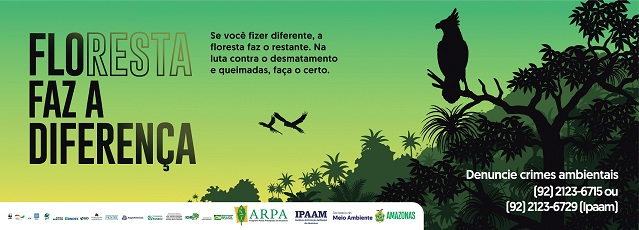
\includegraphics[width=5.90551in,height=2.125in]{./imgSAEB_7_POR/media/image16.png}

Disponível em :
\textless{}\href{https://meioambiente.am.gov.br/campanha-floresta-faz-a-diferenca/}{\uline{https://meioambiente.am.gov.br/campanha-floresta-faz-a-diferenca/}}\textgreater{}

Acesso em 6 de Abril 2023

Acima, pode-se ver um cartaz de conscientização sobre o desmatamento da
Amazônia. O uso e repetição de determinadas palavras e imagens tem como
finalidade sensibilizar os leitores para o problema do desmatamento.
Sobre o jogo de palavras presente no cartaz assinale a alternativa
correta:

\begin{enumerate}

\item
  As diferenças entre os tamanhos de fontes são os únicos elementos
  responsáveis pela persuasão.
\item
  O texto traz explicações sobre as consequências das queimadas e
  desmatamento
\item
  O uso das variações da palavra `diferença' e `diferente' que se
  articulam para convidar a uma mudança de atitude
\item
  As imagens são os recursos de maior função persuasiva
\end{enumerate}

SAEB: - Identificar o uso de recursos persuasivos em textos verbais e
não verbais.

Bncc: EF67LP07)Identificar o uso de recursos persuasivos em textos
argumentativos diversos (como a elaboração do título, escolhas lexicais,
construções metafóricas, a explicitação ou a ocultação de fontes de
informação) e perceber seus efeitos de sentido.

\begin{enumerate}
\def\labelenumi{\arabic{enumi}.}
\item
  Incorreta. A escolha de fontes, tamanhos e cores é um fator importante
  para a compreensão imediata da mensagem do texto, porém, não é o único
  recurso utilizado com essa finalidade.
\item
  Incorreta. Embora o texto faça alusão ao desmatamento e às queimadas,
  não se encontram explicações sobre os termos e suas consequências.
\item
  Correta. Os diversos recursos modais e o jogo de sentido no emprego
  das palavras destacadas são os principais recursos de persuasão,
  sensibilização e chamada para mudança de atitudes presente no cartaz.
\item
  Incorreta. Embora as imagens contribuam para a compreensão da
  mensagem, de forma isolada não contribuem para o sentido da mensagem.
\end{enumerate}

\num{2}

\textbf{Fumaça de queimadas do Amazonas chega a São Paulo; moradores
relatam ``cheiro forte''}

Segundo a Climatempo, a nuvem de fumaça foi gerada por incêndios em
parte do Amazonas, Acre e Mato Grosso

Moradores da cidade de São Paulo relataram sentir cheiro de fumaça na
manhã desta sexta-feira (9).

Na quinta (8), a Climatempo havia alertado para a nuvem gerada por
queimadas em parte do Amazonas, Acre e Mato Grosso, que espalhou sobre o
Brasil, e que chegaria também em grande parte do Centro-Oeste, no Paraná
e até em parte do estado de São Paulo.

A Companhia Ambiental do Estado de São Paulo (CETESB) disse que a
Divisão de Qualidade do Ar da agência está investigando as fumaças e
monitorando a qualidade do ar.

``{[}A divisão{]} está fazendo uma apuração detalhada dos dados das
estações de monitoramento da qualidade do ar distribuídas pela RMSP
Informaremos assim que tivermos um dado mais consolidado sobre a
ocorrência'', diz a nota.

Disponível em
\textless{}\href{https://www.cnnbrasil.com.br/nacional/fumaca-de-queimadas-do-amazonas-chega-a-sao-paulo-moradores-relatam-cheiro-forte/}{\uline{https://www.cnnbrasil.com.br/nacional/fumaca-de-queimadas-do-amazonas-chega-a-sao-paulo-moradores-relatam-cheiro-forte/}}\textgreater.
Acesso em 7 de abril de 2023.

Assinale a alternativa que contém a parte da notícia denominada linha
fina:

\begin{enumerate}

\item
  Fumaça de queimadas do Amazonas chega a São Paulo; moradores relatam
  ``cheiro forte''
\item
  ``{[}A divisão{]} está fazendo uma apuração detalhada dos dados das
  estações de monitoramento da qualidade do ar distribuídas pela RMSP
  Informaremos assim que tivermos um dado mais consolidado sobre a
  ocorrência'', diz a nota.
\item
  Moradores da cidade de São Paulo relataram sentir cheiro de fumaça na
  manhã desta sexta-feira (9).
\item
  Segundo a Climatempo, a nuvem de fumaça foi gerada por incêndios em
  parte do Amazonas, Acre e Mato Grosso
\end{enumerate}

Saeb: Identificar elementos constitutivos de textos pertencentes ao
domínio

jornalístico/midiático

\begin{enumerate}
\def\labelenumi{\arabic{enumi}.}
\item
  Incorreta. O trecho corresponde ao título da notícia.
\item
  Incorreta. O trecho corresponde ao corpo da notícia.
\item
  Incorreta. O trecho compõe o lide da notícia.
\item
  Correta. A linha fina aparece como uma introdução ao assunto da
  notícia e se localiza entre o título e lide.
\end{enumerate}

\num{3}

Uma parceria entre a Universidade Federal do Rio de Janeiro e a
Universidade Federal do Estado do Rio de Janeiro (Unirio) vem estudando
o vírus-T linfotrópico humano do tipo 1, o HTLV-1, retrovírus da mesma
família do HIV, associado a casos de leucemia e doenças
neurodegenerativas. A pesquisa recebeu investimento da Organização
Pan-Americana de Saúde (Opas/OMS) junto com outros estudos
latino-americanos e caribenhos que investigam doenças negligenciadas.
Embora descrito, na década de 1980, como um vírus associado ao câncer, o
HTLV ainda é pouco estudado e bastante desconhecido do público em geral.

\href{https://conexao.ufrj.br/2023/04/pesquisa-investiga-virus-negligenciado-que-pode-levar-a-doencas-neurodegenerativas-e-leucemia/}{\uline{https://conexao.ufrj.br/2023/04/pesquisa-investiga-virus-negligenciado-que-pode-levar-a-doencas-neurodegenerativas-e-leucemia/}}.
Acesso em 20 de Abr de 2023

O texto acima é um texto do gênero de divulgação científica pois:

\begin{enumerate}

\item
  traz informações técnicas e de difícil compreensão
\item
  é escrito de maneira formal e dirigido a cientistas e estudiosos
\item
  traz informações sobre fatos do cotidiano
\item
  traz informações científicas em linguagem clara e acessível ao público
  geral
\end{enumerate}

Identificar elementos constitutivos de gêneros de divulgação científica

\begin{enumerate}
\def\labelenumi{\arabic{enumi}.}
\item
  Incorreta. O texto não apresenta linguagem técnica
\item
  Incorreta. O texto não é destinado apenas a cientistas
\item
  Incorreta. O trecho não aborda fatos cotidianos
\item
  Correta. O texto faz uso de linguagem clara e acessível para divulgar
  estudos científicos para o público em geral
\end{enumerate}

\num{4}

Il.mº. Sra. Diretora da Escola Estadual Ulysses Guimarães

Mariana Amaral Santos, aluna regularmente matriculada no sétimo ano do
ensino fundamental desta escola, vem respeitosamente solicitar à V. Sa a
expedição dos documentos necessários à sua transferência para outro
estabelecimento de ensino.

Nestes termos, pede deferimento.

Curitiba, 24 de setembro de 2022.

Texto adaptado.

Os gêneros textuais reivindicatórios são textos que circulam no campo da
vida pública e possuem função social e estrutura específicas. O texto
acima é um modelo de Requerimento pois tem como objetivo:

\begin{enumerate}
\def\labelenumi{\arabic{enumi}.}
\item
  convencer o destinatário a realizar uma ação importante.
\item
  solicitar formalmente ao destinatário a realização de uma ação.
\item
  mudar o comportamento do destinatário a partir da realização de ações.
\item
  informar formalmente o destinatário acerca da solicitação de ações.
\end{enumerate}

Identificar formas de organização de textos normativos, legais e/ou
reivindicatórios.

Bncc (EF67LP17)Analisar, a partir do contexto de produção, a forma de
organização das cartas de solicitação e de reclamação (datação, forma de
início, apresentação contextualizada do pedido ou da reclamação, em
geral, acompanhada de explicações, argumentos e/ou relatos do problema,
fórmula de finalização mais ou menos cordata, dependendo do tipo de
carta e subscrição) e algumas das marcas linguísticas relacionadas à
argumentação, explicação ou relato de fatos, como forma de possibilitar
a escrita fundamentada de cartas como essas ou de postagens em canais
próprios de reclamações e solicitações em situações que envolvam
questões relativas à escola, à comunidade ou a algum dos seus membros.

\begin{enumerate}
\def\labelenumi{\arabic{enumi}.}
\item
  Incorreta. O texto não pretende convencer
\item
  Correta. O texto pretende solicitar uma transferência de instituição
\item
  Incorreta. Não há indicação de mudança de atitude
\item
  Incorreta. O objetivo não é informar e sim solicitar
\end{enumerate}

\num{5}

ATO I

Cena I

Veneza. Uma rua. Entram Antônio. Salarino e Salânio.

ANTÓNIO - Não sei, realmente, porque estou tão triste. Isso me enfara; e
a vós também, dissestes. Mas como começou essa tristeza, de que modo a
adquiri, como me veio, onde nasceu, de que matéria é feita, ainda estou
por saber. E de tal modo obtuso ela me deixa, que mui dificilmente me
conheço.

SALARINO - Vosso espírito voga em pleno oceano, onde vossos galeões de
altivas velas - como burgueses ricos e senhores das ondas, ou qual vista
aparatosa distendida no mar - olham por cima da multidão de humildes
traficantes que os saúdam, modestos, inclinando-se, quando perpassam com
tecidas asas.

Shakespeare, William. O Mercador de Venza. Disponível em
\href{http://www.dominiopublico.gov.br/download/texto/cv000094.pdf}{\uline{http://www.dominiopublico.gov.br/download/texto/cv000094.pdf}}.
Acesso em 20 de Abr. de 2023

O trecho acima apresenta certas características, como discurso direto,
indicações de falas de personagens e rubrica que são características do
gênero textual:

\begin{enumerate}

\item
  Dramático. Gênero dos textos criados para serem encenados
\item
  Poesia. Gênero composto por versos e estrofes
\item
  Conto. Gênero escrito em linguagem simples e com poucos personagens
\item
  Romance. Gênero que comporta narrativa longas e com muitos personagens
\end{enumerate}

Analisar elementos constitutivos de textos pertencentes ao domínio

literário.

\begin{enumerate}
\def\labelenumi{\arabic{enumi}.}
\item
  Correta. O texto acima é um exemplo de texto teatral ou dramático
\item
  Incorreta. O trecho acima não é composto por versos e estrofes
\item
  Incorreta. O trecho acima não apresenta características de conto
\item
  O trecho acima não possui características de conto
\end{enumerate}

\num{6}

Rogério Ceni deixou o São Paulo. Este é só mais um capítulo na história
de um clube que caminha a passos largos rumo ao buraco. A verdade é uma
só e dói para o apaixonado torcedor admitir: aquele São Paulo que era
modelo de administração e que num intervalo de três anos ganhou
Paulista, Libertadores, Mundial de Clubes e o tricampeonato brasileiro
acabou. Virou apenas lembrança.

\href{https://ge.globo.com/futebol/times/sao-paulo/noticia/2023/04/20/opiniao-vaidade-e-soberba-de-dirigentes-afundam-o-sao-paulo-rumo-a-um-futuro-preocupante.ghtml}{\uline{https://ge.globo.com/futebol/times/sao-paulo/noticia/2023/04/20/opiniao-vaidade-e-soberba-de-dirigentes-afundam-o-sao-paulo-rumo-a-um-futuro-preocupante.ghtml}}.
Acesso em 20 de Abr de 2023

A Notícia acima apresenta muitas opiniões e poucos fatos. Há um fato
expresso no texto por:

\begin{enumerate}

\item
  Este é só mais um capítulo na história de um clube
\item
  A verdade é uma só e dói para o apaixonado torcedor
\item
  um clube que caminha a passos largos rumo ao buraco
\item
  O São Paulo num intervalo de três anos ganhou Paulista, Libertadores
  (...)
\end{enumerate}

Saeb: Distinguir fatos de opiniões em textos

\begin{enumerate}
\def\labelenumi{\arabic{enumi}.}
\item
  Incorreta. Este trecho representa a opinião do jornalista
\item
  Incorreta. Este trecho representa a opinião do jornalista
\item
  Incorreta. Este trecho representa a opinião do jornalista
\item
  Correta. Este trecho apresenta um fato
\end{enumerate}

\num{7}


\includegraphics[width=4.16667in,height=1.57292in]{./imgSAEB_7_POR/media/image17.png}

\href{http://www.arionaurocartuns.com.br/search?q=moradia}{\uline{http://www.arionaurocartuns.com.br/search?q=moradia}}.
Acesso em 20 de Abr de 2023.

A charge utiliza de recursos verbais e não verbais para provocar:

\begin{enumerate}

\item
  Humor e reflexão
\item
  Crítica e tristeza
\item
  Humor e revolta
\item
  Crítica e alegria
\end{enumerate}

Saeb: Inferir, em textos multissemióticos, efeitos de humor, ironia e/ou
crítica.

Bncc: EF69LP03 Inferir e justificar, em textos multissemióticos --
tirinhas, charges, memes, gifs etc. --, o efeito de humor, ironia e/ou
crítica pelo uso ambíguo de palavras, expressões ou imagens ambíguas, de
clichês, de recursos iconográficos, de pontuação etc.

a)Correta. As charges em geral pretendem provocar humor e reflexão por
meio da crítica social

\begin{enumerate}
\def\labelenumi{\arabic{enumi}.}
\item
  Incorreta. Não pretende provocar tristeza, apesar de trazer temas
  difíceis
\item
  Incorreta. A charge não pretende causar revolta, embora provoque
  reflexão e crítica
\item
  Incorreta. A charge não pretende trazer mensagem de alegria
\end{enumerate}

\num{8}

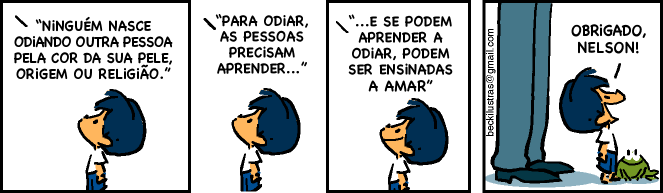
\includegraphics[width=5.90551in,height=1.72222in]{./imgSAEB_7_POR/media/image18.png}

\href{https://tirasarmandinho.tumblr.com/search/amor}{\uline{https://tirasarmandinho.tumblr.com/search/amor}}.
Acesso em 21 de Abr.

A tirinha acima faz referência a uma frase de Nelson Mandela. Sempre que
um texto faz referência a outro ou o toma como modelo de partida
utiliza-se o recurso chamado:

\begin{enumerate}

\item
  Persuasão
\item
  Coesão
\item
  Metáfora
\item
  Intertextualidade
\end{enumerate}

Saeb: Analisar a intertextualidade entre textos literários ou entre
estes e outros

textos verbais ou não verbais.

Bncc: (EF67LP27) Analisar, entre os textos literários e entre estes e
outras manifestações artísticas (como cinema, teatro, música, artes
visuais e midiáticas), referências explícitas ou implícitas a outros
textos, quanto aos temas, personagens e recursos literários e semióticos

\begin{enumerate}
\def\labelenumi{\arabic{enumi}.}
\item
  Incorreta. Este não é um recurso de persuasão
\item
  Incorreta. Este não é um recurso de coesão
\item
  Incorreta. Neste exemplo não ocorre o uso de metáfora
\item
  Correta. O uso de outros textos como modelo ou ponto de partida é
  chamado de intertextualidade.
\end{enumerate}

\num{9}

Leia o trecho a seguir:

``O Rio Doce, que nós, Krenak, chamamos de Watu, nosso avô,é uma pessoa,
não um recurso, como dizem os economistas''

Krenak, Ailton. Ideias para adiar o fim do mundo.2ª Ed. São paulo:
Companhia da Letras, 2020, p.~40

O trecho acima traz importantes informações sobre:

\begin{enumerate}

\item
  mitos e lendas que servem para ilustrar a cultura indígena
\item
  as diferenças entre a maneira de pensar os recursos naturais entre os
  indígenas e não indígenas
\item
  A língua falada pelos povos indígenas brasileiros no estado de Minas
  Gerais
\item
  uma história que é passada de geração em geração restrita aos povos
  indígenas brasileiros
\end{enumerate}

Saeb: Inferir a presença de valores sociais, culturais e humanos em
textos

literários.

Bncc:(EF69LP44) Inferir a presença de valores sociais, culturais e
humanos e de diferentes visões de mundo, em textos literários,
reconhecendo nesses textos formas de estabelecer múltiplos olhares sobre
as identidades, sociedades e culturas e considerando a autoria e o
contexto social e histórico de sua produção.

\begin{enumerate}
\def\labelenumi{\arabic{enumi}.}
\item
  Incorreta. O trecho não retrata um mito ou lenda
\item
  Correta. No trecho Ailton Krenak explica a maneira como os povos
  indígenas enxergam os recursos naturais
\item
  Incorreta. Apesar de trazer o termo utilizado para designar o rio, não
  traz informações sobre a língua
\item
  Incorreta. O trecho não faz referência à forma como essas questões são
  tratadas dentro da tradição indígena.
\end{enumerate}

\num{10}

Faxina correta da casa evita crise alérgica e possíveis problemas
respiratórios

Pessoas alérgicas devem evitar acúmulo de objetos dentro de casa,
principalmente no quarto.

Alérgica desde criança, a aposentada Glória Pordeus, 53 anos, viu os
problemas respiratórios serem agravados após se tornar portadora de
Lúpus, devido à baixa imunidade relacionada à doença. \textbf{Com isso,}
ela precisou redobrar os cuidados na hora de organizar a casa.
Especialistas alertam que pessoas alérgicas devem evitar acúmulo de
certos objetos, principalmente no quarto, e invés de usar vassoura para
limpar o chão, deve-se usar um pano úmido, e repassam dicas de como
manter o domicílio limpo sem comprometer a saúde.

\href{https://jornaldaparaiba.com.br/bichos/faxina-correta-da-casa-evita-crise-alergica-e-possiveis-problemas-respiratorios/}{\uline{https://jornaldaparaiba.com.br/bichos/faxina-correta-da-casa-evita-crise-alergica-e-possiveis-problemas-respiratorios/}}\textbf{.}

No texto acima, a expressão destacada se refere a:

\begin{enumerate}

\item
  Limpeza redobrada do ambiente
\item
  Condição de saúde que faz com que os cuidados tenham que ser
  redobrados
\item
  Orientação médica sobre os cuidados com as crianças
\item
  Idade da paciente que precisa se cuidar cada vez mais
\end{enumerate}

Analisar os mecanismos que contribuem para a progressão textual.

\begin{enumerate}
\def\labelenumi{\arabic{enumi}.}
\item
  Incorreta.Esta informação aparece depois do recurso
\item
  Correta. O termo refere-se às doenças que exigem mais cuidados na hora
  da limpeza
\end{enumerate}

c)Incorreta. O termo não se refere a orientações médicas, e sim ao que
leva a precisar de certos cuidados

\begin{enumerate}
\def\labelenumi{\arabic{enumi}.}
\tightlist
\item
  Incorreta. Apesar de trazer a informação sobre a idade o termo não se
  refere a isso e sim à condição de saúde
\end{enumerate}

\num{11}

Veja o título da notícia em negrito e responda

\hypertarget{sedentuxe1rios-e-grudados-a-uma-tela.-o-que-mostra-o-maior-estudo-mundial-sobre-atividade-fuxedsica-de-jovens}{%
\section{\texorpdfstring{\textbf{Sedentários e grudados a uma tela. O
que mostra o maior estudo mundial sobre atividade física de
jovens}}{Sedentários e grudados a uma tela. O que mostra o maior estudo mundial sobre atividade física de jovens}}\label{sedentuxe1rios-e-grudados-a-uma-tela.-o-que-mostra-o-maior-estudo-mundial-sobre-atividade-fuxedsica-de-jovens}}

\hypertarget{segundo-os-dados-divulgados-nesta-sexta-feira-80-dos-adolescentes-do-mundo-nuxe3o-fazem-o-muxednimo-de-exercuxedcio-recomendado.-para-as-meninas-os-nuxfameros-suxe3o-ainda-piores}{%
\section{Segundo os dados divulgados nesta sexta-feira, 80\% dos
adolescentes do mundo não fazem o mínimo de exercício recomendado. Para
as meninas, os números são ainda
piores}\label{segundo-os-dados-divulgados-nesta-sexta-feira-80-dos-adolescentes-do-mundo-nuxe3o-fazem-o-muxednimo-de-exercuxedcio-recomendado.-para-as-meninas-os-nuxfameros-suxe3o-ainda-piores}}

\href{https://brasil.elpais.com/brasil/2019/11/18/actualidad/1574086350_697117.html}{\uline{https://brasil.elpais.com/brasil/2019/11/18/actualidad/1574086350\_697117.html}}.
Acesso em 20 de Abr de 2023

A frase que apresenta uma hipérbole é:

\begin{enumerate}

\item
  Sedentários e grudados a uma tela
\item
  O queria o maior estudo mundial
\item
  adolescentes do mundo não fazem o mínimo
\item
  Para as meninas os números são ainda piores
\end{enumerate}

Saeb:Analisar o uso de figuras de linguagem como estratégia
argumentativa

\begin{enumerate}
\def\labelenumi{\arabic{enumi}.}
\item
  Correta. O termo grudados a uma tela representa figura de linguagem
\item
  Incorreta. O termo não apresenta figura de linguagem
\item
  Incorreta. O termo não apresenta figura de linguagem
\item
  Incorreta. O termo não apresenta figura de linguagem
\end{enumerate}

\num{12}

Os especialistas consultados consideram que o mais previsível durante as
próximas semanas é ``um crescimento substancial das detecções da
ômicron, que já começa a ser percebido, até que a nova variante
substitua a delta, \textbf{algo que poderia ocorrer} em cerca de três
semanas'', explica Federico García, chefe de Microbiologia do Hospital
San Cecilio (Granada), um centro de referência para a Andaluzia
oriental.

\href{https://brasil.elpais.com/internacional/2021-12-13/agencia-de-saude-publica-da-ue-avisa-que-a-omicron-se-propaga-pelo-continente-mais-rapido-do-que-e-detectada.html}{\uline{https://brasil.elpais.com/internacional/2021-12-13/agencia-de-saude-publica-da-ue-avisa-que-a-omicron-se-propaga-pelo-continente-mais-rapido-do-que-e-detectada.html}}.
Acesso em 21 de Abr de 2023

A expressão em destaque é um conectivo de coesão textual. A palavra algo
no texto se refere a:

\begin{enumerate}

\item
  acontecimentos inesperados
\item
  crescimento das detecções
\item
  substituição da variante ômicron pela delta
\item
  mortes por covid
\end{enumerate}

Saeb:Analisar os processos de referenciação lexical e pronominal.

\begin{enumerate}
\def\labelenumi{\arabic{enumi}.}
\item
  Incorreta. O conectivo não se refere a acontecimentos inesperados
\item
  Incorreta. Embora esteja na mesma frase, algo não se refere a este
  fato
\item
  Correta. O cientista afirma que a substituição deve ocorrer em cerca
  de três semanas
\item
  Incorreta. O texto não traz informações sobre mortes por covid
\end{enumerate}

\num{13}

\textbf{A prática da leitura é o grande desafio da escola e das famílias
para os alunos e filhos. É comum encontrarmos aqueles que não gostam de
ler --} mas isso só até descobrirem o prazer dessa atividade. Se as
crianças fossem estimuladas no lado prazeroso da leitura, teríamos mais
leitores e não apenas compradores de livros. \textbf{A literatura é um
dos principais meios de transmissão cultural e,} como nos mantém em
contato com a imaginação, estimula a nossa criatividade.

https://g1.globo.com/Noticias/Vestibular/0,,MUL723077-5604,00-OPINIAO+COMO+FAZER+DE+SEU+FILHO+UM+LEITOR.html

Os trechos em destaque apresentam argumentação do tipo

\begin{enumerate}

\item
  Argumento de autoridade
\item
  Argumento de exemplo
\item
  Argumento de consenso
\item
  Argumento por ilustração
\end{enumerate}

Avaliar a eficácia das estratégias argumentativas em textos de
diferentes gêneros.

\begin{enumerate}
\def\labelenumi{\arabic{enumi}.}
\item
  Incorreta. O trecho não cita quem profere as afirmações, portanto não
  se sabe se é um argumento de autoridade
\item
  Incorreta. O trecho não traz exemplos
\item
  Correta. O trecho utiliza de argumentos que, em geral, não geram
  discordância
\item
  Incorreta. Neste caso, não são citados exemplos como estratégia de
  argumentação
\end{enumerate}

\num{14}

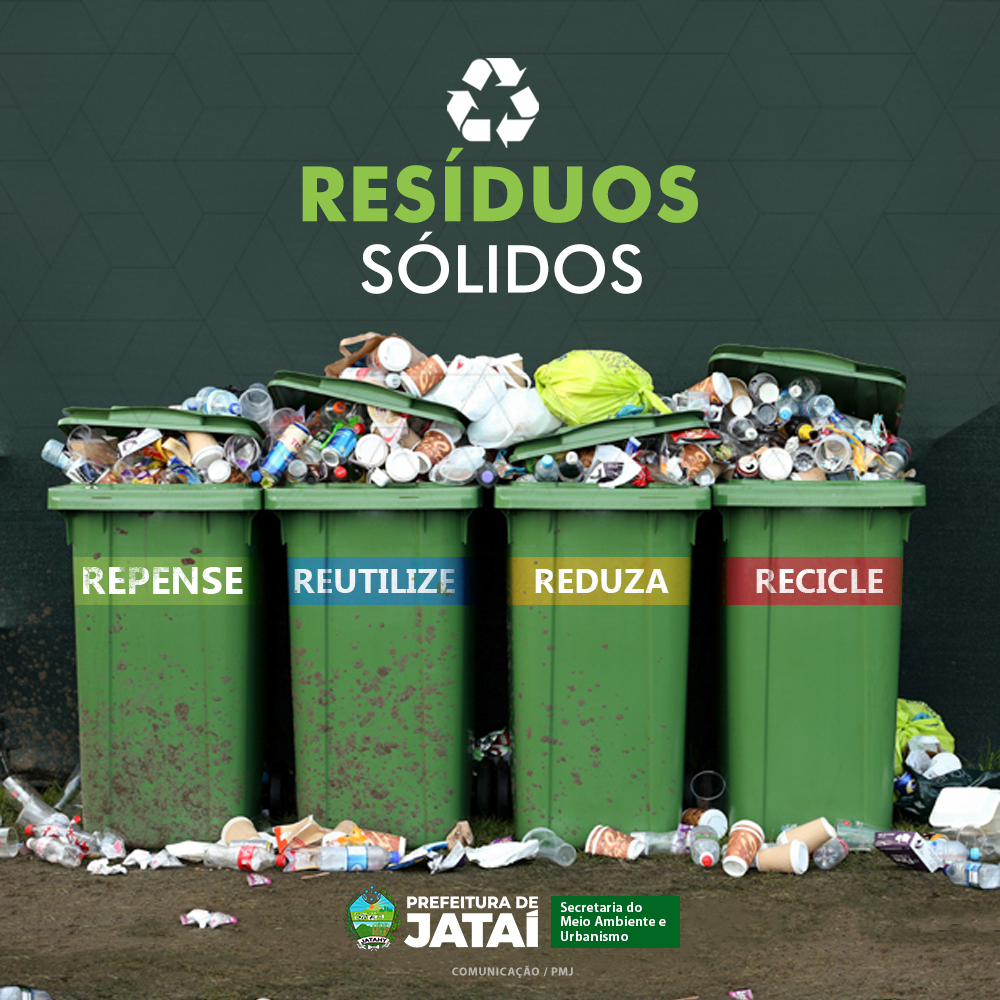
\includegraphics[width=5.90551in,height=5.90278in]{./imgSAEB_7_POR/media/image19.png}

\href{https://www.jatai.go.gov.br/separe-seu-lixo-de-forma-adequada/}{\uline{https://www.jatai.go.gov.br/separe-seu-lixo-de-forma-adequada/}}.Acesso
em 22 de Abr de 2023

Na imagem acima, pode-se perceber diversos recursos para que a mensagem
seja transmitida de maneira eficiente e imediata. No caso da escolha dos
verbos utilizados é correto afirmar que:

\begin{enumerate}

\item
  Os verbos no imperativo afirmativo sugerem uma ação
\item
  O uso dos verbos no infinitivo indica uma instrução
\item
  Os verbos no subjuntivo indicam uma advertência
\item
  O uso dos verbos no infinitivo indica uma ordem
\end{enumerate}

Analisar os efeitos de sentido dos tempos, modos e/ou vozes verbais com
base no gênero textual e na intenção comunicativa.

\begin{enumerate}
\def\labelenumi{\arabic{enumi}.}
\item
  Correta. O verbo no modo imperativo tem a função de instrução e neste
  caso, de maneira afirmativa, sugere uma mudança de atitude por parte
  do leitor
\item
  Incorreta.Os verbos não estão no infinitivo
\item
  Incorreta. Os verbos não estão no modo subjuntivo e não indicam
  advertência
\item
  Incorreta. O uso de verbos no imperativo, como no exemplo podem
  indicar uma ordem, porém a imagem não traz verbos no infinitivo
\end{enumerate}

\num{15}


\includegraphics[width=5.90551in,height=3.15278in]{./imgSAEB_7_POR/media/image20.png}

\href{https://www.tre-sp.jus.br/comunicacao/noticias/2022/Marco/tuitaco-roledaseleicoes-alcanca-trending-topics-no-twitter}{\uline{https://www.tre-sp.jus.br/comunicacao/noticias/2022/Marco/tuitaco-roledaseleicoes-alcanca-trending-topics-no-twitter}}.
Acesso em 20 de Abr de 2023

Analisando a campanha acima, destinada ao público jovem, é correto
afirmar que:

\begin{enumerate}

\item
  a campanha utiliza linguagem formal para atingir o público alvo
\item
  a campanha utiliza linguagem informal para atingir todos os públicos
\item
  a campanha utiliza linguagem informal para atingir o público alvo
\item
  a campanha utiliza linguagem formal para atingir todos os públicos
\end{enumerate}

Avaliar a adequação das variedades linguísticas em contextos de uso.

\begin{enumerate}
\def\labelenumi{\arabic{enumi}.}
\item
  Incorreta. A campanha não utiliza linguagem formal
\item
  Incorreta. Apesar de fazer uso da linguagem informal a campanha tem um
  público alvo bem claro
\item
  Correta. A campanha faz uso de linguagem informal para atingir os
  jovens
\item
  Incorreta. A campanha não faz uso de linguagem formal, nem pretende
  atingir todos os públicos
\end{enumerate}
